% Options for packages loaded elsewhere
% Options for packages loaded elsewhere
\PassOptionsToPackage{unicode}{hyperref}
\PassOptionsToPackage{hyphens}{url}
%
\documentclass[
  10pt,
  ignorenonframetext,
  aspectratio=169,
  t]{beamer}
\newif\ifbibliography
\usepackage{pgfpages}
\setbeamertemplate{caption}[numbered]
\setbeamertemplate{caption label separator}{: }
\setbeamercolor{caption name}{fg=normal text.fg}
\beamertemplatenavigationsymbolsempty
% remove section numbering
\setbeamertemplate{part page}{
  \centering
  \begin{beamercolorbox}[sep=16pt,center]{part title}
    \usebeamerfont{part title}\insertpart\par
  \end{beamercolorbox}
}
\setbeamertemplate{section page}{
  \centering
  \begin{beamercolorbox}[sep=12pt,center]{section title}
    \usebeamerfont{section title}\insertsection\par
  \end{beamercolorbox}
}
\setbeamertemplate{subsection page}{
  \centering
  \begin{beamercolorbox}[sep=8pt,center]{subsection title}
    \usebeamerfont{subsection title}\insertsubsection\par
  \end{beamercolorbox}
}
% Prevent slide breaks in the middle of a paragraph
\widowpenalties 1 10000
\raggedbottom
\AtBeginPart{
  \frame{\partpage}
}
\AtBeginSection{
  \ifbibliography
  \else
    \frame{\sectionpage}
  \fi
}
\AtBeginSubsection{
  \frame{\subsectionpage}
}
\usepackage{iftex}
\ifPDFTeX
  \usepackage[T1]{fontenc}
  \usepackage[utf8]{inputenc}
  \usepackage{textcomp} % provide euro and other symbols
\else % if luatex or xetex
  \usepackage{unicode-math} % this also loads fontspec
  \defaultfontfeatures{Scale=MatchLowercase}
  \defaultfontfeatures[\rmfamily]{Ligatures=TeX,Scale=1}
\fi
\usepackage{lmodern}

\ifPDFTeX\else
  % xetex/luatex font selection
\fi
% Use upquote if available, for straight quotes in verbatim environments
\IfFileExists{upquote.sty}{\usepackage{upquote}}{}
\IfFileExists{microtype.sty}{% use microtype if available
  \usepackage[]{microtype}
  \UseMicrotypeSet[protrusion]{basicmath} % disable protrusion for tt fonts
}{}
\makeatletter
\@ifundefined{KOMAClassName}{% if non-KOMA class
  \IfFileExists{parskip.sty}{%
    \usepackage{parskip}
  }{% else
    \setlength{\parindent}{0pt}
    \setlength{\parskip}{6pt plus 2pt minus 1pt}}
}{% if KOMA class
  \KOMAoptions{parskip=half}}
\makeatother

\usepackage{color}
\usepackage{fancyvrb}
\newcommand{\VerbBar}{|}
\newcommand{\VERB}{\Verb[commandchars=\\\{\}]}
\DefineVerbatimEnvironment{Highlighting}{Verbatim}{commandchars=\\\{\}}
% Add ',fontsize=\small' for more characters per line
\usepackage{framed}
\definecolor{shadecolor}{RGB}{241,243,245}
\newenvironment{Shaded}{\begin{snugshade}}{\end{snugshade}}
\newcommand{\AlertTok}[1]{\textcolor[rgb]{0.68,0.00,0.00}{#1}}
\newcommand{\AnnotationTok}[1]{\textcolor[rgb]{0.37,0.37,0.37}{#1}}
\newcommand{\AttributeTok}[1]{\textcolor[rgb]{0.40,0.45,0.13}{#1}}
\newcommand{\BaseNTok}[1]{\textcolor[rgb]{0.68,0.00,0.00}{#1}}
\newcommand{\BuiltInTok}[1]{\textcolor[rgb]{0.00,0.23,0.31}{#1}}
\newcommand{\CharTok}[1]{\textcolor[rgb]{0.13,0.47,0.30}{#1}}
\newcommand{\CommentTok}[1]{\textcolor[rgb]{0.37,0.37,0.37}{#1}}
\newcommand{\CommentVarTok}[1]{\textcolor[rgb]{0.37,0.37,0.37}{\textit{#1}}}
\newcommand{\ConstantTok}[1]{\textcolor[rgb]{0.56,0.35,0.01}{#1}}
\newcommand{\ControlFlowTok}[1]{\textcolor[rgb]{0.00,0.23,0.31}{\textbf{#1}}}
\newcommand{\DataTypeTok}[1]{\textcolor[rgb]{0.68,0.00,0.00}{#1}}
\newcommand{\DecValTok}[1]{\textcolor[rgb]{0.68,0.00,0.00}{#1}}
\newcommand{\DocumentationTok}[1]{\textcolor[rgb]{0.37,0.37,0.37}{\textit{#1}}}
\newcommand{\ErrorTok}[1]{\textcolor[rgb]{0.68,0.00,0.00}{#1}}
\newcommand{\ExtensionTok}[1]{\textcolor[rgb]{0.00,0.23,0.31}{#1}}
\newcommand{\FloatTok}[1]{\textcolor[rgb]{0.68,0.00,0.00}{#1}}
\newcommand{\FunctionTok}[1]{\textcolor[rgb]{0.28,0.35,0.67}{#1}}
\newcommand{\ImportTok}[1]{\textcolor[rgb]{0.00,0.46,0.62}{#1}}
\newcommand{\InformationTok}[1]{\textcolor[rgb]{0.37,0.37,0.37}{#1}}
\newcommand{\KeywordTok}[1]{\textcolor[rgb]{0.00,0.23,0.31}{\textbf{#1}}}
\newcommand{\NormalTok}[1]{\textcolor[rgb]{0.00,0.23,0.31}{#1}}
\newcommand{\OperatorTok}[1]{\textcolor[rgb]{0.37,0.37,0.37}{#1}}
\newcommand{\OtherTok}[1]{\textcolor[rgb]{0.00,0.23,0.31}{#1}}
\newcommand{\PreprocessorTok}[1]{\textcolor[rgb]{0.68,0.00,0.00}{#1}}
\newcommand{\RegionMarkerTok}[1]{\textcolor[rgb]{0.00,0.23,0.31}{#1}}
\newcommand{\SpecialCharTok}[1]{\textcolor[rgb]{0.37,0.37,0.37}{#1}}
\newcommand{\SpecialStringTok}[1]{\textcolor[rgb]{0.13,0.47,0.30}{#1}}
\newcommand{\StringTok}[1]{\textcolor[rgb]{0.13,0.47,0.30}{#1}}
\newcommand{\VariableTok}[1]{\textcolor[rgb]{0.07,0.07,0.07}{#1}}
\newcommand{\VerbatimStringTok}[1]{\textcolor[rgb]{0.13,0.47,0.30}{#1}}
\newcommand{\WarningTok}[1]{\textcolor[rgb]{0.37,0.37,0.37}{\textit{#1}}}

\usepackage{longtable,booktabs,array}
\newcounter{none} % for unnumbered tables
\usepackage{calc} % for calculating minipage widths
\usepackage{caption}
% Make caption package work with longtable
\makeatletter
\def\fnum@table{\tablename~\thetable}
\makeatother
\usepackage{graphicx}
\makeatletter
\newsavebox\pandoc@box
\newcommand*\pandocbounded[1]{% scales image to fit in text height/width
  \sbox\pandoc@box{#1}%
  \Gscale@div\@tempa{\textheight}{\dimexpr\ht\pandoc@box+\dp\pandoc@box\relax}%
  \Gscale@div\@tempb{\linewidth}{\wd\pandoc@box}%
  \ifdim\@tempb\p@<\@tempa\p@\let\@tempa\@tempb\fi% select the smaller of both
  \ifdim\@tempa\p@<\p@\scalebox{\@tempa}{\usebox\pandoc@box}%
  \else\usebox{\pandoc@box}%
  \fi%
}
% Set default figure placement to htbp
\def\fps@figure{htbp}
\makeatother





\setlength{\emergencystretch}{3em} % prevent overfull lines

\providecommand{\tightlist}{%
  \setlength{\itemsep}{0pt}\setlength{\parskip}{0pt}}



 


\setbeamertemplate{frametitle continuation}{}
\setbeamertemplate{itemize items}[circle]
\usepackage{caption}
\usepackage{textpos}
\setlength{\TPHorizModule}{1cm}
\setlength{\TPVertModule}{1cm}

% credit line
\newcommand{\credit}{\scriptsize\textcolor{gray!70!black}{\quad courtiol@izw-berlin.de | \url{www.datazoogang.de} | \url{www.izw-berlin.de/en}}}

% create footer with slide number
\setbeamertemplate{footline}{%
  \credit\hfill\usebeamercolor[fg]{page number in head/foot}%
  \usebeamerfont{page number in head/foot}%
  \insertframenumber{} / \inserttotalframenumber\kern1em\vskip2pt%
}

\usepackage{colortbl}
\usepackage{makecell}
\usepackage{tcolorbox}
\tcbuselibrary{skins}
\usepackage{etoolbox}
\usepackage{forest}
\usepackage{amssymb}

% make the red boxes around important stuff
\newtcolorbox{callout}{%
  colback=white,
  colframe=red,
  boxrule=1pt,
  arc=6pt,
  boxsep=2pt,
  left=8pt,
  right=8pt,
  top=4pt,
  bottom=4pt,
  before skip=6pt, % space before the box
  after skip=6pt   % space after the box
}

% 95% CI
\newcommand{\ci}{\ensuremath{\text{CI}_{\text{95\%}}}}

% highlights
\newcommand{\bluenorm}[1]{\textcolor{bluebeamer}{#1}}
\newcommand{\blueit}[1]{\textcolor{bluebeamer}{\emph{#1}}}
\newcommand{\bluebold}[1]{\textcolor{bluebeamer}{\textbf{#1}}}

% define some custom colours
\definecolor{okgreen}{HTML}{00CC99}
\definecolor{bad}{HTML}{FF5050}
\definecolor{bluebeamer}{HTML}{3333B3}
\usepackage{xcolor} % for other colours

\captionsetup{labelformat=empty, justification=centering}

% for displaying section slides (with center alignment)
\AtBeginSection[]{
  \begin{frame}[c]
  \centering
  \Large\insertsectionhead
  \end{frame}
}

% for grey background behind in-line R code
\let\oldtexttt\texttt
\renewcommand{\texttt}[1]{\colorbox{gray!20}{\oldtexttt{#1}}}
\makeatletter
\@ifpackageloaded{caption}{}{\usepackage{caption}}
\AtBeginDocument{%
\ifdefined\contentsname
  \renewcommand*\contentsname{Table of contents}
\else
  \newcommand\contentsname{Table of contents}
\fi
\ifdefined\listfigurename
  \renewcommand*\listfigurename{List of Figures}
\else
  \newcommand\listfigurename{List of Figures}
\fi
\ifdefined\listtablename
  \renewcommand*\listtablename{List of Tables}
\else
  \newcommand\listtablename{List of Tables}
\fi
\ifdefined\figurename
  \renewcommand*\figurename{Figure}
\else
  \newcommand\figurename{Figure}
\fi
\ifdefined\tablename
  \renewcommand*\tablename{Table}
\else
  \newcommand\tablename{Table}
\fi
}
\@ifpackageloaded{float}{}{\usepackage{float}}
\floatstyle{ruled}
\@ifundefined{c@chapter}{\newfloat{codelisting}{h}{lop}}{\newfloat{codelisting}{h}{lop}[chapter]}
\floatname{codelisting}{Listing}
\newcommand*\listoflistings{\listof{codelisting}{List of Listings}}
\makeatother
\makeatletter
\makeatother
\makeatletter
\@ifpackageloaded{caption}{}{\usepackage{caption}}
\@ifpackageloaded{subcaption}{}{\usepackage{subcaption}}
\makeatother

\usepackage{bookmark}
\IfFileExists{xurl.sty}{\usepackage{xurl}}{} % add URL line breaks if available
\urlstyle{same}
% fallback for those not using the hyperref driver hyperxmp:
\makeatletter
\@ifundefined{xmpquote}{\newcommand{\xmpquote}[1]{#1}}{}
\makeatother
\hypersetup{
  pdftitle={Introduction to Basic and Advanced Statistical Modelling},
  pdfauthor={Alexandre Courtiol},
  hidelinks,
  pdfcreator={LaTeX via pandoc}}


\title{\texorpdfstring{Introduction to Basic and Advanced Statistical
Modelling}{Introduction to Basic and Advanced Statistical Modelling}}
\subtitle{\texorpdfstring{From LM to GLM}{From LM to GLM}}
\author{Alexandre Courtiol}
\date{}

\begin{document}
\frame{\titlepage}

\renewcommand*\contentsname{Table of contents}
\begin{frame}[allowframebreaks]
  \frametitle{Table of contents}
  \setcounter{tocdepth}{3}
  \tableofcontents
\end{frame}
\setcounter{tocdepth}{3}
\tableofcontents
}

\section{Linear Models (LM)}\label{linear-models-lm}

\begin{frame}{LM --- what is a statistical model?}
\protect\phantomsection\label{lm-what-is-a-statistical-model}
\bluebold{Statistical model}

an approximate description of the \blueit{data generating process},
i.e.~an approximation of how the world generates data

\pause

\vspace{1em}

\textbf{NB:} seeing models as a \blueit{data generating process} may not
be intuitive at first, but it is both conceptually and practically
crucial!

\vspace{1em}

In particular, it helps

\begin{itemize}
\tightlist
\item
  correctly interpreting model parameters
\item
  planning sample size before data collection
\item
  testing the coverage of confidence intervals (i.e.~do they work as
  intended)
\item
  testing the robustness of the statistical test (i.e.~check the rate of
  false positives)
\item
  performing prior and posterior predictive checks during Bayesian
  analyses
\end{itemize}
\end{frame}

\begin{frame}{LM --- what is a linear model (LM)?}
\protect\phantomsection\label{lm-what-is-a-linear-model-lm}
\bluebold{Linear model}

a data generating process produced by a \blueit{linear function}: the
data are generated from a set of terms by multiplying each term by a
constant (a model parameter) and summing them

\pause

\vspace{1em}

\textbf{NB:}

\begin{itemize}
\tightlist
\item
  linear models encompass the classic linear regression which forms a
  straight line, but also many other models (e.g.~polynomials are linear
  and yet do not form straight lines) \(\rightarrow\) LM are linear in
  parameters (not necessarily in variables)
\item
  much of the difficulty people encounter when dealing with more complex
  models (e.g.~Generalised Linear Models, Linear Mixed-effects Models,
  Hierarchical Models) is often caused by not having sufficiently
  understood the LM
\end{itemize}
\end{frame}

\begin{frame}{LM --- notations of a LM: simple notation}
\protect\phantomsection\label{lm-notations-of-a-lm-simple-notation}
\vspace{1em}

\begin{center}
$y_i = \beta_0 + \beta_1 \times x_{1,i} + \beta_2 \times x_{2,i} + \dots + \beta_{p} \times x_{p,i} + \epsilon_i$ with $\epsilon_i \sim \mathcal{N}(0, \sigma^2)$
\end{center}

\pause

\vspace{1em}

\begin{itemize}
\tightlist
\item
  \(y_i\) = the response variable / dependent variable / observations to
  explain
\item
  \(\beta_j\) = the model parameters / regression coefficients
\item
  \(x_{j,i}\) = regressors / constants derived from the predictor
  variables (aka predictors for short)
\item
  \(\epsilon_i\) = the errors / residual errors
\end{itemize}

\pause

\vspace{1em}

\textbf{NB:}

\begin{itemize}
\tightlist
\item
  this is the notation that biologists should use in their paper/thesis
  to describe their model
\item
  the regressors are sometimes directly given by the columns from your
  dataset (i.e.~the predictors), but not always (more on that later)
\item
  when parameters are not known but estimated they should wear a hat
  (e.g.~\(\hat{\beta_0}\)) and \(\epsilon_i\) (also sometimes called
  \(\varepsilon_i\)) usually becomes \(e_i\) or \(r_i\)
\end{itemize}
\end{frame}

\begin{frame}[fragile]{LM --- notations of a LM: usual R notation}
\protect\phantomsection\label{lm-notations-of-a-lm-usual-r-notation}
\vspace{1em}

\texttt{y\ \textasciitilde{}\ x\_1\ +\ x\_2\ +\ ...\ +\ x\_p}

\vspace{1em}

\textbf{NB:}

\begin{itemize}
\tightlist
\item
  the parameters and the error term are not written down
\end{itemize}
\end{frame}

\begin{frame}{LM --- notations of a LM: matrix notation}
\protect\phantomsection\label{lm-notations-of-a-lm-matrix-notation}
\vspace{1em}

\begin{center}
$Y = X \beta + \epsilon$
\end{center}

\[
\begin{bmatrix} y_1 \\ y_2 \\ y_3 \\ \dots \\ y_n \end{bmatrix} =
\begin{bmatrix}
1 & x_{1,1} & x_{1,2} & \dots & x_{1,p} \\
1 & x_{2,1} & x_{2,2} & \dots & x_{2,p} \\
1 & x_{3,1} & x_{3,2} & \dots & x_{3,p} \\
\dots & \dots & \dots & \dots & \dots \\
1 & x_{n,1} & x_{n,2} & \dots & x_{n,p}
\end{bmatrix}
\begin{bmatrix}
\beta_0 \\ \beta_1 \\ \beta_2 \\ \dots \\ \beta_p
\end{bmatrix} +
\begin{bmatrix}
\epsilon_1 \\ \epsilon_2 \\ \epsilon_3 \\ \dots \\ \epsilon_n
\end{bmatrix}
\]

\pause

\begin{itemize}
\tightlist
\item
  \(Y\) = the vector of observations
\item
  \(X\) = a matrix called the design (or model) matrix
\item
  \(\beta\) = the vector of model parameters
\item
  \(\epsilon\) = the vector of errors, with again
  \(\epsilon_i \sim \mathcal{N}(0, \sigma^2)\)
\end{itemize}

\vspace{1em}

\textbf{NB:} this is the notation for statisticians and computer
scientists, which is particularly useful when interpreting coefficients
\end{frame}

\begin{frame}[fragile]{LM --- data generating process: data simulation}
\protect\phantomsection\label{lm-data-generating-process-data-simulation}
Let's enter \bluebold{God mode} \(\rightarrow\) we pretend that
\bluenorm{Emerald Lion} (a goddess) knows how her world generates data;
she informed us that in her world aliens keep growing with the number of
humans they eat as follows:

\begin{equation*}
\begin{cases}
\text{size}_i = 50 + 1.5 \times \text{humans\_eaten}_{i} + \epsilon_i \\
\epsilon_i \sim \mathcal{N}(0, \sigma^2 = 4)
\end{cases}
\end{equation*}

\pause

We can thus generate the size of 12 aliens that have eaten 1--3 humans
following E.L.'s recipe:

\footnotesize

\begin{Shaded}
\begin{Highlighting}[]
\FunctionTok{set.seed}\NormalTok{(}\DecValTok{2}\NormalTok{)}
\NormalTok{N }\OtherTok{\textless{}{-}} \DecValTok{12}
\NormalTok{Alien }\OtherTok{\textless{}{-}} \FunctionTok{tibble}\NormalTok{(}\AttributeTok{humans\_eaten =} \FunctionTok{rep}\NormalTok{(}\DecValTok{1}\SpecialCharTok{:}\DecValTok{3}\NormalTok{, }\AttributeTok{each =} \DecValTok{4}\NormalTok{), }\CommentTok{\# alternative e.g. rpois() would do }
                \AttributeTok{intercept =} \DecValTok{50}\NormalTok{, }\AttributeTok{slope =} \FloatTok{1.5}\NormalTok{,}
                \AttributeTok{error =} \FunctionTok{rnorm}\NormalTok{(}\AttributeTok{n =}\NormalTok{ N, }\AttributeTok{mean =} \DecValTok{0}\NormalTok{, }\AttributeTok{sd =} \DecValTok{2}\NormalTok{), }\CommentTok{\# must be rnorm!}
                \AttributeTok{size =}\NormalTok{ intercept }\SpecialCharTok{+}\NormalTok{ slope}\SpecialCharTok{*}\NormalTok{humans\_eaten }\SpecialCharTok{+}\NormalTok{ error)}
\end{Highlighting}
\end{Shaded}

\normalsize

\pause

\textbf{NB:} we could also write the last 2 lines as:

\footnotesize

\begin{Shaded}
\begin{Highlighting}[]
\NormalTok{size }\OtherTok{\textless{}{-}} \FunctionTok{rnorm}\NormalTok{(}\AttributeTok{n =} \DecValTok{12}\NormalTok{, }\AttributeTok{mean =}\NormalTok{ intercept }\SpecialCharTok{+}\NormalTok{ slope}\SpecialCharTok{*}\NormalTok{humans\_eaten, }\AttributeTok{sd =} \DecValTok{2}\NormalTok{)}
\end{Highlighting}
\end{Shaded}

\normalsize
\end{frame}

\begin{frame}[fragile]{LM --- data generating process: data check}
\protect\phantomsection\label{lm-data-generating-process-data-check}
\bluebold{Simulated data}

\footnotesize

\begin{Shaded}
\begin{Highlighting}[]
\NormalTok{Alien}
\end{Highlighting}
\end{Shaded}

\begin{verbatim}
# A tibble: 12 x 5
  humans_eaten intercept slope  error  size
         <int>     <dbl> <dbl>  <dbl> <dbl>
1            1        50   1.5 -1.79   49.7
2            1        50   1.5  0.370  51.9
3            1        50   1.5  3.18   54.7
4            1        50   1.5 -2.26   49.2
5            2        50   1.5 -0.161  52.8
# i 7 more rows
\end{verbatim}

\normalsize

\begin{itemize}
\tightlist
\item
  which columns show the \blueit{model parameters}?
\item
  which columns show \blueit{regressor} (here = predictor)?
\item
  which columns show \blueit{errors}?
\item
  which columns show \blueit{response variable}?
\end{itemize}
\end{frame}

\begin{frame}[fragile]{Practice 1}
\protect\phantomsection\label{practice-1}
\bluebold{Simulated data}

\footnotesize

\begin{Shaded}
\begin{Highlighting}[]
\NormalTok{Alien}
\end{Highlighting}
\end{Shaded}

\begin{verbatim}
# A tibble: 12 x 5
  humans_eaten intercept slope  error  size
         <int>     <dbl> <dbl>  <dbl> <dbl>
1            1        50   1.5 -1.79   49.7
2            1        50   1.5  0.370  51.9
3            1        50   1.5  3.18   54.7
4            1        50   1.5 -2.26   49.2
5            2        50   1.5 -0.161  52.8
# i 7 more rows
\end{verbatim}

\normalsize

\begin{itemize}
\tightlist
\item
  which columns show the \blueit{model parameters}?
\item
  which columns show \blueit{regressor} (here = predictor)?
\item
  which columns show \blueit{errors}?
\item
  which columns show \blueit{response variable}?
\item
  \textcolor{red}{what would the \blueit{mean response value} be, for an alien who does not eat humans?}
\item
  \textcolor{red}{what would the \blueit{mean response value} be, for an alien who eats 2 humans?}
\end{itemize}
\end{frame}

\begin{frame}{Solution}
\protect\phantomsection\label{solution}
\vfill

\begin{itemize}
\tightlist
\item
  \textcolor{red}{what would the \blueit{mean response value} be, for an alien who does not eat humans?}
\end{itemize}

\begin{center}
$\text{mean}(y \mid \text{humans\_eaten}=0) = 50 + 1.5 \times 0 = 50$
\end{center}

\pause

\vspace{1cm}

\begin{itemize}
\tightlist
\item
  \textcolor{red}{what would the \blueit{mean response value} be, for an alien who eats 2 humans?}
\end{itemize}

\begin{center}
$\text{mean}(y \mid \text{humans\_eaten}=2) = 50 + 1.5 \times 2 = 53$
\end{center}

\vfill
\end{frame}

\begin{frame}[fragile]{LM --- model fitting: frequentist approach}
\protect\phantomsection\label{lm-model-fitting-frequentist-approach}
In practice, model parameters are \bluenorm{unknown}, so we have to
estimate them\\
\(\rightarrow\) that is the whole point of statistical modelling\ldots{}
\(\rightarrow\) the God mode is now off

\pause

\begin{itemize}
\tightlist
\item
  in frequentist statistics, \blueit{fitting the model} means estimating
  the values of the model parameters that maximise the probability of
  the data
\end{itemize}

\vspace{1em}

\footnotesize

\begin{Shaded}
\begin{Highlighting}[]
\NormalTok{fit\_alien\_lm }\OtherTok{\textless{}{-}} \FunctionTok{lm}\NormalTok{(size }\SpecialCharTok{\textasciitilde{}}\NormalTok{ humans\_eaten, }\AttributeTok{data =}\NormalTok{ Alien)}
\FunctionTok{summary}\NormalTok{(fit\_alien\_lm) }\CommentTok{\# or coef(fit\_alien\_lm) for a focus on coefficients only}
\end{Highlighting}
\end{Shaded}

\normalsize

\tiny

\begin{verbatim}

Call:
lm(formula = size ~ humans_eaten, data = Alien)

Residuals:
    Min      1Q  Median      3Q     Max 
-1.9710 -1.1744 -0.4725  0.7023  3.4655 

Coefficients:
             Estimate Std. Error t value Pr(>|t|)    
(Intercept)   48.8353     1.3454  36.298 5.99e-12 ***
humans_eaten   2.3749     0.6228   3.813  0.00341 ** 
---
Signif. codes:  0 '***' 0.001 '**' 0.01 '*' 0.05 '.' 0.1 ' ' 1

Residual standard error: 1.762 on 10 degrees of freedom
Multiple R-squared:  0.5925,    Adjusted R-squared:  0.5518 
F-statistic: 14.54 on 1 and 10 DF,  p-value: 0.003411
\end{verbatim}

\normalsize
\end{frame}

\begin{frame}[fragile]{LM --- model fitting: interlude on ordinary least
squares (OLS)}
\protect\phantomsection\label{lm-model-fitting-interlude-on-ordinary-least-squares-ols}
In LM (but not GLM), finding the estimates that maximise the probability
of the data given the model (i.e.~maximising the likelihood) is
equivalent to minimising the sum of the squared residuals, so this is
what \texttt{lm()} actually does since it is computationally simpler
than computing the likelihood

To best illustrate the OLS concept, we need to simulate data a little
more spread out

\scriptsize

\begin{Shaded}
\begin{Highlighting}[]
\FunctionTok{set.seed}\NormalTok{(}\DecValTok{123}\NormalTok{)}
\NormalTok{Alien2 }\OtherTok{\textless{}{-}} \FunctionTok{tibble}\NormalTok{(}\AttributeTok{humans\_eaten =} \DecValTok{1}\SpecialCharTok{:}\DecValTok{12}\NormalTok{, }\AttributeTok{intercept =} \DecValTok{50}\NormalTok{, }\AttributeTok{slope =} \FloatTok{1.5}\NormalTok{,}
                 \AttributeTok{size =} \FunctionTok{rnorm}\NormalTok{(}\AttributeTok{n =} \DecValTok{12}\NormalTok{, }\AttributeTok{mean =}\NormalTok{ intercept }\SpecialCharTok{+}\NormalTok{ slope}\SpecialCharTok{*}\NormalTok{humans\_eaten, }\AttributeTok{sd =} \DecValTok{4}\NormalTok{))}
\NormalTok{fit\_alien2\_lm }\OtherTok{\textless{}{-}} \FunctionTok{lm}\NormalTok{(size }\SpecialCharTok{\textasciitilde{}}\NormalTok{ humans\_eaten, }\AttributeTok{data =}\NormalTok{ Alien2)}
\end{Highlighting}
\end{Shaded}

\normalsize

\pause

\begin{columns}[T]
\begin{column}{0.5\linewidth}
\footnotesize

\begin{figure}[H]

{\centering \includegraphics[width=\linewidth,height=3cm,keepaspectratio]{modelling_intro_files/figure-beamer/alien RSS plot-1.pdf}

}

\caption{Residuals on best fit}

\end{figure}%

\normalsize
\end{column}

\pause

\begin{column}{0.5\linewidth}
\footnotesize

\begin{figure}[H]

{\centering \includegraphics[width=\linewidth,height=3cm,keepaspectratio]{modelling_intro_files/figure-beamer/alien RSS plot2-1.pdf}

}

\caption{Squared residuals on best fit}

\end{figure}%

\normalsize
\end{column}
\end{columns}
\end{frame}

\begin{frame}[fragile]{LM --- model fitting: interlude on ordinary least
squares (OLS)}
\protect\phantomsection\label{lm-model-fitting-interlude-on-ordinary-least-squares-ols-1}
In LM (but not GLM), finding the estimates that maximise the probability
of the data given the model (i.e.~maximising the likelihood) is
equivalent to minimising the sum of the squared residuals, so this is
what \texttt{lm()} actually does since it is computationally simpler
than computing the likelihood

To best illustrate the OLS concept, we need to simulate data a little
more spread out

\scriptsize

\begin{Shaded}
\begin{Highlighting}[]
\FunctionTok{set.seed}\NormalTok{(}\DecValTok{123}\NormalTok{)}
\NormalTok{Alien2 }\OtherTok{\textless{}{-}} \FunctionTok{tibble}\NormalTok{(}\AttributeTok{humans\_eaten =} \DecValTok{1}\SpecialCharTok{:}\DecValTok{12}\NormalTok{, }\AttributeTok{intercept =} \DecValTok{50}\NormalTok{, }\AttributeTok{slope =} \FloatTok{1.5}\NormalTok{,}
                 \AttributeTok{size =} \FunctionTok{rnorm}\NormalTok{(}\AttributeTok{n =} \DecValTok{12}\NormalTok{, }\AttributeTok{mean =}\NormalTok{ intercept }\SpecialCharTok{+}\NormalTok{ slope}\SpecialCharTok{*}\NormalTok{humans\_eaten, }\AttributeTok{sd =} \DecValTok{4}\NormalTok{))}
\NormalTok{fit\_alien2\_lm }\OtherTok{\textless{}{-}} \FunctionTok{lm}\NormalTok{(size }\SpecialCharTok{\textasciitilde{}}\NormalTok{ humans\_eaten, }\AttributeTok{data =}\NormalTok{ Alien2)}
\end{Highlighting}
\end{Shaded}

\normalsize

\begin{columns}[T]
\begin{column}{0.5\linewidth}
\footnotesize

\begin{figure}[H]

{\centering \includegraphics[width=\linewidth,height=3cm,keepaspectratio]{modelling_intro_files/figure-beamer/alien RSS bad fit plot-1.pdf}

}

\caption{Squared residuals on bad fit}

\end{figure}%

\normalsize
\end{column}

\begin{column}{0.5\linewidth}
\footnotesize

\begin{figure}[H]

{\centering \includegraphics[width=\linewidth,height=3cm,keepaspectratio]{modelling_intro_files/figure-beamer/alien RSS plot3-1.pdf}

}

\caption{Squared residuals on best fit}

\end{figure}%

\normalsize
\end{column}
\end{columns}
\end{frame}

\begin{frame}[fragile]{LM --- model fitting: fit vs ground truth, \&
vocabulary}
\protect\phantomsection\label{lm-model-fitting-fit-vs-ground-truth-vocabulary}
\footnotesize

\begin{Shaded}
\begin{Highlighting}[]
\NormalTok{Alien }\SpecialCharTok{|\textgreater{}} \CommentTok{\# we are back to using our original data \& fit!}
  \FunctionTok{mutate}\NormalTok{(}\AttributeTok{mean\_response\_values =}\NormalTok{ intercept }\SpecialCharTok{+}\NormalTok{ slope }\SpecialCharTok{*}\NormalTok{ humans\_eaten, }\CommentTok{\# truth in population}
         \AttributeTok{fitted\_values =} \FunctionTok{fitted}\NormalTok{(fit\_alien\_lm), }
         \AttributeTok{residuals =} \FunctionTok{residuals}\NormalTok{(fit\_alien\_lm)) }\OtherTok{{-}\textgreater{}}\NormalTok{ Alien}
\end{Highlighting}
\end{Shaded}

\normalsize

\begin{columns}[T]
\begin{column}{0.55\linewidth}
\footnotesize

\begin{center}
\pandocbounded{\includegraphics[keepaspectratio]{modelling_intro_files/figure-beamer/visualisation lm-1.pdf}}
\end{center}

\normalsize
\end{column}

\begin{column}{0.45\linewidth}
\begin{itemize}
\tightlist
\item
  a \blueit{prediction} is the average value of the response given by
  the fit for a large number of observations with the same predictor
  characteristics (i.e.~any point on the coral line is a prediction)
\item
  a \blueit{fitted value} is a \blueit{prediction} at observed predictor
  characteristics (i.e.~only the points for 1, 2 and 3 humans on the
  coral line)
\item
  a \blueit{residual} is a difference between an observation and its
  fitted value
  (i.e.~\(\text{observation}_i = \text{fitted}_i + \text{residual}_i\))
\end{itemize}
\end{column}
\end{columns}
\end{frame}

\begin{frame}[fragile]{LM --- model fitting: Bayesian approach with
\{brms\}}
\protect\phantomsection\label{lm-model-fitting-bayesian-approach-with-brms}
\begin{itemize}
\tightlist
\item
  in Bayesian statistics, \blueit{fitting the model} means using the
  data to characterise the posterior distributions
\end{itemize}

Let's first use \{brms\}, which is simpler than \{nimble\} but handles a
smaller set of models

\vspace{1em}

\footnotesize

\begin{Shaded}
\begin{Highlighting}[]
\FunctionTok{library}\NormalTok{(brms) }\CommentTok{\# Bayesian regression models using stan}
\NormalTok{fit\_alien\_lm\_brms }\OtherTok{\textless{}{-}} \FunctionTok{brm}\NormalTok{(size }\SpecialCharTok{\textasciitilde{}}\NormalTok{ humans\_eaten, }\AttributeTok{data =}\NormalTok{ Alien)}
\FunctionTok{mcmc\_plot}\NormalTok{(fit\_alien\_lm\_brms, }\AttributeTok{type =} \StringTok{"trace"}\NormalTok{) }\CommentTok{\# many diagnostic plots can be produced}
\end{Highlighting}
\end{Shaded}

\normalsize

\footnotesize

\begin{center}
\includegraphics[width=\linewidth,height=3.5cm,keepaspectratio]{modelling_intro_files/figure-beamer/alien lm brms real-1.pdf}
\end{center}

\normalsize
\end{frame}

\begin{frame}[fragile]{LM --- model fitting: Bayesian approach with
\{brms\}}
\protect\phantomsection\label{lm-model-fitting-bayesian-approach-with-brms-1}
\begin{itemize}
\tightlist
\item
  in Bayesian statistics, \blueit{fitting the model} means using the
  data to characterise the posterior distributions
\end{itemize}

Here are the posteriors distributions

\vspace{1em}

\footnotesize

\begin{Shaded}
\begin{Highlighting}[]
\FunctionTok{mcmc\_plot}\NormalTok{(fit\_alien\_lm\_brms, }\AttributeTok{type =} \StringTok{"dens\_overlay"}\NormalTok{) }\CommentTok{\# many diagnostic plots can be produced}
\end{Highlighting}
\end{Shaded}

\begin{center}
\includegraphics[width=\linewidth,height=3.5cm,keepaspectratio]{modelling_intro_files/figure-beamer/alien lm brms real other plot-1.pdf}
\end{center}

\normalsize
\end{frame}

\begin{frame}[fragile]{LM --- model fitting: Bayesian approach with
\{brms\}}
\protect\phantomsection\label{lm-model-fitting-bayesian-approach-with-brms-2}
\begin{itemize}
\tightlist
\item
  in Bayesian statistics, \blueit{fitting the model} means using the
  data to characterise the posterior distributions
\end{itemize}

Here is the summary for the posteriors distributions

\scriptsize

\begin{Shaded}
\begin{Highlighting}[]
\FunctionTok{summary}\NormalTok{(fit\_alien\_lm\_brms) }\CommentTok{\# or fixef(fit\_alien\_lm\_brms) for a focus on coefficients}
\end{Highlighting}
\end{Shaded}

\begin{verbatim}
 Family: gaussian 
  Links: mu = identity 
Formula: size ~ humans_eaten 
   Data: Alien (Number of observations: 12) 
  Draws: 4 chains, each with iter = 2000; warmup = 1000; thin = 1;
         total post-warmup draws = 4000

Regression Coefficients:
             Estimate Est.Error l-95% CI u-95% CI Rhat Bulk_ESS Tail_ESS
Intercept       48.83      1.51    45.81    51.85 1.00     3306     2454
humans_eaten     2.38      0.70     0.99     3.76 1.00     3166     2281

Further Distributional Parameters:
      Estimate Est.Error l-95% CI u-95% CI Rhat Bulk_ESS Tail_ESS
sigma     1.92      0.46     1.26     3.03 1.00     2388     2555

Draws were sampled using sampling(NUTS). For each parameter, Bulk_ESS
and Tail_ESS are effective sample size measures, and Rhat is the potential
scale reduction factor on split chains (at convergence, Rhat = 1).
\end{verbatim}

\normalsize
\end{frame}

\begin{frame}[fragile]{LM --- model fitting: Bayesian approach with
\{nimble\}}
\protect\phantomsection\label{lm-model-fitting-bayesian-approach-with-nimble}
\begin{itemize}
\tightlist
\item
  in Bayesian statistics, \blueit{fitting the model} means using the
  data to characterise the posterior distributions
\end{itemize}

Let's now use \{nimble\}

\vspace{1em}

\scriptsize

\begin{Shaded}
\begin{Highlighting}[]
\FunctionTok{library}\NormalTok{(nimble)}
\FunctionTok{library}\NormalTok{(posterior)}
\FunctionTok{library}\NormalTok{(bayesplot)}

\NormalTok{code }\OtherTok{\textless{}{-}} \FunctionTok{nimbleCode}\NormalTok{(\{ }
  \ControlFlowTok{for}\NormalTok{ (i }\ControlFlowTok{in} \FunctionTok{seq\_len}\NormalTok{(N)) \{ }\CommentTok{\# model mimicking the data generating process}
\NormalTok{      size[i] }\SpecialCharTok{\textasciitilde{}} \FunctionTok{dnorm}\NormalTok{(}\AttributeTok{mean =}\NormalTok{ intercept }\SpecialCharTok{+}\NormalTok{ slope}\SpecialCharTok{*}\NormalTok{humans\_eaten[i], }\AttributeTok{sd =}\NormalTok{ sigma)}
\NormalTok{  \}}
  \CommentTok{\# priors}
\NormalTok{  intercept }\SpecialCharTok{\textasciitilde{}} \FunctionTok{dnorm}\NormalTok{(}\AttributeTok{mean =} \DecValTok{50}\NormalTok{, }\AttributeTok{sd =} \DecValTok{5}\NormalTok{)}
\NormalTok{  slope }\SpecialCharTok{\textasciitilde{}} \FunctionTok{dnorm}\NormalTok{(}\AttributeTok{mean =} \DecValTok{0}\NormalTok{, }\AttributeTok{sd =} \DecValTok{5}\NormalTok{)}
\NormalTok{  sigma }\SpecialCharTok{\textasciitilde{}} \FunctionTok{dunif}\NormalTok{(}\AttributeTok{min =} \DecValTok{0}\NormalTok{, }\AttributeTok{max =} \DecValTok{5}\NormalTok{)}
\NormalTok{\})}

\NormalTok{constants }\OtherTok{\textless{}{-}} \FunctionTok{list}\NormalTok{(}\AttributeTok{N =} \FunctionTok{nrow}\NormalTok{(Alien), }\AttributeTok{humans\_eaten =}\NormalTok{ Alien}\SpecialCharTok{$}\NormalTok{humans\_eaten)}

\NormalTok{inits }\OtherTok{\textless{}{-}} \FunctionTok{list}\NormalTok{(}\AttributeTok{intercept =} \FunctionTok{mean}\NormalTok{(Alien}\SpecialCharTok{$}\NormalTok{size), }\AttributeTok{slope =} \DecValTok{0}\NormalTok{, }\AttributeTok{sigma =} \DecValTok{1}\NormalTok{)}
\end{Highlighting}
\end{Shaded}

\normalsize
\end{frame}

\begin{frame}[fragile]{LM --- model fitting: prior predictive checking}
\protect\phantomsection\label{lm-model-fitting-prior-predictive-checking}
\begin{itemize}
\tightlist
\item
  in Bayesian statistics, \blueit{fitting the model} means using the
  data to characterise the posterior distributions
\end{itemize}

Before fitting the model, let's make sure our priors are not too vague

\begin{columns}[T]
\begin{column}{0.65\linewidth}
\scriptsize

\begin{Shaded}
\begin{Highlighting}[]
\FunctionTok{set.seed}\NormalTok{(}\DecValTok{123}\NormalTok{)}
\NormalTok{n\_sims }\OtherTok{\textless{}{-}} \DecValTok{1000}

\NormalTok{prior }\OtherTok{\textless{}{-}} \FunctionTok{tibble}\NormalTok{(}\AttributeTok{sim =} \FunctionTok{seq\_len}\NormalTok{(n\_sims),}
                \AttributeTok{intercept =} \FunctionTok{rnorm}\NormalTok{(n\_sims, }\AttributeTok{mean =} \DecValTok{50}\NormalTok{, }\AttributeTok{sd =} \DecValTok{5}\NormalTok{),}
                \AttributeTok{slope =} \FunctionTok{rnorm}\NormalTok{(n\_sims, }\AttributeTok{mean =} \DecValTok{0}\NormalTok{, }\AttributeTok{sd =} \DecValTok{5}\NormalTok{),}
                \AttributeTok{sigma =} \FunctionTok{runif}\NormalTok{(n\_sims, }\AttributeTok{min =} \DecValTok{0}\NormalTok{, }\AttributeTok{max =} \DecValTok{5}\NormalTok{))}

\NormalTok{humans\_eaten\_possible }\OtherTok{\textless{}{-}} \FunctionTok{min}\NormalTok{(Alien}\SpecialCharTok{$}\NormalTok{humans\_eaten)}\SpecialCharTok{:}\FunctionTok{max}\NormalTok{(Alien}\SpecialCharTok{$}\NormalTok{humans\_eaten)}

\FunctionTok{expand\_grid}\NormalTok{(prior, }\AttributeTok{humans\_eaten =}\NormalTok{ humans\_eaten\_possible) }\SpecialCharTok{|\textgreater{}}
  \FunctionTok{mutate}\NormalTok{(}\AttributeTok{size =}\NormalTok{ intercept[sim] }\SpecialCharTok{+}\NormalTok{ slope[sim]}\SpecialCharTok{*}\NormalTok{humans\_eaten,}
         \AttributeTok{resp =}\NormalTok{ size }\SpecialCharTok{+} \FunctionTok{rnorm}\NormalTok{(}\AttributeTok{n =} \FunctionTok{n}\NormalTok{(), }\DecValTok{0}\NormalTok{, sigma[sim])) }\OtherTok{{-}\textgreater{}}\NormalTok{ prior\_pred}

\FunctionTok{ggplot}\NormalTok{(prior\_pred, }\FunctionTok{aes}\NormalTok{(}\AttributeTok{x =}\NormalTok{ humans\_eaten, }\AttributeTok{y =}\NormalTok{ size)) }\SpecialCharTok{+}
  \FunctionTok{geom\_line}\NormalTok{(}\FunctionTok{aes}\NormalTok{(}\AttributeTok{group =}\NormalTok{ sim), }\AttributeTok{linewidth =} \FloatTok{0.1}\NormalTok{) }\SpecialCharTok{+} 
  \FunctionTok{geom\_hline}\NormalTok{(}\AttributeTok{yintercept =} \DecValTok{0}\NormalTok{, }\AttributeTok{linetype =} \StringTok{"dashed"}\NormalTok{) }\SpecialCharTok{+}
  \FunctionTok{geom\_point}\NormalTok{(}\FunctionTok{aes}\NormalTok{(}\AttributeTok{group =} \ConstantTok{NULL}\NormalTok{), }\AttributeTok{colour =} \StringTok{"\#3333B3"}\NormalTok{, }\AttributeTok{data =}\NormalTok{ Alien)}
\end{Highlighting}
\end{Shaded}

\normalsize
\end{column}

\begin{column}{0.35\linewidth}
\pause

\footnotesize

\begin{center}
\pandocbounded{\includegraphics[keepaspectratio]{modelling_intro_files/figure-beamer/unnamed-chunk-3-1.pdf}}
\end{center}

\normalsize

\begin{scriptsize}
\begin{itemize}
\item priors for intercept and slope look OK: wide enough to cover a wide range of relationships \& not too wide
\item scaling the data would improve things (see later)
\end{itemize}
\end{scriptsize}
\end{column}
\end{columns}
\end{frame}

\begin{frame}[fragile]{LM --- model fitting: prior predictive checking}
\protect\phantomsection\label{lm-model-fitting-prior-predictive-checking-1}
\begin{itemize}
\tightlist
\item
  in Bayesian statistics, \blueit{fitting the model} means using the
  data to characterise the posterior distributions
\end{itemize}

Before fitting the model, let's make sure our priors are not too vague

\begin{columns}[T]
\begin{column}{0.65\linewidth}
\scriptsize

\begin{Shaded}
\begin{Highlighting}[]
\FunctionTok{ggplot}\NormalTok{() }\SpecialCharTok{+}
  \FunctionTok{geom\_histogram}\NormalTok{(}\FunctionTok{aes}\NormalTok{(}\AttributeTok{x =}\NormalTok{ resp, }\FunctionTok{after\_stat}\NormalTok{(density), }\AttributeTok{fill =} \StringTok{"from priors"}\NormalTok{),}
                 \AttributeTok{data =}\NormalTok{ prior\_pred) }\SpecialCharTok{+}
  \FunctionTok{geom\_histogram}\NormalTok{(}\FunctionTok{aes}\NormalTok{(}\AttributeTok{x =}\NormalTok{ size, }\FunctionTok{after\_stat}\NormalTok{(density), }\AttributeTok{fill =} \StringTok{"observed"}\NormalTok{),}
                 \AttributeTok{alpha =} \FloatTok{0.5}\NormalTok{, }\AttributeTok{data =}\NormalTok{ Alien) }\SpecialCharTok{+}
  \FunctionTok{scale\_fill\_manual}\NormalTok{(}\AttributeTok{values =} \FunctionTok{c}\NormalTok{(}\StringTok{"\#00CC99"}\NormalTok{, }\StringTok{"\#3333B3"}\NormalTok{), }\AttributeTok{name =} \StringTok{"data"}\NormalTok{)}
\end{Highlighting}
\end{Shaded}

\normalsize
\only<2->{\textbf{NB:}
\begin{footnotesize}
\begin{itemize}
\tightlist
\item one should not fine tune the priors based on the observed data since a dataset may be biased (risk of \blueit{overfitting}), but one should make sure that the priors are somewhat realistic
\item how to best choose priors is an ongoing research question, and the most covered topic in Bayesian statistics (e.g. more objective technics and databases are starting to emerge)
\item if you have enough data, also long as priors are not too silly, they should have little effect on your posteriors (and you can check that)
\item whatever you do, do describe what you do in your papers!
\end{itemize}
\end{footnotesize}
}
\end{column}

\begin{column}{0.35\linewidth}
\footnotesize

\begin{center}
\pandocbounded{\includegraphics[keepaspectratio]{modelling_intro_files/figure-beamer/other plot nimble displayed-1.pdf}}
\end{center}

\normalsize

\begin{scriptsize}
\begin{itemize}
\item priors for sigma look OK too: potentially the priors can produce data encompassing the real ones, without risking producing silly alien sizes
\end{itemize}
\end{scriptsize}
\end{column}
\end{columns}
\end{frame}

\begin{frame}[fragile]{LM --- model fitting: Bayesian approach with
\{nimble\}}
\protect\phantomsection\label{lm-model-fitting-bayesian-approach-with-nimble-1}
\begin{itemize}
\tightlist
\item
  in Bayesian statistics, \blueit{fitting the model} means using the
  data to characterise the posterior distributions
\end{itemize}

We can now fit the model with \{nimble\}

\vspace{1em}

\footnotesize

\begin{Shaded}
\begin{Highlighting}[]
\NormalTok{fit\_alien\_lm\_nimb }\OtherTok{\textless{}{-}} \FunctionTok{nimbleMCMC}\NormalTok{(}\AttributeTok{code =}\NormalTok{ code,}
                                \AttributeTok{constants =}\NormalTok{ constants,}
                                \AttributeTok{data =} \FunctionTok{list}\NormalTok{(}\AttributeTok{size =}\NormalTok{ Alien}\SpecialCharTok{$}\NormalTok{size), }\CommentTok{\# response goes here}
                                \AttributeTok{inits =}\NormalTok{ inits, }\AttributeTok{nchains =} \DecValTok{4}\NormalTok{, }\AttributeTok{setSeed =} \DecValTok{1}\SpecialCharTok{:}\DecValTok{4}\NormalTok{,}
                                \AttributeTok{nburnin =} \DecValTok{4000}\NormalTok{) }\CommentTok{\# amply sufficient here (brms used 1000)}
\FunctionTok{mcmc\_trace}\NormalTok{(fit\_alien\_lm\_nimb) }\CommentTok{\# not mcmc\_plot which only is for \{brms\}}
\end{Highlighting}
\end{Shaded}

\normalsize

\footnotesize

\begin{center}
\includegraphics[width=\linewidth,height=3.5cm,keepaspectratio]{modelling_intro_files/figure-beamer/alien lm nimble fit plot-1.pdf}
\end{center}

\normalsize
\end{frame}

\begin{frame}[fragile]{LM --- model fitting: Bayesian approach with
\{nimble\}}
\protect\phantomsection\label{lm-model-fitting-bayesian-approach-with-nimble-2}
\begin{itemize}
\tightlist
\item
  in Bayesian statistics, \blueit{fitting the model} means using the
  data to characterise the posterior distributions
\end{itemize}

Here are the posterior distributions

\vspace{1em}

\footnotesize

\begin{Shaded}
\begin{Highlighting}[]
\FunctionTok{mcmc\_dens\_overlay}\NormalTok{(fit\_alien\_lm\_nimb)}
\end{Highlighting}
\end{Shaded}

\begin{center}
\includegraphics[width=\linewidth,height=3.5cm,keepaspectratio]{modelling_intro_files/figure-beamer/alien lm nimble posteriors-1.pdf}
\end{center}

\normalsize
\end{frame}

\begin{frame}[fragile]{LM --- model fitting: Bayesian approach with
\{nimble\}}
\protect\phantomsection\label{lm-model-fitting-bayesian-approach-with-nimble-3}
\begin{itemize}
\tightlist
\item
  in Bayesian statistics, \blueit{fitting the model} means using the
  data to characterise the posterior distributions
\end{itemize}

Here is the summary for the posteriors distributions

\vspace{1em}

\footnotesize

\begin{Shaded}
\begin{Highlighting}[]
\NormalTok{fit\_alien\_lm\_nimb\_d }\OtherTok{\textless{}{-}} \FunctionTok{as\_draws}\NormalTok{(fit\_alien\_lm\_nimb)}
\FunctionTok{summary}\NormalTok{(fit\_alien\_lm\_nimb\_d)}
\end{Highlighting}
\end{Shaded}

\begin{verbatim}
# A tibble: 3 x 10
  variable   mean median    sd   mad    q5   q95  rhat ess_bulk ess_tail
  <chr>     <dbl>  <dbl> <dbl> <dbl> <dbl> <dbl> <dbl>    <dbl>    <dbl>
1 intercept 49.0   49.0  1.47  1.41  46.6  51.4   1.00    2118.    3661.
2 sigma      2.00   1.90 0.519 0.441  1.36  3.00  1.00    3271.    3647.
3 slope      2.29   2.29 0.685 0.657  1.19  3.41  1.00    2113.    3819.
\end{verbatim}

\normalsize
\end{frame}

\begin{frame}[fragile]{LM --- model fitting: posterior predictive
checking}
\protect\phantomsection\label{lm-model-fitting-posterior-predictive-checking}
\begin{itemize}
\tightlist
\item
  in Bayesian statistics, \blueit{fitting the model} means using the
  data to characterise the posterior distributions
\end{itemize}

After fitting the model, let's make sure our posterior are not off

\begin{columns}[T]
\begin{column}{0.65\linewidth}
\scriptsize

\begin{Shaded}
\begin{Highlighting}[]
\NormalTok{posterior1 }\OtherTok{\textless{}{-}} \FunctionTok{tibble}\NormalTok{(}
  \AttributeTok{intercept =}\NormalTok{ fit\_alien\_lm\_nimb\_d[, }\DecValTok{1}\NormalTok{, }\StringTok{"intercept"}\NormalTok{, }\AttributeTok{drop =} \ConstantTok{TRUE}\NormalTok{],}
  \AttributeTok{slope =}\NormalTok{ fit\_alien\_lm\_nimb\_d[, }\DecValTok{1}\NormalTok{, }\StringTok{"slope"}\NormalTok{, }\AttributeTok{drop  =} \ConstantTok{TRUE}\NormalTok{],}
  \AttributeTok{sigma =}\NormalTok{ fit\_alien\_lm\_nimb\_d[, }\DecValTok{1}\NormalTok{, }\StringTok{"sigma"}\NormalTok{, }\AttributeTok{drop =} \ConstantTok{TRUE}\NormalTok{])}

\FunctionTok{expand\_grid}\NormalTok{(posterior1, }\AttributeTok{humans\_eaten =}\NormalTok{ Alien}\SpecialCharTok{$}\NormalTok{humans\_eaten) }\SpecialCharTok{|\textgreater{}} 
  \FunctionTok{mutate}\NormalTok{(}\AttributeTok{error =} \FunctionTok{rnorm}\NormalTok{(}\AttributeTok{n =} \FunctionTok{n}\NormalTok{(), }\AttributeTok{mean =} \DecValTok{0}\NormalTok{, }\AttributeTok{sd =}\NormalTok{ sigma),}
         \AttributeTok{pred =}\NormalTok{ intercept }\SpecialCharTok{+}\NormalTok{ slope }\SpecialCharTok{*}\NormalTok{ humans\_eaten }\SpecialCharTok{+}\NormalTok{ error) }\OtherTok{{-}\textgreater{}}\NormalTok{ pred1}

\FunctionTok{ggplot}\NormalTok{() }\SpecialCharTok{+}
  \FunctionTok{geom\_density}\NormalTok{(}\FunctionTok{aes}\NormalTok{(}\AttributeTok{x =}\NormalTok{ pred, }\FunctionTok{after\_stat}\NormalTok{(density),}
                   \AttributeTok{colour =} \StringTok{"from posteriors"}\NormalTok{), }\AttributeTok{data =}\NormalTok{ pred1) }\SpecialCharTok{+}
  \FunctionTok{geom\_density}\NormalTok{(}\FunctionTok{aes}\NormalTok{(}\AttributeTok{x =}\NormalTok{ resp, }\FunctionTok{after\_stat}\NormalTok{(density),}
                   \AttributeTok{colour =} \StringTok{"from priors"}\NormalTok{), }\AttributeTok{data =}\NormalTok{ prior\_pred,) }\SpecialCharTok{+}
  \FunctionTok{geom\_density}\NormalTok{(}\FunctionTok{aes}\NormalTok{(}\AttributeTok{x =}\NormalTok{ size, }\FunctionTok{after\_stat}\NormalTok{(density),}
                   \AttributeTok{colour =} \StringTok{"observed"}\NormalTok{), }\AttributeTok{data =}\NormalTok{ Alien) }\SpecialCharTok{+}
  \FunctionTok{scale\_colour\_manual}\NormalTok{(}\AttributeTok{values =} \FunctionTok{c}\NormalTok{(}\StringTok{"\#FF5050"}\NormalTok{, }\StringTok{"\#00CC99"}\NormalTok{, }\StringTok{"\#3333B3"}\NormalTok{),}
                      \AttributeTok{name =} \StringTok{"data"}\NormalTok{,}
                      \AttributeTok{guide =} \FunctionTok{guide\_legend}\NormalTok{(}\AttributeTok{position =} \StringTok{"top"}\NormalTok{)) }\SpecialCharTok{+}
  \FunctionTok{xlim}\NormalTok{(}\AttributeTok{limits =} \FunctionTok{c}\NormalTok{(}\DecValTok{35}\NormalTok{, }\DecValTok{75}\NormalTok{))}
\end{Highlighting}
\end{Shaded}

\normalsize
\end{column}

\begin{column}{0.35\linewidth}
\pause

\footnotesize

\begin{center}
\pandocbounded{\includegraphics[keepaspectratio]{modelling_intro_files/figure-beamer/unnamed-chunk-5-1.pdf}}
\end{center}

\normalsize

\begin{scriptsize}
\begin{itemize}
\item this looks OK: the posterior predictions are much more concentrated than the prior ones, and close to the observations
\end{itemize}
\end{scriptsize}
\end{column}
\end{columns}
\end{frame}

\begin{frame}[fragile]{LM --- model fitting: posterior predictive
checking}
\protect\phantomsection\label{lm-model-fitting-posterior-predictive-checking-1}
\begin{itemize}
\tightlist
\item
  in Bayesian statistics, \blueit{fitting the model} means using the
  data to characterise the posterior distributions
\end{itemize}

Let's check how correlated posteriors are

\begin{columns}[T]
\begin{column}{0.65\linewidth}
\footnotesize

\begin{Shaded}
\begin{Highlighting}[]
\FunctionTok{ggplot}\NormalTok{() }\SpecialCharTok{+}
  \FunctionTok{geom\_point}\NormalTok{(}\FunctionTok{aes}\NormalTok{(}\AttributeTok{y =}\NormalTok{ intercept, }\AttributeTok{x =}\NormalTok{ slope, }\AttributeTok{colour =} \StringTok{"prior"}\NormalTok{),}
             \AttributeTok{alpha =} \FloatTok{0.3}\NormalTok{, }\AttributeTok{data =}\NormalTok{ prior) }\SpecialCharTok{+}
  \FunctionTok{geom\_point}\NormalTok{(}\FunctionTok{aes}\NormalTok{(}\AttributeTok{y =}\NormalTok{ intercept, }\AttributeTok{x =}\NormalTok{ slope, }\AttributeTok{colour =} \StringTok{"posterior"}\NormalTok{),}
             \AttributeTok{alpha =} \FloatTok{0.3}\NormalTok{, }\AttributeTok{data =}\NormalTok{ posterior1) }\SpecialCharTok{+}
  \FunctionTok{scale\_colour\_manual}\NormalTok{(}
    \AttributeTok{values =} \FunctionTok{c}\NormalTok{(}\StringTok{"\#00CC99"}\NormalTok{, }\StringTok{"\#FF5050"}\NormalTok{),}
    \AttributeTok{name =} \StringTok{"data"}\NormalTok{,}
    \AttributeTok{guide =} \FunctionTok{guide\_legend}\NormalTok{(}\AttributeTok{position =} \StringTok{"top"}\NormalTok{,}
                         \AttributeTok{override.aes =} \FunctionTok{list}\NormalTok{(}\AttributeTok{alpha =} \DecValTok{1}\NormalTok{)))}
\end{Highlighting}
\end{Shaded}

\normalsize
\only<2->{
\textbf{NB:} for real applications
\begin{itemize}
\item the predictor variables should be scaled to avoid strong correlations (see later)
\end{itemize}
}
\end{column}

\begin{column}{0.35\linewidth}
\footnotesize

\begin{center}
\pandocbounded{\includegraphics[keepaspectratio]{modelling_intro_files/figure-beamer/posterior correlations real-1.pdf}}
\end{center}

\normalsize
\begin{scriptsize}
\begin{itemize}
\item this looks OK: the posterior predictions are within the priors, which further validate the choice of our priors
\end{itemize}
\end{scriptsize}
\end{column}
\end{columns}
\end{frame}

\begin{frame}[fragile]{LM --- model fitting results: estimates compared}
\protect\phantomsection\label{lm-model-fitting-results-estimates-compared}
Let's compare the results

\begin{columns}[T]
\begin{column}{0.5\linewidth}
\texttt{lm()}

\scriptsize

\begin{verbatim}
# A tibble: 3 x 5
  Parameter    Estimate `Std. Error` `2.5 %` `97.5 %`
  <chr>           <dbl>        <dbl>   <dbl>    <dbl>
1 (Intercept)     48.8         1.35   45.8      51.8 
2 humans_eaten     2.37        0.623   0.987     3.76
3 sigma            1.76        1.39    1.01      6.36
\end{verbatim}

\normalsize

\texttt{brms::brm()}

\scriptsize

\begin{verbatim}
# A tibble: 3 x 5
  Parameter    Estimate Est.Error   Q2.5 Q97.5
  <chr>           <dbl>     <dbl>  <dbl> <dbl>
1 Intercept       48.8      1.51  45.8   51.8 
2 humans_eaten     2.38     0.700  0.993  3.76
3 sigma            1.92     0.463  1.26   3.03
\end{verbatim}

\normalsize

\texttt{nimble::nimbleMCMC()}

\scriptsize

\begin{verbatim}
# A tibble: 3 x 5
  variable   mean    sd `2.5%` `97.5%`
  <chr>     <dbl> <dbl>  <dbl>   <dbl>
1 intercept 49.0  1.47  46.1     51.9 
2 slope      2.29 0.685  0.949    3.65
3 sigma      2.00 0.519  1.28     3.32
\end{verbatim}

\normalsize
\end{column}

\pause

\begin{column}{0.5\linewidth}
\begin{footnotesize}
\begin{itemize}
\item<2-> despite the small sample size (N=12) the estimates are in agreement and all intervals include ground truth values
\item<3-> we never obtained 50 (intercept), 1.5 (slope), or 2 (sigma) because a sample is unlikely to reflect perfectly the population-level values; only N=$\infty$ or talking to the goddess could get you those
\end{itemize}
\pause
\vspace{1em}
\uncover<4->{\textbf{Geeky notes:}}
\begin{itemize}
\item<4-> in \verb`lm()` $\hat{\sigma}$ is usually not a parameter that is estimated directly, it is deduced once the intercept and slope(s) have been fitted (behind the scenes I struggled to compute the SE and CI for it)
\item<5-> by default {nimble} returns q5 and q95 (not q2.5 and q97.5), so I had to request this manually (see \verb`?summarise_draws`)
\end{itemize}
\end{footnotesize}
\end{column}
\end{columns}
\end{frame}

\begin{frame}[fragile]{Practice 2}
\protect\phantomsection\label{practice-2}
\begin{enumerate}
\tightlist
\item
  explore the dataset \texttt{penguins} (readily available in R)
\item
  do check its documentation \texttt{?penguins}
\item
  using this dataset, fit a linear model with:
\end{enumerate}

\begin{itemize}
\tightlist
\item
  \texttt{body\_mass} as the response variables
\item
  \texttt{flipper\_len} as predictors
\end{itemize}
\end{frame}

\section{Interpreting coefficients}\label{interpreting-coefficients}

\begin{frame}{Interpreting coefficients --- introduction}
\protect\phantomsection\label{interpreting-coefficients-introduction}
Interpreting the meaning of \blueit{regression coefficients} (=
\blueit{parameter estimates}) correctly in statistical models is the
most critical part given that:

\begin{itemize}[<+->]
\tightlist
\item
  coefficients mediate the relationship between the statistics and the
  biology
\item
  tests, SE, confidence intervals and prediction intervals, all focus on
  these coefficients
\item
  different software and packages may influence aspects (contrasts,
  scale) that impact the meaning of the coefficients
\item
  most scientists fail to do so correctly, jeopardising the conclusions
  drawn in many publications
\end{itemize}

\only<5->{
\textbf{NB:}

\begin{itemize}
\item it requires some focus, but no more than middle school mathematics knowledge
\end{itemize}
}
\end{frame}

\begin{frame}[fragile]{Interpreting coefficients --- data preparation:
clean up}
\protect\phantomsection\label{interpreting-coefficients-data-preparation-clean-up}
Let's create a single clean dataset with all the variables we will need
for all models

\footnotesize

\begin{Shaded}
\begin{Highlighting}[]
\NormalTok{penguins }\SpecialCharTok{|\textgreater{}} 
  \FunctionTok{as\_tibble}\NormalTok{() }\SpecialCharTok{|\textgreater{}} 
  \FunctionTok{select}\NormalTok{(}\SpecialCharTok{{-}}\FunctionTok{starts\_with}\NormalTok{(}\StringTok{"bill"}\NormalTok{)) }\SpecialCharTok{|\textgreater{}} 
  \FunctionTok{drop\_na}\NormalTok{() }\SpecialCharTok{|\textgreater{}} 
  \FunctionTok{mutate}\NormalTok{(}\AttributeTok{flipper\_len\_z =} \FunctionTok{scale}\NormalTok{(flipper\_len)[,}\DecValTok{1}\NormalTok{], }\AttributeTok{.after =}\NormalTok{ flipper\_len) }\SpecialCharTok{|\textgreater{}} 
  \FunctionTok{mutate}\NormalTok{(}\AttributeTok{body\_mass\_z =} \FunctionTok{scale}\NormalTok{(body\_mass)[,}\DecValTok{1}\NormalTok{], }\AttributeTok{.after =}\NormalTok{ body\_mass) }\OtherTok{{-}\textgreater{}}\NormalTok{ penguins\_clean}

\NormalTok{penguins\_clean}
\end{Highlighting}
\end{Shaded}

\begin{verbatim}
# A tibble: 333 x 8
  species island    flipper_len flipper_len_z body_mass body_mass_z sex     year
  <fct>   <fct>           <int>         <dbl>     <int>       <dbl> <fct>  <int>
1 Adelie  Torgersen         181        -1.42       3750      -0.568 male    2007
2 Adelie  Torgersen         186        -1.07       3800      -0.506 female  2007
3 Adelie  Torgersen         195        -0.426      3250      -1.19  female  2007
4 Adelie  Torgersen         193        -0.568      3450      -0.940 female  2007
5 Adelie  Torgersen         190        -0.782      3650      -0.692 male    2007
# i 328 more rows
\end{verbatim}

\normalsize

\textbf{NB:} \texttt{scale()} creates z-scores (it removes the mean and
divide by the SD)
\end{frame}

\begin{frame}[fragile]{Interpreting coefficients --- data preparation:
plot}
\protect\phantomsection\label{interpreting-coefficients-data-preparation-plot}
\footnotesize

\begin{Shaded}
\begin{Highlighting}[]
\FunctionTok{ggplot}\NormalTok{(penguins\_clean) }\SpecialCharTok{+}
  \FunctionTok{aes}\NormalTok{(}\AttributeTok{y =}\NormalTok{ body\_mass, }\AttributeTok{x =}\NormalTok{ flipper\_len, }\AttributeTok{colour =}\NormalTok{ species, }\AttributeTok{shape =}\NormalTok{ sex) }\SpecialCharTok{+}
  \FunctionTok{geom\_point}\NormalTok{(}\AttributeTok{alpha =} \FloatTok{0.5}\NormalTok{) }\SpecialCharTok{+}
  \FunctionTok{labs}\NormalTok{(}\AttributeTok{y =} \StringTok{"Body mass (gr)"}\NormalTok{, }\AttributeTok{x =} \StringTok{"Flipper length (mm)"}\NormalTok{)}
\end{Highlighting}
\end{Shaded}

\begin{center}
\includegraphics[width=\linewidth,height=5cm,keepaspectratio]{modelling_intro_files/figure-beamer/penguins clean plot-1.pdf}
\end{center}

\normalsize
\end{frame}

\begin{frame}[fragile]{Interpreting coefficients --- intercept and
slopes}
\protect\phantomsection\label{interpreting-coefficients-intercept-and-slopes}
\textcolor{red}{How to interpret the regression coefficients?}

\footnotesize

\begin{Shaded}
\begin{Highlighting}[]
\NormalTok{fit\_flipper }\OtherTok{\textless{}{-}} \FunctionTok{lm}\NormalTok{(body\_mass }\SpecialCharTok{\textasciitilde{}}\NormalTok{ flipper\_len, }\AttributeTok{data =}\NormalTok{ penguins\_clean)}
\FunctionTok{coef}\NormalTok{(fit\_flipper)}
\end{Highlighting}
\end{Shaded}

\begin{verbatim}
(Intercept) flipper_len 
-5872.09268    50.15327 
\end{verbatim}

\normalsize

\pause

\begin{itemize}
\tightlist
\item
  the \blueit{intercept} is the prediction when all regressors are at 0,
  so here it corresponds to the average body mass of a penguin that
  would have no flippers\\
  (i.e.~a nonsensical \blueit{extrapolation} in this case)
\end{itemize}

\footnotesize

\begin{Shaded}
\begin{Highlighting}[]
\FunctionTok{predict}\NormalTok{(fit\_flipper, }\AttributeTok{newdata =} \FunctionTok{tibble}\NormalTok{(}\AttributeTok{flipper\_len =} \DecValTok{0}\NormalTok{))}
\end{Highlighting}
\end{Shaded}

\begin{verbatim}
        1 
-5872.093 
\end{verbatim}

\normalsize
\end{frame}

\begin{frame}[fragile]{Interpreting coefficients --- intercept and
slopes}
\protect\phantomsection\label{interpreting-coefficients-intercept-and-slopes-1}
\textcolor{red}{How to interpret the regression coefficients?}

\footnotesize

\begin{Shaded}
\begin{Highlighting}[]
\NormalTok{fit\_flipper }\OtherTok{\textless{}{-}} \FunctionTok{lm}\NormalTok{(body\_mass }\SpecialCharTok{\textasciitilde{}}\NormalTok{ flipper\_len, }\AttributeTok{data =}\NormalTok{ penguins\_clean)}
\FunctionTok{coef}\NormalTok{(fit\_flipper)}
\end{Highlighting}
\end{Shaded}

\begin{verbatim}
(Intercept) flipper_len 
-5872.09268    50.15327 
\end{verbatim}

\normalsize

\begin{itemize}
\tightlist
\item
  the \blueit{slope} gives the change in predicted values when its
  associated regressor increases by 1 unit, so here it means that the
  model predicts that penguins with flippers 1mm longer than others are
  on average 50gr heavier than such others
\end{itemize}

\footnotesize

\begin{Shaded}
\begin{Highlighting}[]
\NormalTok{pred\_diff }\OtherTok{\textless{}{-}} \FunctionTok{predict}\NormalTok{(fit\_flipper, }\AttributeTok{newdata =} \FunctionTok{tibble}\NormalTok{(}\AttributeTok{flipper\_len =} \FunctionTok{c}\NormalTok{(}\DecValTok{200}\NormalTok{, }\DecValTok{201}\NormalTok{)))}
\NormalTok{pred\_diff}
\end{Highlighting}
\end{Shaded}

\begin{verbatim}
       1        2 
4158.561 4208.714 
\end{verbatim}

\begin{Shaded}
\begin{Highlighting}[]
\NormalTok{pred\_diff[}\DecValTok{2}\NormalTok{] }\SpecialCharTok{{-}}\NormalTok{ pred\_diff[}\DecValTok{1}\NormalTok{] }\CommentTok{\# or simply diff(pred\_diff)}
\end{Highlighting}
\end{Shaded}

\begin{verbatim}
       2 
50.15327 
\end{verbatim}

\normalsize
\end{frame}

\begin{frame}[fragile]{Interpreting coefficients --- scaling predictors}
\protect\phantomsection\label{interpreting-coefficients-scaling-predictors}
\textcolor{red}{How to interpret the regression coefficients when predictors are scaled?}

\footnotesize

\begin{Shaded}
\begin{Highlighting}[]
\NormalTok{fit\_flipper\_z }\OtherTok{\textless{}{-}} \FunctionTok{lm}\NormalTok{(body\_mass }\SpecialCharTok{\textasciitilde{}}\NormalTok{ flipper\_len\_z, }\AttributeTok{data =}\NormalTok{ penguins\_clean)}
\FunctionTok{coef}\NormalTok{(fit\_flipper\_z)}
\end{Highlighting}
\end{Shaded}

\begin{verbatim}
  (Intercept) flipper_len_z 
    4207.0571      702.9364 
\end{verbatim}

\normalsize

\pause

\textbf{NB:}

\begin{itemize}
\tightlist
\item
  \blueit{scaling} means removing the mean (i.e.~\blueit{centering}) and
  dividing by the SD (i.e.~\blueit{standardising})
\item
  scaling both the response variable and the predictors is a recommended
  practice when using \{nimble\}, \{stan\}, etc\ldots{} since it makes
  the definition of priors more consistent across studies; it also
  improves the efficiency of some MCMC samplers since it decreases
  correlations between posteriors
\item
  some packages do similar things internally (e.g.~\{brms\}), while
  doing themselves the necessary \blueit{back transformation} for
  allowing interpretations at the original scales
\end{itemize}
\end{frame}

\begin{frame}[fragile]{Interpreting coefficients --- scaling predictors}
\protect\phantomsection\label{interpreting-coefficients-scaling-predictors-1}
\textcolor{red}{How to interpret the regression coefficients when predictors are scaled?}

\footnotesize

\begin{Shaded}
\begin{Highlighting}[]
\NormalTok{fit\_flipper\_z }\OtherTok{\textless{}{-}} \FunctionTok{lm}\NormalTok{(body\_mass }\SpecialCharTok{\textasciitilde{}}\NormalTok{ flipper\_len\_z, }\AttributeTok{data =}\NormalTok{ penguins\_clean)}
\FunctionTok{coef}\NormalTok{(fit\_flipper\_z)}
\end{Highlighting}
\end{Shaded}

\begin{verbatim}
  (Intercept) flipper_len_z 
    4207.0571      702.9364 
\end{verbatim}

\normalsize

\begin{itemize}
\tightlist
\item
  the \blueit{intercept} remains the prediction when all regressors are
  at 0, but \texttt{flipper\_len\ =\ 0} meant a flipper length of 0mm,
  while \texttt{flipper\_len\_z\ =\ 0} means an average flipper length;
  so here the intercept corresponds to the average body mass of a
  penguin that would have flippers of 201mm (i.e.~no longer nonsensical)
\end{itemize}
\end{frame}

\begin{frame}[fragile]{Interpreting coefficients --- scaling predictors}
\protect\phantomsection\label{interpreting-coefficients-scaling-predictors-2}
\textcolor{red}{How to interpret the regression coefficients when predictors are scaled?}

\footnotesize

\begin{Shaded}
\begin{Highlighting}[]
\NormalTok{fit\_flipper\_z }\OtherTok{\textless{}{-}} \FunctionTok{lm}\NormalTok{(body\_mass }\SpecialCharTok{\textasciitilde{}}\NormalTok{ flipper\_len\_z, }\AttributeTok{data =}\NormalTok{ penguins\_clean)}
\FunctionTok{coef}\NormalTok{(fit\_flipper\_z)}
\end{Highlighting}
\end{Shaded}

\begin{verbatim}
  (Intercept) flipper_len_z 
    4207.0571      702.9364 
\end{verbatim}

\normalsize

\begin{itemize}
\tightlist
\item
  the \blueit{slope} remains the change in predicted values when its
  associated regressor increases by 1 unit, but here 1 unit is not
  longer 1mm but 1 SD in flipper length; so here it means that the model
  predicts that penguins with flippers 1 SD longer than others (14mm)
  are on average 703gr heavier than such others
\end{itemize}

\bluebold{back transformation}

It is possible to convert the coefficients to get back to the original
(untransformed) scale!

\footnotesize

\begin{Shaded}
\begin{Highlighting}[]
\FunctionTok{coef}\NormalTok{(fit\_flipper\_z)[}\StringTok{"flipper\_len\_z"}\NormalTok{] }\SpecialCharTok{/} \FunctionTok{sd}\NormalTok{(penguins\_clean}\SpecialCharTok{$}\NormalTok{flipper\_len)}
\end{Highlighting}
\end{Shaded}

\begin{verbatim}
flipper_len_z 
     50.15327 
\end{verbatim}

\normalsize
\end{frame}

\begin{frame}[fragile]{Interpreting coefficients --- scaling the
response}
\protect\phantomsection\label{interpreting-coefficients-scaling-the-response}
\textcolor{red}{How to interpret the regression coefficients when the response is scaled?}

\footnotesize

\begin{Shaded}
\begin{Highlighting}[]
\NormalTok{fit\_flipper\_bmz }\OtherTok{\textless{}{-}} \FunctionTok{lm}\NormalTok{(body\_mass\_z }\SpecialCharTok{\textasciitilde{}}\NormalTok{ flipper\_len, }\AttributeTok{data =}\NormalTok{ penguins\_clean)}
\FunctionTok{coef}\NormalTok{(fit\_flipper\_bmz)}
\end{Highlighting}
\end{Shaded}

\begin{verbatim}
(Intercept) flipper_len 
-12.5173273   0.0622855 
\end{verbatim}

\normalsize

\begin{itemize}
\tightlist
\item
  again, the \blueit{intercept} remains the prediction when all
  regressors are at 0, and the \blueit{slope} remains the change in
  predicted values when its associated regressor increases by 1 unit,
  but this time the predicted values are expressed in numbers of SDs
  above the mean (i.e.~z-scores) rather than grams
\end{itemize}

\bluebold{back transformation}

\footnotesize

\begin{Shaded}
\begin{Highlighting}[]
\FunctionTok{coef}\NormalTok{(fit\_flipper\_bmz)[}\StringTok{"(Intercept)"}\NormalTok{] }\SpecialCharTok{*} \FunctionTok{sd}\NormalTok{(penguins\_clean}\SpecialCharTok{$}\NormalTok{body\_mass) }\SpecialCharTok{+} \FunctionTok{mean}\NormalTok{(penguins\_clean}\SpecialCharTok{$}\NormalTok{body\_mass)}
\end{Highlighting}
\end{Shaded}

\begin{verbatim}
(Intercept) 
  -5872.093 
\end{verbatim}

\begin{Shaded}
\begin{Highlighting}[]
\FunctionTok{coef}\NormalTok{(fit\_flipper\_bmz)[}\StringTok{"flipper\_len"}\NormalTok{] }\SpecialCharTok{*} \FunctionTok{sd}\NormalTok{(penguins\_clean}\SpecialCharTok{$}\NormalTok{body\_mass)}
\end{Highlighting}
\end{Shaded}

\begin{verbatim}
flipper_len 
   50.15327 
\end{verbatim}

\normalsize
\end{frame}

\begin{frame}[fragile]{Practice 3}
\protect\phantomsection\label{practice-3}
\textcolor{red}{How to interpret the regression coefficients when the response and predictors are scaled?}

\footnotesize

\begin{Shaded}
\begin{Highlighting}[]
\NormalTok{fit\_flipper\_zz }\OtherTok{\textless{}{-}} \FunctionTok{lm}\NormalTok{(body\_mass\_z }\SpecialCharTok{\textasciitilde{}}\NormalTok{ flipper\_len\_z, }\AttributeTok{data =}\NormalTok{ penguins\_clean)}
\FunctionTok{coef}\NormalTok{(fit\_flipper\_zz)}
\end{Highlighting}
\end{Shaded}

\begin{verbatim}
  (Intercept) flipper_len_z 
-2.689131e-16  8.729789e-01 
\end{verbatim}

\normalsize

\begin{enumerate}
\tightlist
\item
  interpret the slope on its new scale
\item
  interpret the intercept on its new scale
\item
  apply the required back transformation to perform the interpretation
  of the slope on the original scale
\item
  think about how you would define the priors in this case
\end{enumerate}
\end{frame}

\begin{frame}[fragile]{Solution}
\protect\phantomsection\label{solution-1}
\textcolor{red}{How to interpret the regression coefficients when the response and predictors are scaled?}

\footnotesize

\begin{Shaded}
\begin{Highlighting}[]
\NormalTok{fit\_flipper\_zz }\OtherTok{\textless{}{-}} \FunctionTok{lm}\NormalTok{(body\_mass\_z }\SpecialCharTok{\textasciitilde{}}\NormalTok{ flipper\_len\_z, }\AttributeTok{data =}\NormalTok{ penguins\_clean)}
\FunctionTok{coef}\NormalTok{(fit\_flipper\_zz)}
\end{Highlighting}
\end{Shaded}

\begin{verbatim}
  (Intercept) flipper_len_z 
-2.689131e-16  8.729789e-01 
\end{verbatim}

\normalsize

\begin{enumerate}
\tightlist
\item
  the slope describes the increase in SD of body mass for an increase of
  1 SD in flipper length
\item
  the intercept is the mean of the body mass z-scores for a penguin with
  average flipper length, which is why it is 0 (a group of penguins with
  an average flipper length is expected to have an average body mass)
\item
  back transformation of the slope:
\end{enumerate}

\scriptsize

\begin{Shaded}
\begin{Highlighting}[]
\NormalTok{(}\FunctionTok{coef}\NormalTok{(fit\_flipper\_zz)[}\StringTok{"flipper\_len\_z"}\NormalTok{] }\SpecialCharTok{/} \FunctionTok{sd}\NormalTok{(penguins\_clean}\SpecialCharTok{$}\NormalTok{flipper\_len))}\SpecialCharTok{*}\FunctionTok{sd}\NormalTok{(penguins\_clean}\SpecialCharTok{$}\NormalTok{body\_mass)}
\end{Highlighting}
\end{Shaded}

\begin{verbatim}
flipper_len_z 
     50.15327 
\end{verbatim}

\normalsize
\end{frame}

\begin{frame}[fragile]{Solution}
\protect\phantomsection\label{solution-2}
\begin{enumerate}
\setcounter{enumi}{3}
\tightlist
\item
  something like \(\mathcal{N}(0, \sigma = 2)\) for both the intercept
  and slope priors seems appropriate\\
  (\& close to \{brms\} default settings)
\end{enumerate}

\begin{columns}[T]
\begin{column}{0.65\linewidth}
\footnotesize

\begin{Shaded}
\begin{Highlighting}[]
\FunctionTok{set.seed}\NormalTok{(}\DecValTok{123}\NormalTok{)}
\NormalTok{n\_sims }\OtherTok{\textless{}{-}} \DecValTok{100}

\NormalTok{prior }\OtherTok{\textless{}{-}} \FunctionTok{tibble}\NormalTok{(}\AttributeTok{sim =} \FunctionTok{seq\_len}\NormalTok{(n\_sims),}
                \AttributeTok{intercep =} \FunctionTok{rnorm}\NormalTok{(n\_sims, }\AttributeTok{mean =} \DecValTok{0}\NormalTok{, }\AttributeTok{sd =} \DecValTok{2}\NormalTok{),}
                \AttributeTok{slope =} \FunctionTok{rnorm}\NormalTok{(n\_sims, }\AttributeTok{mean =} \DecValTok{0}\NormalTok{, }\AttributeTok{sd =} \DecValTok{2}\NormalTok{))}
              
\NormalTok{flipper\_len\_z\_possible }\OtherTok{\textless{}{-}} \SpecialCharTok{{-}}\DecValTok{3}\SpecialCharTok{:}\DecValTok{3}

\FunctionTok{expand\_grid}\NormalTok{(prior, }\AttributeTok{flipper\_len\_z =}\NormalTok{ flipper\_len\_z\_possible) }\SpecialCharTok{|\textgreater{}}
  \FunctionTok{mutate}\NormalTok{(}
    \AttributeTok{body\_mass\_z =}\NormalTok{ intercept[sim] }\SpecialCharTok{+}\NormalTok{ slope[sim]}\SpecialCharTok{*}\NormalTok{flipper\_len\_z) }\OtherTok{{-}\textgreater{}}\NormalTok{ prior\_pred}

\FunctionTok{ggplot}\NormalTok{(prior\_pred, }\FunctionTok{aes}\NormalTok{(flipper\_len\_z, body\_mass\_z)) }\SpecialCharTok{+}
  \FunctionTok{geom\_line}\NormalTok{(}\FunctionTok{aes}\NormalTok{(}\AttributeTok{group =}\NormalTok{ sim), }\AttributeTok{linewidth =} \FloatTok{0.1}\NormalTok{) }\SpecialCharTok{+} 
  \FunctionTok{geom\_hline}\NormalTok{(}\AttributeTok{yintercept =} \DecValTok{0}\NormalTok{, }\AttributeTok{linetype =} \StringTok{"dashed"}\NormalTok{) }\SpecialCharTok{+}
  \FunctionTok{geom\_point}\NormalTok{(}\FunctionTok{aes}\NormalTok{(}\AttributeTok{group =} \ConstantTok{NULL}\NormalTok{), }\AttributeTok{data =}\NormalTok{ penguins\_clean)}
\end{Highlighting}
\end{Shaded}

\normalsize
\end{column}

\begin{column}{0.35\linewidth}
\footnotesize

\begin{center}
\includegraphics[width=0.9\linewidth,height=\textheight,keepaspectratio]{modelling_intro_files/figure-beamer/prior test z real-1.pdf}
\end{center}

\normalsize
\end{column}
\end{columns}
\end{frame}

\begin{frame}[fragile]{Interpreting coefficients --- qualitative
predictors}
\protect\phantomsection\label{interpreting-coefficients-qualitative-predictors}
\textcolor{red}{How to interpret the regression coefficients?}

\footnotesize

\begin{Shaded}
\begin{Highlighting}[]
\NormalTok{fit\_sex }\OtherTok{\textless{}{-}} \FunctionTok{lm}\NormalTok{(body\_mass }\SpecialCharTok{\textasciitilde{}}\NormalTok{ sex, }\AttributeTok{data =}\NormalTok{ penguins\_clean)}
\FunctionTok{coef}\NormalTok{(fit\_sex)}
\end{Highlighting}
\end{Shaded}

\begin{verbatim}
(Intercept)     sexmale 
  3862.2727    683.4118 
\end{verbatim}

\normalsize
\vspace{1cm}

\pause

\textcolor{red}{Any idea?}

\pause

\textbf{NB:} it is usually best to avoid lucky guesses in this context
\end{frame}

\begin{frame}[fragile]{Interpreting coefficients --- model matrix
interlude}
\protect\phantomsection\label{interpreting-coefficients-model-matrix-interlude}
It is more useful to check how the data are converted into the
\blueit{model matrix}:

\footnotesize

\begin{Shaded}
\begin{Highlighting}[]
\NormalTok{penguins\_clean }\CommentTok{\# data}
\end{Highlighting}
\end{Shaded}

\begin{verbatim}
# A tibble: 333 x 8
  species island    flipper_len flipper_len_z body_mass body_mass_z sex     year
  <fct>   <fct>           <int>         <dbl>     <int>       <dbl> <fct>  <int>
1 Adelie  Torgersen         181        -1.42       3750      -0.568 male    2007
2 Adelie  Torgersen         186        -1.07       3800      -0.506 female  2007
3 Adelie  Torgersen         195        -0.426      3250      -1.19  female  2007
4 Adelie  Torgersen         193        -0.568      3450      -0.940 female  2007
5 Adelie  Torgersen         190        -0.782      3650      -0.692 male    2007
# i 328 more rows
\end{verbatim}

\normalsize

\begin{columns}[T]
\begin{column}{0.5\linewidth}
\footnotesize

\begin{Shaded}
\begin{Highlighting}[]
\FunctionTok{head}\NormalTok{(}\FunctionTok{model.matrix}\NormalTok{(fit\_sex))}
\end{Highlighting}
\end{Shaded}

\begin{verbatim}
  (Intercept) sexmale
1           1       1
2           1       0
3           1       0
4           1       0
5           1       1
6           1       0
\end{verbatim}

\normalsize
\end{column}

\begin{column}{0.5\linewidth}
\begin{footnotesize}
\begin{itemize}
\item<2-> the model matrix is multiplied by the regression coefficients, so the coefficient \verb`sexmale` is multiplied by 1 when the row corresponds to a male, and by 0 when it corresponds to a female
\item<3-> by default, R chooses a reference level (by default, the first in alphabetical order) and expresses other effects in relation to that reference, a method called \blueit{treatment contrast}
\end{itemize}
\end{footnotesize}
\end{column}
\end{columns}
\end{frame}

\begin{frame}[fragile]{Interpreting coefficients --- qualitative
predictors}
\protect\phantomsection\label{interpreting-coefficients-qualitative-predictors-1}
\textcolor{red}{How to interpret the regression coefficients?}

\footnotesize

\begin{Shaded}
\begin{Highlighting}[]
\FunctionTok{coef}\NormalTok{(fit\_sex)}
\end{Highlighting}
\end{Shaded}

\begin{verbatim}
(Intercept)     sexmale 
  3862.2727    683.4118 
\end{verbatim}

\normalsize

\(\text{predicted value}_i = \text{(Intercept)} \times 1 + \text{sexmale} \times (0 \text{ if } i \text{ is female or } 1 \text{ if } i \text{ is male})\)

\begin{itemize}
\tightlist
\item
  the \blueit{intercept} remains the prediction when all regressors are
  at 0, so here the average body mass of a penguin who is
  \bluenorm{female}
\item
  the value called \texttt{sexmale} tells you by how much the predicted
  values increase when the column of the design matrix called
  \texttt{sexmale} changes from 0 to 1 \(\rightarrow\) it is thus the
  average increase in body mass of male penguins \bluenorm{compared to}
  female penguins
\end{itemize}

\bluenorm{When in doubt, do compare predictions!}

\footnotesize

\begin{Shaded}
\begin{Highlighting}[]
\NormalTok{pred\_sex }\OtherTok{\textless{}{-}} \FunctionTok{predict}\NormalTok{(fit\_sex, }\AttributeTok{newdata =} \FunctionTok{tibble}\NormalTok{(}\AttributeTok{sex =} \FunctionTok{c}\NormalTok{(}\StringTok{"female"}\NormalTok{, }\StringTok{"male"}\NormalTok{)))}
\NormalTok{pred\_sex}
\end{Highlighting}
\end{Shaded}

\begin{verbatim}
       1        2 
3862.273 4545.685 
\end{verbatim}

\normalsize
\end{frame}

\begin{frame}[fragile]{Practice 4}
\protect\phantomsection\label{practice-4}
\textcolor{red}{How to interpret the regression coefficients with an interaction between a qualitative and quantitative predictor?}

\footnotesize

\begin{Shaded}
\begin{Highlighting}[]
\NormalTok{fit\_flipper\_int }\OtherTok{\textless{}{-}} \FunctionTok{lm}\NormalTok{(body\_mass }\SpecialCharTok{\textasciitilde{}}\NormalTok{ flipper\_len}\SpecialCharTok{*}\NormalTok{sex, }\AttributeTok{data =}\NormalTok{ penguins\_clean)}
\FunctionTok{coef}\NormalTok{(fit\_flipper\_int)}
\end{Highlighting}
\end{Shaded}

\begin{verbatim}
        (Intercept)         flipper_len             sexmale flipper_len:sexmale 
      -5443.9607499          47.1527260         406.8015395          -0.2942184 
\end{verbatim}

\normalsize

\begin{enumerate}
\tightlist
\item
  check the design matrix to understand the regressor used by
  \texttt{flipper\_len:sexmale}
\item
  predict by hand:

  \begin{itemize}
  \tightlist
  \item
    the average body mass of a female penguin with a flipper length of
    200 mm
  \item
    the average body mass of a male penguin with a flipper length of 200
    mm
  \end{itemize}
\item
  interpret the meaning of all 4 coefficients
\item
  does body mass increase with flipper length in males?
\end{enumerate}
\end{frame}

\begin{frame}[fragile]{Solution}
\protect\phantomsection\label{solution-3}
\footnotesize

\begin{Shaded}
\begin{Highlighting}[]
\FunctionTok{coef}\NormalTok{(fit\_flipper\_int)}
\end{Highlighting}
\end{Shaded}

\begin{verbatim}
        (Intercept)         flipper_len             sexmale flipper_len:sexmale 
      -5443.9607499          47.1527260         406.8015395          -0.2942184 
\end{verbatim}

\normalsize

\small

\begin{enumerate}
\tightlist
\item
  the design matrix tells us that \texttt{flipper\_len:sexmale} is 0 for
  a female and the flipper length when the penguin is male
\end{enumerate}

\footnotesize

\begin{Shaded}
\begin{Highlighting}[]
\FunctionTok{head}\NormalTok{(}\FunctionTok{model.matrix}\NormalTok{(fit\_flipper\_int), }\AttributeTok{n =} \DecValTok{2}\NormalTok{)}
\end{Highlighting}
\end{Shaded}

\begin{verbatim}
  (Intercept) flipper_len sexmale flipper_len:sexmale
1           1         181       1                 181
2           1         186       0                   0
\end{verbatim}

\normalsize

\footnotesize

\begin{Shaded}
\begin{Highlighting}[]
\FunctionTok{head}\NormalTok{(penguins\_clean, }\AttributeTok{n =} \DecValTok{2}\NormalTok{)}
\end{Highlighting}
\end{Shaded}

\begin{verbatim}
# A tibble: 2 x 8
  species island    flipper_len flipper_len_z body_mass body_mass_z sex     year
  <fct>   <fct>           <int>         <dbl>     <int>       <dbl> <fct>  <int>
1 Adelie  Torgersen         181         -1.42      3750      -0.568 male    2007
2 Adelie  Torgersen         186         -1.07      3800      -0.506 female  2007
\end{verbatim}

\normalsize
\end{frame}

\begin{frame}[fragile]{Solution}
\protect\phantomsection\label{solution-4}
\footnotesize

\begin{Shaded}
\begin{Highlighting}[]
\FunctionTok{coef}\NormalTok{(fit\_flipper\_int)}
\end{Highlighting}
\end{Shaded}

\begin{verbatim}
        (Intercept)         flipper_len             sexmale flipper_len:sexmale 
      -5443.9607499          47.1527260         406.8015395          -0.2942184 
\end{verbatim}

\normalsize

\small

\begin{enumerate}
\setcounter{enumi}{1}
\tightlist
\item
  predictions can be computed as follows:
\end{enumerate}

\(\text{predicted value}_i = \text{(Intercept)} \times 1 + \text{flipper\_len} \times \text{flipper\_len}_i + \text{ sexmale} \times (0 \text{ if } i \text{ is female or } 1 \text{ if } i \text{ is male}) + \text{flipper\_len:sexmale} \times (0 \text{ if } i \text{ is female or}  \text{ flipper\_len}_i \text{ if } i \text{ is male})\)

\begin{itemize}
\tightlist
\item
  the average body mass of a female penguin with a flipper length of 200
  mm
\end{itemize}

\(= -5443.96 + 47.15 \times 200 + 406.80 \times 0 -0.29 \times 0 \sim 3986\)

\pause

\begin{itemize}
\tightlist
\item
  the average body mass of a male penguin with a flipper length of 200
  mm
\end{itemize}

\(= -5443.96 + 47.15 \times 200 + 406.80 \times 1 -0.29 \times 200 = 3986 \sim 4335\)

Exact solution (without rounding)

\footnotesize

\begin{Shaded}
\begin{Highlighting}[]
\FunctionTok{predict}\NormalTok{(fit\_flipper\_int, }\AttributeTok{newdata =} \FunctionTok{tibble}\NormalTok{(}\AttributeTok{sex =} \FunctionTok{c}\NormalTok{(}\StringTok{"female"}\NormalTok{, }\StringTok{"male"}\NormalTok{), }\AttributeTok{flipper\_len =} \DecValTok{200}\NormalTok{))}
\end{Highlighting}
\end{Shaded}

\begin{verbatim}
       1        2 
3986.584 4334.542 
\end{verbatim}

\normalsize
\end{frame}

\begin{frame}[fragile]{Solution}
\protect\phantomsection\label{solution-5}
\footnotesize

\begin{Shaded}
\begin{Highlighting}[]
\FunctionTok{coef}\NormalTok{(fit\_flipper\_int)}
\end{Highlighting}
\end{Shaded}

\begin{verbatim}
        (Intercept)         flipper_len             sexmale flipper_len:sexmale 
      -5443.9607499          47.1527260         406.8015395          -0.2942184 
\end{verbatim}

\normalsize

\small

\begin{enumerate}
\setcounter{enumi}{2}
\tightlist
\item
  interpretation
\end{enumerate}

\begin{itemize}
\tightlist
\item
  \texttt{(Intercept)} = average mean body mass of females with flippers
  of 0mm
\item
  \texttt{flipper\_len} = average increase in body mass for females when
  flipper length is increased by 1mm
\item
  \texttt{sexmale}= average increase in male body mass
  \bluenorm{compared to female body mass} for penguins with flippers of
  0mm
\item
  \texttt{flipper\_len:sexmale} = average increase in male body mass
  \bluenorm{compared to the increase in females} when flipper length is
  increased by 1mm
\end{itemize}
\end{frame}

\begin{frame}[fragile]{Solution}
\protect\phantomsection\label{solution-6}
\footnotesize

\begin{Shaded}
\begin{Highlighting}[]
\FunctionTok{coef}\NormalTok{(fit\_flipper\_int)}
\end{Highlighting}
\end{Shaded}

\begin{verbatim}
        (Intercept)         flipper_len             sexmale flipper_len:sexmale 
      -5443.9607499          47.1527260         406.8015395          -0.2942184 
\end{verbatim}

\normalsize

\small

\begin{enumerate}
\setcounter{enumi}{3}
\tightlist
\item
  body mass does increase with flipper length in males since the effect
  of flipper length in males is 47.15 - 0.29 (\(>>\) 0)
\end{enumerate}

\footnotesize

\begin{Shaded}
\begin{Highlighting}[]
\FunctionTok{predict}\NormalTok{(fit\_flipper\_int, }\AttributeTok{newdata =} \FunctionTok{tibble}\NormalTok{(}\AttributeTok{sex =} \StringTok{"male"}\NormalTok{, }\AttributeTok{flipper\_len =} \FunctionTok{c}\NormalTok{(}\DecValTok{200}\NormalTok{, }\DecValTok{201}\NormalTok{)))}
\end{Highlighting}
\end{Shaded}

\begin{verbatim}
       1        2 
4334.542 4381.401 
\end{verbatim}

\normalsize
\end{frame}

\begin{frame}[fragile]{Interpreting coefficients --- plotting
predictions}
\protect\phantomsection\label{interpreting-coefficients-plotting-predictions}
Computing and plotting predictions can be difficult, but the package
\{modelbased\} from the \{easystats\} universe
(\href{https://easystats.github.io/easystats}{easystats.github.io/easystats})
makes this easy for many types of models

\footnotesize

\begin{Shaded}
\begin{Highlighting}[]
\FunctionTok{library}\NormalTok{(modelbased)}
\FunctionTok{estimate\_relation}\NormalTok{(fit\_flipper\_int) }\SpecialCharTok{|\textgreater{}} 
  \FunctionTok{plot}\NormalTok{(}\AttributeTok{show\_data =} \ConstantTok{TRUE}\NormalTok{)}
\end{Highlighting}
\end{Shaded}

\begin{center}
\includegraphics[width=\linewidth,height=4cm,keepaspectratio]{modelling_intro_files/figure-beamer/fit int plot-1.pdf}
\end{center}

\normalsize
\end{frame}

\begin{frame}[fragile]{Interpreting coefficients --- conditional and
marginal predictions}
\protect\phantomsection\label{interpreting-coefficients-conditional-and-marginal-predictions}
\textcolor{red}{How to compute/illustrate model predictions for a subset of predictors?}

\footnotesize

\begin{Shaded}
\begin{Highlighting}[]
\NormalTok{fit\_flipper\_3var }\OtherTok{\textless{}{-}} \FunctionTok{lm}\NormalTok{(body\_mass }\SpecialCharTok{\textasciitilde{}}\NormalTok{ flipper\_len }\SpecialCharTok{+}\NormalTok{ sex }\SpecialCharTok{+}\NormalTok{ species, }\AttributeTok{data =}\NormalTok{ penguins\_clean)}
\end{Highlighting}
\end{Shaded}

\normalsize

\textbf{Example}

you want to compute/illustrate the relationship between
\texttt{body\_mass} \& \texttt{flipper\_len} from the fitted model
above, what to do with sex \& species?

\begin{small}
\begin{itemize}
\item<2-> \bluebold{conditional predictions}: the software fixes each non-focal predictor at a specific value (e.g. the mean for quantitative variables \& the most frequent category for the qualitative variables) $\rightarrow$ easiest, but choice of reference can be arbitrary and the computation is even slightly wrong in models involving non-linear transformation(s) (due to \blueit{Jensen's inequality})
\item<3-> \bluebold{marginal predictions}: the software computes predictions for different values/levels of the focal and non-focal predictors and then averages those predictions across the non-focal predictors $\rightarrow$ often better, but it is more difficult to grasp since different alternatives exist to compute the \blueit{reference grid} (depending on whether one wants to capture or erase the actual or structural correlations between predictors\footnote{structural correlations are caused by an unbalanced sampling design})
\end{itemize}
\end{small}
\end{frame}

\begin{frame}[fragile]{Interpreting coefficients --- conditional and
marginal predictions}
\protect\phantomsection\label{interpreting-coefficients-conditional-and-marginal-predictions-1}
\bluebold{Conditional predictions} of the effect of
\texttt{flipper\_len} on \texttt{body\_mass}

\begin{columns}[T]
\begin{column}{0.5\linewidth}
\scriptsize

\begin{Shaded}
\begin{Highlighting}[]
\NormalTok{cond\_pred }\OtherTok{\textless{}{-}} \FunctionTok{estimate\_relation}\NormalTok{(fit\_flipper\_3var,}
                               \AttributeTok{by =} \StringTok{"flipper\_len"}\NormalTok{)}
\NormalTok{cond\_pred}
\end{Highlighting}
\end{Shaded}

\begin{verbatim}
Model-based Predictions

flipper_len | Predicted |     SE |             95% CI
-----------------------------------------------------
172.00      |   3078.47 |  51.04 | [2978.05, 3178.88]
178.56      |   3209.75 |  37.35 | [3136.28, 3283.22]
185.11      |   3341.01 |  29.68 | [3282.64, 3399.39]
191.67      |   3472.30 |  32.59 | [3408.18, 3536.42]
198.22      |   3603.56 |  44.05 | [3516.91, 3690.21]
204.78      |   3734.84 |  59.28 | [3618.23, 3851.46]
211.33      |   3866.11 |  76.05 | [3716.50, 4015.72]
217.89      |   3997.39 |  93.54 | [3813.38, 4181.41]
224.44      |   4128.65 | 111.41 | [3909.49, 4347.82]
231.00      |   4259.94 | 129.50 | [4005.19, 4514.69]

Variable predicted: body_mass
Predictors modulated: flipper_len
Predictors controlled: sex (female), species (Adelie)
\end{verbatim}

\normalsize
\end{column}

\begin{column}{0.5\linewidth}
\footnotesize

\begin{Shaded}
\begin{Highlighting}[]
\FunctionTok{plot}\NormalTok{(cond\_pred, }\AttributeTok{show\_data =} \ConstantTok{TRUE}\NormalTok{)}
\end{Highlighting}
\end{Shaded}

\begin{center}
\includegraphics[width=\linewidth,height=3.5cm,keepaspectratio]{modelling_intro_files/figure-beamer/plot cond pred-1.pdf}
\end{center}

\normalsize

\pause

\footnotesize \textbf{NB:} here, the conditional predictions are given
for female Adelie penguins; in this particular model (but not
generally), another reference (e.g.~male Gentoo penguins) would only
shift the regression line up or down, but it would not modify the slope
since no interactions are considered and the effects are linear
\end{column}
\end{columns}
\end{frame}

\begin{frame}[fragile]{Interpreting coefficients --- conditional and
marginal predictions}
\protect\phantomsection\label{interpreting-coefficients-conditional-and-marginal-predictions-2}
\bluebold{Marginal predictions} of the effect of \texttt{flipper\_len}
on \texttt{body\_mass} (``average'' method)

\begin{columns}[T]
\begin{column}{0.5\linewidth}
\scriptsize

\begin{Shaded}
\begin{Highlighting}[]
\NormalTok{marg\_avg\_pred }\OtherTok{\textless{}{-}} \FunctionTok{estimate\_means}\NormalTok{(}
\NormalTok{  fit\_flipper\_3var,}
  \AttributeTok{by =} \FunctionTok{list}\NormalTok{(}\AttributeTok{flipper\_len =}\NormalTok{ penguins\_clean}\SpecialCharTok{$}\NormalTok{flipper\_len),}
  \AttributeTok{estimate =} \StringTok{"average"}\NormalTok{)}

\FunctionTok{as\_tibble}\NormalTok{(marg\_avg\_pred)}
\end{Highlighting}
\end{Shaded}

\begin{verbatim}
# A tibble: 54 x 7
  flipper_len  Mean    SE CI_low CI_high     t    df
        <int> <dbl> <dbl>  <dbl>   <dbl> <dbl> <int>
1         172 3078.  51.0  2978.   3179.  60.3   328
2         174 3119.  46.5  3027.   3210.  67.1   328
3         176 3159.  42.2  3075.   3242.  74.8   328
4         178 3309.  40.2  3230.   3388.  82.4   328
5         180 3636.  42.4  3553.   3720.  85.8   328
# i 49 more rows
\end{verbatim}

\normalsize
\end{column}

\begin{column}{0.5\linewidth}
\footnotesize

\begin{Shaded}
\begin{Highlighting}[]
\FunctionTok{plot}\NormalTok{(marg\_avg\_pred, }\AttributeTok{show\_data =} \ConstantTok{TRUE}\NormalTok{)}
\end{Highlighting}
\end{Shaded}

\begin{center}
\includegraphics[width=\linewidth,height=3.5cm,keepaspectratio]{modelling_intro_files/figure-beamer/plot marg pred average-1.pdf}
\end{center}

\normalsize

\footnotesize \textbf{NB:} here, the marginal prediction is the average
of the predicted values for all sampled penguins with the same flipper
length and which may differ in their sex or species \(\rightarrow\)
preserves correlations between predictors \& preserves the distributions
of non-focal predictors (i.e.~sex \& species sampled more weigh more)
\end{column}
\end{columns}
\end{frame}

\begin{frame}[fragile]{Interpreting coefficients --- conditional and
marginal predictions}
\protect\phantomsection\label{interpreting-coefficients-conditional-and-marginal-predictions-3}
\bluebold{Marginal predictions} of the effect of \texttt{flipper\_len}
on \texttt{body\_mass} (``average'' method)

\begin{columns}[T]
\begin{column}{0.5\linewidth}
\scriptsize

\begin{Shaded}
\begin{Highlighting}[]
\NormalTok{marg\_avg\_pred }\OtherTok{\textless{}{-}} \FunctionTok{estimate\_means}\NormalTok{(}
\NormalTok{  fit\_flipper\_3var,}
  \AttributeTok{by =} \FunctionTok{list}\NormalTok{(}\AttributeTok{flipper\_len =}\NormalTok{ penguins\_clean}\SpecialCharTok{$}\NormalTok{flipper\_len),}
  \AttributeTok{estimate =} \StringTok{"average"}\NormalTok{)}

\FunctionTok{as\_tibble}\NormalTok{(marg\_avg\_pred)}
\end{Highlighting}
\end{Shaded}

\begin{verbatim}
# A tibble: 54 x 7
  flipper_len  Mean    SE CI_low CI_high     t    df
        <int> <dbl> <dbl>  <dbl>   <dbl> <dbl> <int>
1         172 3078.  51.0  2978.   3179.  60.3   328
2         174 3119.  46.5  3027.   3210.  67.1   328
3         176 3159.  42.2  3075.   3242.  74.8   328
4         178 3309.  40.2  3230.   3388.  82.4   328
5         180 3636.  42.4  3553.   3720.  85.8   328
# i 49 more rows
\end{verbatim}

\normalsize
\end{column}

\begin{column}{0.5\linewidth}
\scriptsize

\begin{Shaded}
\begin{Highlighting}[]
\NormalTok{penguins\_clean }\SpecialCharTok{|\textgreater{}} 
  \FunctionTok{select}\NormalTok{(flipper\_len, sex, species) }\OtherTok{{-}\textgreater{}}\NormalTok{ grid\_avg}

\NormalTok{grid\_avg }\SpecialCharTok{|\textgreater{}} 
  \FunctionTok{mutate}\NormalTok{(}\AttributeTok{pred =} \FunctionTok{predict}\NormalTok{(}
\NormalTok{    fit\_flipper\_3var,}
    \AttributeTok{newdata =}\NormalTok{ grid\_avg)) }\OtherTok{{-}\textgreater{}}\NormalTok{ grid\_avg}

\NormalTok{grid\_avg }\SpecialCharTok{|\textgreater{}} 
  \FunctionTok{summarise}\NormalTok{(}\AttributeTok{Mean =} \FunctionTok{mean}\NormalTok{(pred), }\AttributeTok{.by =} \StringTok{"flipper\_len"}\NormalTok{) }\SpecialCharTok{|\textgreater{}} 
  \FunctionTok{arrange}\NormalTok{(flipper\_len)}
\end{Highlighting}
\end{Shaded}

\begin{verbatim}
# A tibble: 54 x 2
  flipper_len  Mean
        <int> <dbl>
1         172 3078.
2         174 3119.
3         176 3159.
4         178 3309.
5         180 3636.
# i 49 more rows
\end{verbatim}

\normalsize
\end{column}
\end{columns}
\end{frame}

\begin{frame}[fragile]{Interpreting coefficients --- conditional and
marginal predictions}
\protect\phantomsection\label{interpreting-coefficients-conditional-and-marginal-predictions-4}
\bluebold{Marginal predictions} of the effect of \texttt{flipper\_len}
on \texttt{body\_mass} (``typical'' method)

\begin{columns}[T]
\begin{column}{0.5\linewidth}
\scriptsize

\begin{Shaded}
\begin{Highlighting}[]
\NormalTok{marg\_typic\_pred }\OtherTok{\textless{}{-}} \FunctionTok{estimate\_means}\NormalTok{(}
\NormalTok{  fit\_flipper\_3var,}
  \AttributeTok{by =} \StringTok{"flipper\_len"}\NormalTok{,}
  \AttributeTok{estimate =} \StringTok{"typical"}\NormalTok{)}

\FunctionTok{as\_tibble}\NormalTok{(marg\_typic\_pred)}
\end{Highlighting}
\end{Shaded}

\begin{verbatim}
# A tibble: 10 x 7
  flipper_len  Mean    SE CI_low CI_high     t    df
        <dbl> <dbl> <dbl>  <dbl>   <dbl> <dbl> <int>
1        172  3593.  84.3  3427.   3759.  42.6   328
2        179. 3724.  66.2  3594.   3855.  56.3   328
3        185. 3856.  48.4  3761.   3951.  79.7   328
4        192. 3987.  31.6  3925.   4049. 126.    328
5        198. 4118.  18.8  4081.   4155. 219.    328
# i 5 more rows
\end{verbatim}

\normalsize
\end{column}

\begin{column}{0.5\linewidth}
\footnotesize

\begin{Shaded}
\begin{Highlighting}[]
\FunctionTok{plot}\NormalTok{(marg\_typic\_pred, }\AttributeTok{show\_data =} \ConstantTok{TRUE}\NormalTok{)}
\end{Highlighting}
\end{Shaded}

\begin{center}
\includegraphics[width=\linewidth,height=3.5cm,keepaspectratio]{modelling_intro_files/figure-beamer/plot marg pred typical-1.pdf}
\end{center}

\normalsize

\footnotesize \textbf{NB:} here, the marginal prediction is the average
of the predicted values considering that any given flipper length could
be found in either sex and in any species with the same probability
\(\rightarrow\) breaks down correlations between predictors \& flattens
the distributions of non-focal predictors (i.e.~both sex and all species
exert the same weight, as in a perfectly balanced experimental design)
\end{column}
\end{columns}
\end{frame}

\begin{frame}[fragile]{Interpreting coefficients --- conditional and
marginal predictions}
\protect\phantomsection\label{interpreting-coefficients-conditional-and-marginal-predictions-5}
\bluebold{Marginal predictions} of the effect of \texttt{flipper\_len}
on \texttt{body\_mass} (``typical'' method)

\begin{columns}[T]
\begin{column}{0.5\linewidth}
\scriptsize

\begin{Shaded}
\begin{Highlighting}[]
\NormalTok{marg\_typic\_pred }\OtherTok{\textless{}{-}} \FunctionTok{estimate\_means}\NormalTok{(}
\NormalTok{  fit\_flipper\_3var,}
  \AttributeTok{by =} \StringTok{"flipper\_len"}\NormalTok{,}
  \AttributeTok{estimate =} \StringTok{"typical"}\NormalTok{)}

\FunctionTok{as\_tibble}\NormalTok{(marg\_typic\_pred)}
\end{Highlighting}
\end{Shaded}

\begin{verbatim}
# A tibble: 10 x 7
  flipper_len  Mean    SE CI_low CI_high     t    df
        <dbl> <dbl> <dbl>  <dbl>   <dbl> <dbl> <int>
1        172  3593.  84.3  3427.   3759.  42.6   328
2        179. 3724.  66.2  3594.   3855.  56.3   328
3        185. 3856.  48.4  3761.   3951.  79.7   328
4        192. 3987.  31.6  3925.   4049. 126.    328
5        198. 4118.  18.8  4081.   4155. 219.    328
# i 5 more rows
\end{verbatim}

\normalsize
\end{column}

\begin{column}{0.5\linewidth}
\scriptsize

\begin{Shaded}
\begin{Highlighting}[]
\FunctionTok{expand\_grid}\NormalTok{(}
  \AttributeTok{flipper\_len =} \FunctionTok{seq}\NormalTok{(}\DecValTok{172}\NormalTok{, }\DecValTok{231}\NormalTok{, }\AttributeTok{length =} \DecValTok{10}\NormalTok{),}
  \AttributeTok{sex =} \FunctionTok{unique}\NormalTok{(penguins\_clean}\SpecialCharTok{$}\NormalTok{sex),}
  \AttributeTok{species =} \FunctionTok{unique}\NormalTok{(penguins\_clean}\SpecialCharTok{$}\NormalTok{species)) }\OtherTok{{-}\textgreater{}}\NormalTok{ grid\_typic}

\NormalTok{grid\_typic }\SpecialCharTok{|\textgreater{}} 
  \FunctionTok{mutate}\NormalTok{(}\AttributeTok{pred =} \FunctionTok{predict}\NormalTok{(}
\NormalTok{    fit\_flipper\_3var,}
    \AttributeTok{newdata =}\NormalTok{ grid\_typic)) }\OtherTok{{-}\textgreater{}}\NormalTok{ grid\_typic}

\NormalTok{grid\_typic }\SpecialCharTok{|\textgreater{}} 
  \FunctionTok{summarise}\NormalTok{(}\AttributeTok{Mean =} \FunctionTok{mean}\NormalTok{(pred), }\AttributeTok{.by =} \StringTok{"flipper\_len"}\NormalTok{) }\SpecialCharTok{|\textgreater{}} 
  \FunctionTok{arrange}\NormalTok{(flipper\_len)}
\end{Highlighting}
\end{Shaded}

\begin{verbatim}
# A tibble: 10 x 2
  flipper_len  Mean
        <dbl> <dbl>
1        172  3593.
2        179. 3724.
3        185. 3856.
4        192. 3987.
5        198. 4118.
# i 5 more rows
\end{verbatim}

\normalsize
\end{column}
\end{columns}
\end{frame}

\begin{frame}[fragile]{Interpreting coefficients --- conditional and
marginal predictions}
\protect\phantomsection\label{interpreting-coefficients-conditional-and-marginal-predictions-6}
\bluebold{Marginal predictions} of the effect of \texttt{flipper\_len}
on \texttt{body\_mass} (``population'' method)

\begin{columns}[T]
\begin{column}{0.5\linewidth}
\scriptsize

\begin{Shaded}
\begin{Highlighting}[]
\NormalTok{marg\_pop\_pred }\OtherTok{\textless{}{-}} \FunctionTok{estimate\_means}\NormalTok{(}
\NormalTok{  fit\_flipper\_3var,}
  \AttributeTok{by =} \StringTok{"flipper\_len"}\NormalTok{,}
  \AttributeTok{estimate =} \StringTok{"population"}\NormalTok{)}

\FunctionTok{as\_tibble}\NormalTok{(marg\_pop\_pred)}
\end{Highlighting}
\end{Shaded}

\begin{verbatim}
# A tibble: 10 x 7
  flipper_len  Mean    SE CI_low CI_high     t    df
        <dbl> <dbl> <dbl>  <dbl>   <dbl> <dbl> <int>
1        172  3627.  84.0  3462.   3792.  43.2   328
2        179. 3758.  65.8  3629.   3888.  57.1   328
3        185. 3890.  47.9  3795.   3984.  81.1   328
4        192. 4021.  31.0  3960.   4082. 130.    328
5        198. 4152.  18.0  4117.   4187. 231.    328
# i 5 more rows
\end{verbatim}

\normalsize
\end{column}

\begin{column}{0.5\linewidth}
\footnotesize

\begin{Shaded}
\begin{Highlighting}[]
\FunctionTok{plot}\NormalTok{(marg\_pop\_pred, }\AttributeTok{show\_data =} \ConstantTok{TRUE}\NormalTok{)}
\end{Highlighting}
\end{Shaded}

\begin{center}
\includegraphics[width=\linewidth,height=3.5cm,keepaspectratio]{modelling_intro_files/figure-beamer/plot marg pred population-1.pdf}
\end{center}

\normalsize

\footnotesize \textbf{NB:} here, the marginal prediction is the average
of the predicted values considering that any given flipper length could
be found in either sex and in any species with probability reflecting
the sampled data \(\rightarrow\) breaks down correlations between
predictors, but preserve the distributions of non-focal predictors
(i.e.~sex \& species sampled more weigh more)
\end{column}
\end{columns}
\end{frame}

\begin{frame}[fragile]{Interpreting coefficients --- conditional and
marginal predictions}
\protect\phantomsection\label{interpreting-coefficients-conditional-and-marginal-predictions-7}
\bluebold{Marginal predictions} of the effect of \texttt{flipper\_len}
on \texttt{body\_mass} (``population'' method)

\begin{columns}[T]
\begin{column}{0.5\linewidth}
\scriptsize

\begin{Shaded}
\begin{Highlighting}[]
\NormalTok{marg\_pop\_pred }\OtherTok{\textless{}{-}} \FunctionTok{estimate\_means}\NormalTok{(}
\NormalTok{  fit\_flipper\_3var,}
  \AttributeTok{by =} \StringTok{"flipper\_len"}\NormalTok{,}
  \AttributeTok{estimate =} \StringTok{"population"}\NormalTok{)}

\FunctionTok{as\_tibble}\NormalTok{(marg\_pop\_pred)}
\end{Highlighting}
\end{Shaded}

\begin{verbatim}
# A tibble: 10 x 7
  flipper_len  Mean    SE CI_low CI_high     t    df
        <dbl> <dbl> <dbl>  <dbl>   <dbl> <dbl> <int>
1        172  3627.  84.0  3462.   3792.  43.2   328
2        179. 3758.  65.8  3629.   3888.  57.1   328
3        185. 3890.  47.9  3795.   3984.  81.1   328
4        192. 4021.  31.0  3960.   4082. 130.    328
5        198. 4152.  18.0  4117.   4187. 231.    328
# i 5 more rows
\end{verbatim}

\normalsize
\end{column}

\begin{column}{0.5\linewidth}
\scriptsize

\begin{Shaded}
\begin{Highlighting}[]
\FunctionTok{expand\_grid}\NormalTok{(}
  \AttributeTok{flipper\_len =} \FunctionTok{seq}\NormalTok{(}\DecValTok{172}\NormalTok{, }\DecValTok{231}\NormalTok{, }\AttributeTok{length =} \DecValTok{10}\NormalTok{),}
  \AttributeTok{sex =}\NormalTok{ penguins\_clean}\SpecialCharTok{$}\NormalTok{sex,}
  \AttributeTok{species =}\NormalTok{ penguins\_clean}\SpecialCharTok{$}\NormalTok{species) }\OtherTok{{-}\textgreater{}}\NormalTok{ grid\_pop}

\NormalTok{grid\_pop }\SpecialCharTok{|\textgreater{}} 
  \FunctionTok{mutate}\NormalTok{(}\AttributeTok{pred =} \FunctionTok{predict}\NormalTok{(}
\NormalTok{    fit\_flipper\_3var,}
    \AttributeTok{newdata =}\NormalTok{ grid\_pop)) }\OtherTok{{-}\textgreater{}}\NormalTok{ grid\_pop}

\NormalTok{grid\_pop }\SpecialCharTok{|\textgreater{}} 
  \FunctionTok{summarise}\NormalTok{(}\AttributeTok{Mean =} \FunctionTok{mean}\NormalTok{(pred), }\AttributeTok{.by =} \StringTok{"flipper\_len"}\NormalTok{) }\SpecialCharTok{|\textgreater{}} 
  \FunctionTok{arrange}\NormalTok{(flipper\_len)}
\end{Highlighting}
\end{Shaded}

\begin{verbatim}
# A tibble: 10 x 2
  flipper_len  Mean
        <dbl> <dbl>
1        172  3627.
2        179. 3758.
3        185. 3890.
4        192. 4021.
5        198. 4152.
# i 5 more rows
\end{verbatim}

\normalsize
\end{column}
\end{columns}
\end{frame}

\section{Generalised Linear Models
(GLM)}\label{generalised-linear-models-glm}

\begin{frame}{GLM --- why the need?}
\protect\phantomsection\label{glm-why-the-need}
Classic linear models (LM) are useful to fit many phenomena, including
many for which the relationship between a predictor and the response is
not linear (e.g.~polynomials), but they share the limitation that they
are designed to approximate a data generating process that is
intrinsically Gaussian (remember that the error is assumed normally
distributed)

LM won't work well for:

\begin{itemize}
\tightlist
\item
  binary data (e.g.~the presence/absence of a species)
\item
  proportion (e.g.~the hatching success in a nest), especially if values
  get close to 0 or 1
\item
  count data (e.g.~the number of species caught on camera), especially
  if counts are low
\item
  time to event data (e.g.~time to dispersion), especially if times are
  short
\end{itemize}

For these situations GLM are the first choice!

\textbf{NB:} logistic regression \& poisson regressions are examples of
GLM
\end{frame}

\begin{frame}{GLM --- notations of a GLM: simple notation}
\protect\phantomsection\label{glm-notations-of-a-glm-simple-notation}
\vspace{1em}

\begin{center}
$\eta_i = \beta_0 + \beta_1 \times x_{1,i} + \beta_2 \times x_{2,i} + \dots + \beta_{p} \times x_{p,i}$
\end{center}

with

\begin{itemize}
\item $\text{E}(\text{Y}) = \mu = g^{-1}(\eta)$
\item $\text{Var}(\text{Y}) = \phi\text{V}(\mu)$
\end{itemize}

We call:

\begin{itemize}
\tightlist
\item
  \(\eta\) the linear predictor
\item
  \(g\) the link function (\(g^{-1}\) is the inverse link function)
\item
  \(\text{V}\) the variance function
\item
  \(\phi\) is the dispersion parameter
\end{itemize}

\textbf{NB:}

\begin{itemize}
\tightlist
\item
  it is very much like an LM but there are new elements
\item
  in GLM, if \(\phi = 1\) (the usual case) the variance in the response
  is directly a function of the mean and thus of \(\eta\), so no need
  for \(\sigma\) in this case!
\end{itemize}
\end{frame}

\begin{frame}[fragile]{GLM --- data generating process: data simulation}
\protect\phantomsection\label{glm-data-generating-process-data-simulation}
Let's reenter \bluebold{God(dess) mode} \(\rightarrow\) we pretend we
know how her world generates data

\pause

\bluenorm{Emerald Lion} informed us that in her world aliens depart to
another planet following this rule:

\begin{equation*}
P(\text{departure}_i) =  \frac{1}{1 + \exp^{-(-2.197 + 1.5 \times \text{humans\_eaten}_{i})}}
\end{equation*}

\footnotesize

\begin{center}
\includegraphics[width=\linewidth,height=3cm,keepaspectratio]{modelling_intro_files/figure-beamer/GLM truth-1.pdf}
\end{center}

\normalsize

\textbf{NB:} the function \(\dfrac{1}{1+e^{-x}}\) is called the standard
logistic function and is readily available in R via \texttt{plogis(x)}
\end{frame}

\begin{frame}[fragile]{GLM --- data generating process: data simulation}
\protect\phantomsection\label{glm-data-generating-process-data-simulation-1}
Let's reenter \bluebold{God(dess) mode} \(\rightarrow\) we pretend we
know how her world generates data

\bluenorm{Emerald Lion} informed us that in her world aliens depart to
another planet following this rule:

\begin{equation*}
P(\text{departure}_i) =  \frac{1}{1 + \exp^{-(-2.197 + 1.5 \times \text{humans\_eaten}_{i})}}
\end{equation*}

We can thus generate data on 35 aliens following E.L.'s recipe:

\footnotesize

\begin{Shaded}
\begin{Highlighting}[]
\FunctionTok{set.seed}\NormalTok{(}\DecValTok{123}\NormalTok{)}
\NormalTok{Alien2 }\OtherTok{\textless{}{-}} \FunctionTok{tibble}\NormalTok{(}\AttributeTok{humans\_eaten =} \FunctionTok{rep}\NormalTok{(}\DecValTok{0}\SpecialCharTok{:}\DecValTok{6}\NormalTok{, }\AttributeTok{each =} \DecValTok{5}\NormalTok{),}
                 \AttributeTok{prob\_departure =} \FunctionTok{plogis}\NormalTok{(}\SpecialCharTok{{-}}\FloatTok{2.197} \SpecialCharTok{+} \FloatTok{1.5}\SpecialCharTok{*}\NormalTok{humans\_eaten),}
                 \AttributeTok{departed =} \FunctionTok{rbinom}\NormalTok{(}\AttributeTok{n =} \DecValTok{35}\NormalTok{, }\AttributeTok{size =} \DecValTok{1}\NormalTok{, }\AttributeTok{prob =}\NormalTok{ prob\_departure))}
\end{Highlighting}
\end{Shaded}

\normalsize
\end{frame}

\begin{frame}[fragile]{GLM --- data generating process: data check}
\protect\phantomsection\label{glm-data-generating-process-data-check}
\begin{columns}[T]
\begin{column}{0.5\linewidth}
\footnotesize

\begin{Shaded}
\begin{Highlighting}[]
\NormalTok{Alien2 }\SpecialCharTok{|\textgreater{}} \FunctionTok{slice}\NormalTok{(}\DecValTok{1}\SpecialCharTok{:}\DecValTok{17}\NormalTok{) }\SpecialCharTok{|\textgreater{}} \FunctionTok{print}\NormalTok{(}\AttributeTok{n =} \ConstantTok{Inf}\NormalTok{)}
\end{Highlighting}
\end{Shaded}

\begin{verbatim}
# A tibble: 17 x 3
   humans_eaten prob_departure departed
          <int>          <dbl>    <int>
 1            0          0.100        0
 2            0          0.100        0
 3            0          0.100        0
 4            0          0.100        0
 5            0          0.100        1
 6            1          0.332        0
 7            1          0.332        0
 8            1          0.332        1
 9            1          0.332        0
10            1          0.332        0
11            2          0.691        0
12            2          0.691        1
13            2          0.691        1
14            2          0.691        1
15            2          0.691        1
16            3          0.909        1
17            3          0.909        1
\end{verbatim}

\normalsize
\end{column}

\begin{column}{0.5\linewidth}
\footnotesize

\begin{Shaded}
\begin{Highlighting}[]
\NormalTok{Alien2 }\SpecialCharTok{|\textgreater{}} \FunctionTok{slice}\NormalTok{(}\DecValTok{18}\SpecialCharTok{:}\DecValTok{35}\NormalTok{) }\SpecialCharTok{|\textgreater{}} \FunctionTok{print}\NormalTok{(}\AttributeTok{n =} \ConstantTok{Inf}\NormalTok{)}
\end{Highlighting}
\end{Shaded}

\begin{verbatim}
# A tibble: 18 x 3
   humans_eaten prob_departure departed
          <int>          <dbl>    <int>
 1            3          0.909        1
 2            3          0.909        1
 3            3          0.909        0
 4            4          0.978        1
 5            4          0.978        1
 6            4          0.978        1
 7            4          0.978        0
 8            4          0.978        1
 9            5          0.995        1
10            5          0.995        1
11            5          0.995        1
12            5          0.995        1
13            5          0.995        1
14            6          0.999        1
15            6          0.999        1
16            6          0.999        1
17            6          0.999        1
18            6          0.999        1
\end{verbatim}

\normalsize
\end{column}
\end{columns}
\end{frame}

\begin{frame}[fragile]{GLM --- model fitting: frequentist approach}
\protect\phantomsection\label{glm-model-fitting-frequentist-approach}
In practice, model parameters are \bluenorm{unknown}, so we have to
estimate them\\
(God mode is again switched off)

\vspace{1em}

\footnotesize

\begin{Shaded}
\begin{Highlighting}[]
\NormalTok{fit\_alien\_glm }\OtherTok{\textless{}{-}} \FunctionTok{glm}\NormalTok{(departed }\SpecialCharTok{\textasciitilde{}}\NormalTok{ humans\_eaten, }\AttributeTok{data =}\NormalTok{ Alien2, }\AttributeTok{family =} \FunctionTok{binomial}\NormalTok{(}\AttributeTok{link =} \StringTok{"logit"}\NormalTok{))}
\end{Highlighting}
\end{Shaded}

\normalsize

\textbf{NB:}

\begin{itemize}
\tightlist
\item
  we used \texttt{glm()} rather than \texttt{lm()}
\item
  we have a new term \texttt{binomial(link\ =\ "logit")} to indicate
  that the data are generated via a binomial distribution and to
  indicate which link the fit must
  use\footnote{the link is the function that converts the linear predictor into the scale of the response, or as here into a probability (more on that later)}
\end{itemize}
\end{frame}

\begin{frame}[fragile]{GLM --- model fitting: frequentist approach}
\protect\phantomsection\label{glm-model-fitting-frequentist-approach-1}
The summary table is not very different from those produced with
\texttt{lm()} either

\scriptsize

\begin{Shaded}
\begin{Highlighting}[]
\FunctionTok{summary}\NormalTok{(fit\_alien\_glm)}
\end{Highlighting}
\end{Shaded}

\begin{verbatim}

Call:
glm(formula = departed ~ humans_eaten, family = binomial(link = "logit"), 
    data = Alien2)

Coefficients:
             Estimate Std. Error z value Pr(>|z|)   
(Intercept)   -1.5952     0.8129  -1.962  0.04973 * 
humans_eaten   1.0001     0.3411   2.932  0.00337 **
---
Signif. codes:  0 '***' 0.001 '**' 0.01 '*' 0.05 '.' 0.1 ' ' 1

(Dispersion parameter for binomial family taken to be 1)

    Null deviance: 43.574  on 34  degrees of freedom
Residual deviance: 27.667  on 33  degrees of freedom
AIC: 31.667

Number of Fisher Scoring iterations: 5
\end{verbatim}

\normalsize
\end{frame}

\begin{frame}[fragile]{GLM --- model fitting: Bayesian approach with
\{brms\}}
\protect\phantomsection\label{glm-model-fitting-bayesian-approach-with-brms}
Fitting GLM with \{brms\} is slightly different since it uses a specific
family for binary
data\footnote{the Bernoulli distribution is a special case of the binomial distribution when there is only 1 trial}

\footnotesize

\begin{Shaded}
\begin{Highlighting}[]
\NormalTok{fit\_alien\_glm\_brms }\OtherTok{\textless{}{-}} \FunctionTok{brm}\NormalTok{(departed }\SpecialCharTok{\textasciitilde{}}\NormalTok{ humans\_eaten, }\AttributeTok{data =}\NormalTok{ Alien2,}
                          \AttributeTok{family =} \FunctionTok{bernoulli}\NormalTok{(}\AttributeTok{link =} \StringTok{"logit"}\NormalTok{),}
                          \AttributeTok{iter =} \DecValTok{10000}\NormalTok{) }\CommentTok{\# more needed than default this time}
\FunctionTok{summary}\NormalTok{(fit\_alien\_glm\_brms) }\CommentTok{\# or fixef(fit\_alien\_lm\_brms) for a focus on coefficients}
\end{Highlighting}
\end{Shaded}

\normalsize

\scriptsize

\begin{verbatim}
 Family: bernoulli 
  Links: mu = logit 
Formula: departed ~ humans_eaten 
   Data: Alien2 (Number of observations: 35) 
  Draws: 4 chains, each with iter = 10000; warmup = 5000; thin = 1;
         total post-warmup draws = 20000

Regression Coefficients:
             Estimate Est.Error l-95% CI u-95% CI Rhat Bulk_ESS Tail_ESS
Intercept       -1.81      0.87    -3.67    -0.28 1.00    11904    11479
humans_eaten     1.09      0.35     0.50     1.89 1.00     7029     8505

Draws were sampled using sampling(NUTS). For each parameter, Bulk_ESS
and Tail_ESS are effective sample size measures, and Rhat is the potential
scale reduction factor on split chains (at convergence, Rhat = 1).
\end{verbatim}

\normalsize
\end{frame}

\begin{frame}[fragile]{GLM --- model fitting: Bayesian approach with
\{nimble\}}
\protect\phantomsection\label{glm-model-fitting-bayesian-approach-with-nimble}
Defining the GLM by hand with \{nimble\} is relatively simple\ldots{}

\footnotesize

\begin{Shaded}
\begin{Highlighting}[]
\NormalTok{code\_glm }\OtherTok{\textless{}{-}} \FunctionTok{nimbleCode}\NormalTok{(\{ }
  \ControlFlowTok{for}\NormalTok{ (i }\ControlFlowTok{in} \FunctionTok{seq\_len}\NormalTok{(N)) \{}
      \CommentTok{\# model mimicking the data generating process}
      \FunctionTok{logit}\NormalTok{(p[i]) }\OtherTok{\textless{}{-}}\NormalTok{ intercept }\SpecialCharTok{+}\NormalTok{ slope}\SpecialCharTok{*}\NormalTok{humans\_eaten[i]}
\NormalTok{      departed[i] }\SpecialCharTok{\textasciitilde{}} \FunctionTok{dbin}\NormalTok{(p[i], }\DecValTok{1}\NormalTok{)}
\NormalTok{  \}}
  \CommentTok{\# prior}
\NormalTok{  intercept }\SpecialCharTok{\textasciitilde{}} \FunctionTok{dnorm}\NormalTok{(}\AttributeTok{mean =} \DecValTok{0}\NormalTok{, }\AttributeTok{sd =} \DecValTok{2}\NormalTok{)}
\NormalTok{  slope }\SpecialCharTok{\textasciitilde{}} \FunctionTok{dnorm}\NormalTok{(}\AttributeTok{mean =} \DecValTok{0}\NormalTok{, }\AttributeTok{sd =} \DecValTok{2}\NormalTok{)}
\NormalTok{\})}

\NormalTok{constants\_glm }\OtherTok{\textless{}{-}} \FunctionTok{list}\NormalTok{(}\AttributeTok{N =} \FunctionTok{nrow}\NormalTok{(Alien2),}
                      \AttributeTok{humans\_eaten =}\NormalTok{ Alien2}\SpecialCharTok{$}\NormalTok{humans\_eaten)}

\NormalTok{inits\_glm }\OtherTok{\textless{}{-}} \FunctionTok{list}\NormalTok{(}\AttributeTok{intercept =} \DecValTok{0}\NormalTok{, }\AttributeTok{slope =} \DecValTok{0}\NormalTok{)}
\end{Highlighting}
\end{Shaded}

\normalsize
\end{frame}

\begin{frame}[fragile]{GLM --- model fitting: Bayesian approach (prior
predictive checking)}
\protect\phantomsection\label{glm-model-fitting-bayesian-approach-prior-predictive-checking}
\ldots{} but again we need to make sure the priors are sensible(here it
would be even more difficult to foresee)

\begin{columns}[T]
\begin{column}{0.6\linewidth}
\footnotesize

\begin{Shaded}
\begin{Highlighting}[]
\FunctionTok{set.seed}\NormalTok{(}\DecValTok{123}\NormalTok{)}
\NormalTok{n\_sims2 }\OtherTok{\textless{}{-}} \DecValTok{100}

\NormalTok{prior\_intercept2 }\OtherTok{\textless{}{-}} \FunctionTok{rnorm}\NormalTok{(}\AttributeTok{n =}\NormalTok{ n\_sims2, }\AttributeTok{mean =} \DecValTok{0}\NormalTok{, }\AttributeTok{sd =} \DecValTok{2}\NormalTok{)}
\NormalTok{prior\_slope2 }\OtherTok{\textless{}{-}} \FunctionTok{rnorm}\NormalTok{(}\AttributeTok{n =}\NormalTok{ n\_sims2, }\AttributeTok{mean =} \DecValTok{0}\NormalTok{, }\AttributeTok{sd =} \DecValTok{2}\NormalTok{)}

\FunctionTok{expand\_grid}\NormalTok{(}\AttributeTok{sim =} \FunctionTok{seq\_len}\NormalTok{(n\_sims2),}
            \AttributeTok{humans\_eaten =} \FunctionTok{seq}\NormalTok{(}\DecValTok{0}\NormalTok{, }\DecValTok{6}\NormalTok{, }\AttributeTok{by =} \FloatTok{0.1}\NormalTok{)) }\SpecialCharTok{|\textgreater{}} 
  \FunctionTok{mutate}\NormalTok{(}\AttributeTok{prob =} \FunctionTok{plogis}\NormalTok{(prior\_intercept2[sim] }\SpecialCharTok{+} 
\NormalTok{      prior\_slope2[sim] }\SpecialCharTok{*}\NormalTok{ humans\_eaten)) }\OtherTok{{-}\textgreater{}}\NormalTok{ prior\_pred2}

\FunctionTok{ggplot}\NormalTok{(prior\_pred2) }\SpecialCharTok{+}
  \FunctionTok{geom\_histogram}\NormalTok{(}\FunctionTok{aes}\NormalTok{(}\AttributeTok{x =}\NormalTok{ prob))}
\end{Highlighting}
\end{Shaded}

\begin{Shaded}
\begin{Highlighting}[]
\FunctionTok{ggplot}\NormalTok{(prior\_pred2) }\SpecialCharTok{+}
  \FunctionTok{geom\_line}\NormalTok{(}\FunctionTok{aes}\NormalTok{(}\AttributeTok{y =}\NormalTok{ prob, }\AttributeTok{x =}\NormalTok{ humans\_eaten, }\AttributeTok{group =}\NormalTok{ sim))}
\end{Highlighting}
\end{Shaded}

\normalsize

\begin{itemize}
\tightlist
\item
  it looks OK
\end{itemize}
\end{column}

\begin{column}{0.4\linewidth}
\footnotesize

\begin{center}
\includegraphics[width=\linewidth,height=3cm,keepaspectratio]{modelling_intro_files/figure-beamer/unnamed-chunk-14-1.pdf}
\end{center}

\normalsize

\footnotesize

\begin{center}
\includegraphics[width=\linewidth,height=3cm,keepaspectratio]{modelling_intro_files/figure-beamer/unnamed-chunk-15-1.pdf}
\end{center}

\normalsize
\end{column}
\end{columns}
\end{frame}

\begin{frame}[fragile]{GLM --- model fitting: Bayesian approach with
\{nimble\}}
\protect\phantomsection\label{glm-model-fitting-bayesian-approach-with-nimble-1}
We can now fit the model with \{nimble\}

\vspace{1em}

\footnotesize

\begin{Shaded}
\begin{Highlighting}[]
\NormalTok{fit\_alien\_glm\_nimb }\OtherTok{\textless{}{-}} \FunctionTok{nimbleMCMC}\NormalTok{(}\AttributeTok{code =}\NormalTok{ code\_glm,}
                                 \AttributeTok{constants =}\NormalTok{ constants\_glm,}
                                 \AttributeTok{data =} \FunctionTok{list}\NormalTok{(}\AttributeTok{departed =}\NormalTok{ Alien2}\SpecialCharTok{$}\NormalTok{departed),}
                                 \AttributeTok{inits =}\NormalTok{ inits\_glm, }\AttributeTok{nchains =} \DecValTok{4}\NormalTok{, }\AttributeTok{setSeed =} \DecValTok{1}\SpecialCharTok{:}\DecValTok{4}\NormalTok{,}
                                 \AttributeTok{nburnin =} \DecValTok{4000}\NormalTok{)}
\NormalTok{fit\_alien\_glm\_nimb\_d }\OtherTok{\textless{}{-}} \FunctionTok{as\_draws}\NormalTok{(fit\_alien\_glm\_nimb)}
\FunctionTok{summary}\NormalTok{(fit\_alien\_glm\_nimb\_d)}
\end{Highlighting}
\end{Shaded}

\normalsize

\footnotesize

\begin{Shaded}
\begin{Highlighting}[]
\NormalTok{fit\_alien\_glm\_nimb\_d }\OtherTok{\textless{}{-}} \FunctionTok{as\_draws}\NormalTok{(fit\_alien\_glm\_nimb)}
\FunctionTok{summary}\NormalTok{(fit\_alien\_glm\_nimb\_d)}
\end{Highlighting}
\end{Shaded}

\begin{verbatim}
# A tibble: 2 x 10
  variable   mean median    sd   mad     q5    q95  rhat ess_bulk ess_tail
  <chr>     <dbl>  <dbl> <dbl> <dbl>  <dbl>  <dbl> <dbl>    <dbl>    <dbl>
1 intercept -1.46 -1.42  0.738 0.724 -2.73  -0.318  1.00    1326.    2476.
2 slope      1.00  0.977 0.321 0.312  0.526  1.57   1.00    1256.    2159.
\end{verbatim}

\normalsize
\end{frame}

\begin{frame}[fragile]{GLM --- model fitting results: estimates
compared}
\protect\phantomsection\label{glm-model-fitting-results-estimates-compared}
Let's compare the results

\begin{columns}[T]
\begin{column}{0.5\linewidth}
\texttt{glm()}

\scriptsize

\begin{verbatim}
# A tibble: 2 x 5
  Parameter    Estimate `Std. Error` `2.5 %` `97.5 %`
  <chr>           <dbl>        <dbl>   <dbl>    <dbl>
1 (Intercept)     -1.60        0.813  -3.43    -0.143
2 humans_eaten     1.00        0.341   0.440    1.82 
\end{verbatim}

\normalsize

\vspace{1em}

\texttt{brms::brm()}

\scriptsize

\begin{verbatim}
# A tibble: 2 x 5
  Parameter    Estimate Est.Error   Q2.5  Q97.5
  <chr>           <dbl>     <dbl>  <dbl>  <dbl>
1 Intercept       -1.81     0.866 -3.67  -0.281
2 humans_eaten     1.09     0.354  0.499  1.89 
\end{verbatim}

\normalsize

\vspace{1em}

\texttt{nimble::nimbleMCMC()}

\scriptsize

\begin{verbatim}
# A tibble: 2 x 5
  variable   mean    sd `2.5%` `97.5%`
  <chr>     <dbl> <dbl>  <dbl>   <dbl>
1 intercept -1.46 0.738 -3.06   -0.118
2 slope      1.00 0.321  0.440   1.71 
\end{verbatim}

\normalsize
\end{column}

\pause

\begin{column}{0.5\linewidth}
\begin{itemize}
\item<2-> the estimates are in agreement and all intervals include ground truth values
\vspace{1em}
\item<3-> we never obtained -2.197 (intercept) or 1.5 (slope) because, once again, a sample is unlikely to reflect perfectly the population-level values
\end{itemize}
\end{column}
\end{columns}
\end{frame}

\begin{frame}[fragile]{GLM --- model fitting: interlude on link
functions}
\protect\phantomsection\label{glm-model-fitting-interlude-on-link-functions}
\textcolor{red}{What is the so-called \blueit{logit} (or logistic unit, or log-odds)?}

\vspace{1em}

\footnotesize

\begin{Shaded}
\begin{Highlighting}[]
\NormalTok{fit\_alien\_glm }\OtherTok{\textless{}{-}} \FunctionTok{glm}\NormalTok{(departed }\SpecialCharTok{\textasciitilde{}}\NormalTok{ humans\_eaten, }\AttributeTok{data =}\NormalTok{ Alien2, }\AttributeTok{family =} \FunctionTok{binomial}\NormalTok{(}\AttributeTok{link =} \StringTok{"logit"}\NormalTok{))}
\end{Highlighting}
\end{Shaded}

\normalsize

\begin{itemize}
\tightlist
\item
  it is the inverse of the standard logistic function, and is defined
  as: \(\text{logit}(p) = \text{log}\frac{p}{1-p}\)
\end{itemize}

proof:

\(\frac{1}{1+e^{-\text{logit}(p)}} = \frac{1}{1+e^{-\text{log}\frac{p}{1-p}}}=\frac{1}{1+\frac{1}{e^{\text{log}\frac{p}{1-p}}}}=\frac{1}{1+\frac{1}{\frac{p}{1-p}}}=\frac{1}{1+\frac{1-p}{p}}=\frac{1}{\frac{p+1-p}{p}}=\frac{1}{\frac{1}{p}}=p\)

\pause

\begin{itemize}
\item
  it is the scale in which the linear predictor of the current GLM is
  expressed since the logit is allowed to vary between \(-\infty\) and
  \(\infty\) while \(p\) is constrained to vary between 0 and 1
\item
  other link functions are possible for the binomial family
  (e.g.~cauchit, probit), they are S-shaped too, but not identical
\end{itemize}
\end{frame}

\begin{frame}[fragile]{GLM --- model fitting: interlude on link
functions}
\protect\phantomsection\label{glm-model-fitting-interlude-on-link-functions-1}
Some link functions used for the binomial family

\footnotesize

\begin{center}
\includegraphics[width=\linewidth,height=3cm,keepaspectratio]{modelling_intro_files/figure-beamer/unnamed-chunk-17-1.pdf}
\end{center}

\normalsize

\pause

\textbf{NB:}

\begin{itemize}
\tightlist
\item
  the logit is a so-called \blueit{canonical link function}, the one
  with the best mathematical properties among alternatives, which is why
  it is the default of \texttt{binomial()}
\item
  in Bayesian statistics there are fewer benefits to stick to canonical
  links compared to frequentist statistics, but the MCMC sampling can be
  difficult for some non-canonical links and how to interpret parameters
  can be even less straightforward than what we are about to see in a
  few slides \(\rightarrow\) if you begin, stick to logit for binomial
  (\& log for Poisson GLM)
\end{itemize}
\end{frame}

\begin{frame}[fragile]{GLM --- Poisson GLM, data}
\protect\phantomsection\label{glm-poisson-glm-data}
Another very useful GLM is the Poisson GLM, which is used to fit count
data

This time, we will directly use real data, the ones about the birds in
Switzerland which you should already have downloaded:

\footnotesize

\begin{Shaded}
\begin{Highlighting}[]
\NormalTok{territories }\OtherTok{\textless{}{-}} \FunctionTok{read\_csv}\NormalTok{(}\StringTok{"data\_MHB/data{-}territories.csv"}\NormalTok{)}
\NormalTok{species\_count }\OtherTok{\textless{}{-}} \FunctionTok{read\_csv}\NormalTok{(}\StringTok{"data\_MHB/header{-}species{-}count.csv"}\NormalTok{)}

\NormalTok{territories }\SpecialCharTok{|\textgreater{}} 
    \FunctionTok{summarise}\NormalTok{(}\AttributeTok{territories\_sum =} \FunctionTok{sum}\NormalTok{(territories\_total, }\AttributeTok{na.rm =} \ConstantTok{TRUE}\NormalTok{),}
              \AttributeTok{.by =} \FunctionTok{c}\NormalTok{(nameeg, namelt)) }\SpecialCharTok{|\textgreater{}} 
    \FunctionTok{slice\_max}\NormalTok{(territories\_sum, }\AttributeTok{n =} \DecValTok{6}\NormalTok{) }\SpecialCharTok{|\textgreater{}} 
    \FunctionTok{pull}\NormalTok{(namelt) }\OtherTok{{-}\textgreater{}}\NormalTok{ top6sp}

\NormalTok{territories }\SpecialCharTok{|\textgreater{}} 
    \FunctionTok{filter}\NormalTok{(namelt }\SpecialCharTok{\%in\%}\NormalTok{ top6sp }\SpecialCharTok{\&}\NormalTok{ year }\SpecialCharTok{==} \DecValTok{2000}\NormalTok{) }\SpecialCharTok{|\textgreater{}} 
    \FunctionTok{summarise}\NormalTok{(}\AttributeTok{territories\_top6 =} \FunctionTok{sum}\NormalTok{(territories\_total, }\AttributeTok{na.rm =} \ConstantTok{TRUE}\NormalTok{),}
              \AttributeTok{.by =} \FunctionTok{c}\NormalTok{(nameeg, samplearea\_id)) }\SpecialCharTok{|\textgreater{}} 
    \FunctionTok{left\_join}\NormalTok{(species\_count }\SpecialCharTok{|\textgreater{}} \FunctionTok{filter}\NormalTok{(year }\SpecialCharTok{==} \DecValTok{2000}\NormalTok{)) }\OtherTok{{-}\textgreater{}}\NormalTok{ territories\_top6\_2000}
\end{Highlighting}
\end{Shaded}

\normalsize
\end{frame}

\begin{frame}[fragile]{GLM --- Poisson GLM, data}
\protect\phantomsection\label{glm-poisson-glm-data-1}
Another very useful GLM is the Poisson GLM, which is used to fit count
data

This time, we will directly use real data, the ones about the birds in
Switzerland which you should already have downloaded:

\footnotesize

\begin{Shaded}
\begin{Highlighting}[]
\NormalTok{territories\_top6\_2000}
\end{Highlighting}
\end{Shaded}

\begin{verbatim}
# A tibble: 1,584 x 12
  nameeg samplearea_id territories_top6 `x-koord` `y-koord`   lon   lat  year route_length
  <chr>          <dbl>            <dbl>     <dbl>     <dbl> <dbl> <dbl> <dbl>        <dbl>
1 Coal ~           268                8   2725500   1182500  9.08  46.8  2000         4444
2 Coal ~           269                1   2497500   1118500  6.11  46.2  2000         6232
3 Coal ~           270               34   2725500   1214500  9.09  47.1  2000         4081
4 Coal ~           271                0   2503500   1134500  6.18  46.4  2000         4483
5 Coal ~           272               34   2725500   1230500  9.10  47.2  2000         4939
# i 1,579 more rows
# i 3 more variables: median_elevation <dbl>, n_visits <dbl>, n_recorded_species <dbl>
\end{verbatim}

\normalsize
\end{frame}

\begin{frame}[fragile]{GLM --- Poisson GLM, fit}
\protect\phantomsection\label{glm-poisson-glm-fit}
Let's model the number of recorded number of territories occupied at a
sample area (in 2000) according to the median elevation and the number
of visits performed:

\scriptsize

\begin{Shaded}
\begin{Highlighting}[]
\NormalTok{fit\_bird\_glm }\OtherTok{\textless{}{-}} \FunctionTok{glm}\NormalTok{(territories\_top6 }\SpecialCharTok{\textasciitilde{}}\NormalTok{ median\_elevation }\SpecialCharTok{+}\NormalTok{ n\_visits, }\AttributeTok{data =}\NormalTok{ territories\_top6\_2000,}
                    \AttributeTok{family =} \FunctionTok{poisson}\NormalTok{(}\AttributeTok{link =} \StringTok{"log"}\NormalTok{))}
\FunctionTok{summary}\NormalTok{(fit\_bird\_glm)}
\end{Highlighting}
\end{Shaded}

\begin{verbatim}

Call:
glm(formula = territories_top6 ~ median_elevation + n_visits, 
    family = poisson(link = "log"), data = territories_top6_2000)

Coefficients:
                    Estimate  Std. Error z value Pr(>|z|)    
(Intercept)      -3.93424937  0.19283817  -20.40   <2e-16 ***
median_elevation -0.00043192  0.00001432  -30.16   <2e-16 ***
n_visits          2.40357555  0.06316170   38.05   <2e-16 ***
---
Signif. codes:  0 '***' 0.001 '**' 0.01 '*' 0.05 '.' 0.1 ' ' 1

(Dispersion parameter for poisson family taken to be 1)

    Null deviance: 28575  on 1583  degrees of freedom
Residual deviance: 20463  on 1581  degrees of freedom
AIC: 25772

Number of Fisher Scoring iterations: 6
\end{verbatim}

\normalsize
\end{frame}

\begin{frame}[fragile]{GLM --- predictions and interpretation}
\protect\phantomsection\label{glm-predictions-and-interpretation}
At the scale of the linear predictor (here logit and then log), the
interpretation is exactly as in LM

\footnotesize

\begin{Shaded}
\begin{Highlighting}[]
\FunctionTok{coef}\NormalTok{(fit\_alien\_glm)}
\end{Highlighting}
\end{Shaded}

\begin{verbatim}
 (Intercept) humans_eaten 
   -1.595208     1.000088 
\end{verbatim}

\normalsize

\begin{columns}[T]
\begin{column}{0.6\linewidth}
\footnotesize

\begin{Shaded}
\begin{Highlighting}[]
\FunctionTok{estimate\_link}\NormalTok{(fit\_alien\_glm) }\SpecialCharTok{|\textgreater{}} 
  \FunctionTok{plot}\NormalTok{(}\AttributeTok{numeric\_as\_discrete =} \ConstantTok{FALSE}\NormalTok{)}
\end{Highlighting}
\end{Shaded}

\begin{center}
\includegraphics[width=\linewidth,height=4cm,keepaspectratio]{modelling_intro_files/figure-beamer/fit alien glm pred plot-1.pdf}
\end{center}

\normalsize
\end{column}

\begin{column}{0.4\linewidth}
\bluebold{Interpretation}

\begin{itemize}
\tightlist
\item
  on average, \blueit{the logit of departure} is -1.6 when no human is
  eaten
\item
  on average, every additional human eaten increases
  \blueit{the logit of departure} by 1
\end{itemize}
\end{column}
\end{columns}
\end{frame}

\begin{frame}[fragile]{GLM --- predictions and interpretation}
\protect\phantomsection\label{glm-predictions-and-interpretation-1}
At the scale of the linear predictor (here logit and then log), the
interpretation is exactly as in LM

\footnotesize

\begin{Shaded}
\begin{Highlighting}[]
\FunctionTok{coef}\NormalTok{(fit\_bird\_glm)}
\end{Highlighting}
\end{Shaded}

\begin{verbatim}
     (Intercept) median_elevation         n_visits 
   -3.9342493729    -0.0004319178     2.4035755506 
\end{verbatim}

\normalsize

\begin{columns}[T]
\begin{column}{0.6\linewidth}
\footnotesize

\begin{Shaded}
\begin{Highlighting}[]
\FunctionTok{estimate\_link}\NormalTok{(fit\_bird\_glm) }\SpecialCharTok{|\textgreater{}} \FunctionTok{plot}\NormalTok{()}
\end{Highlighting}
\end{Shaded}

\begin{center}
\includegraphics[width=\linewidth,height=3.5cm,keepaspectratio]{modelling_intro_files/figure-beamer/fit bird glm pred plot-1.pdf}
\end{center}

\normalsize
\end{column}

\begin{column}{0.4\linewidth}
\bluebold{Interpretation}

\begin{itemize}
\tightlist
\item
  on average, \blueit{the log number of territories} is -3.93 when the
  median elevation is 0m and the number of visit is 0
\item
  on average, every additional meter in median elevation changes
  \blueit{the log number of territories} by -0.000432
\item
  on average, every additional visit increases
  \blueit{the log number of territories} by 2.4
\end{itemize}
\end{column}
\end{columns}
\end{frame}

\begin{frame}[fragile]{GLM --- predictions and interpretation}
\protect\phantomsection\label{glm-predictions-and-interpretation-2}
At the scale of the response variable, predictions and interpretation
differ

\footnotesize

\begin{Shaded}
\begin{Highlighting}[]
\FunctionTok{coef}\NormalTok{(fit\_alien\_glm)}
\end{Highlighting}
\end{Shaded}

\begin{verbatim}
 (Intercept) humans_eaten 
   -1.595208     1.000088 
\end{verbatim}

\normalsize

\begin{columns}[T]
\begin{column}{0.6\linewidth}
\footnotesize

\begin{Shaded}
\begin{Highlighting}[]
\FunctionTok{estimate\_relation}\NormalTok{(fit\_alien\_glm,}
  \AttributeTok{by =} \FunctionTok{list}\NormalTok{(}\AttributeTok{humans\_eaten =} \FunctionTok{seq}\NormalTok{(}\DecValTok{0}\NormalTok{, }\DecValTok{6}\NormalTok{, }\AttributeTok{length =} \DecValTok{100}\NormalTok{))) }\SpecialCharTok{|\textgreater{}} 
  \FunctionTok{plot}\NormalTok{(}\AttributeTok{show\_data =} \ConstantTok{TRUE}\NormalTok{, }\AttributeTok{numeric\_as\_discrete =} \ConstantTok{FALSE}\NormalTok{)}
\end{Highlighting}
\end{Shaded}

\begin{center}
\includegraphics[width=\linewidth,height=4cm,keepaspectratio]{modelling_intro_files/figure-beamer/fit alien glm pred plot resp-1.pdf}
\end{center}

\normalsize
\end{column}

\begin{column}{0.4\linewidth}
\bluebold{Interpretation}

\begin{itemize}
\tightlist
\item
  on average, every additional human eaten increases
  \blueit{the odds of departure} \(e^{\text{slope}}=\) 2.72
  \blueit{fold}
\end{itemize}
\end{column}
\end{columns}
\end{frame}

\begin{frame}[fragile]{GLM --- predictions and interpretation}
\protect\phantomsection\label{glm-predictions-and-interpretation-3}
At the scale of the response variable, predictions and interpretation
differ

\footnotesize

\begin{Shaded}
\begin{Highlighting}[]
\FunctionTok{coef}\NormalTok{(fit\_bird\_glm)}
\end{Highlighting}
\end{Shaded}

\begin{verbatim}
     (Intercept) median_elevation         n_visits 
   -3.9342493729    -0.0004319178     2.4035755506 
\end{verbatim}

\normalsize

\begin{columns}[T]
\begin{column}{0.6\linewidth}
\footnotesize

\begin{Shaded}
\begin{Highlighting}[]
\FunctionTok{estimate\_relation}\NormalTok{(fit\_bird\_glm) }\SpecialCharTok{|\textgreater{}}
  \FunctionTok{plot}\NormalTok{(}\AttributeTok{show\_data =} \ConstantTok{FALSE}\NormalTok{) }\CommentTok{\# no data points for clarity}
\end{Highlighting}
\end{Shaded}

\begin{center}
\includegraphics[width=\linewidth,height=4cm,keepaspectratio]{modelling_intro_files/figure-beamer/fit bird glm pred plot resp-1.pdf}
\end{center}

\normalsize
\end{column}

\begin{column}{0.4\linewidth}
\bluebold{Interpretation}

\begin{itemize}
\item
  on average, every additional meter in median elevation increases the
  number of territories by \(100 \times (e^{\text{slope}}-1)=\)
  -0.0432\blueit{\%}
\item
  on average, every additional 1000 meter in median elevation increases
  the number of territories by
  \(100 \times (e^{ \text{slope}\times1000}-1)=\) -35.1\blueit{\%}
\end{itemize}
\end{column}
\end{columns}
\end{frame}

\section{Tests}\label{tests}

\begin{frame}{Tests --- main testing strategies}
\protect\phantomsection\label{tests-main-testing-strategies}
\scriptsize

{\def\LTcaptype{none} % do not increment counter
\begin{longtable}[]{@{}
  >{\raggedright\arraybackslash}p{(\linewidth - 4\tabcolsep) * \real{0.3333}}
  >{\raggedright\arraybackslash}p{(\linewidth - 4\tabcolsep) * \real{0.3333}}
  >{\raggedright\arraybackslash}p{(\linewidth - 4\tabcolsep) * \real{0.3333}}@{}}
\toprule\noalign{}
\begin{minipage}[b]{\linewidth}\raggedright
Context
\end{minipage} & \begin{minipage}[b]{\linewidth}\raggedright
Frequentist approach
\end{minipage} & \begin{minipage}[b]{\linewidth}\raggedright
Bayesian approach
\end{minipage} \\
\midrule\noalign{}
\endhead
\textbf{compare non-nested} (not a \emph{proper} test) & AIC / BIC & BF
/ LOO-CV or WAIC comparison \\
\textbf{compare two nested models} (general) & F-test (for LM) / LRT
(for GLM\(^*\)) & BF / LOO-CV or WAIC comparison / PIP \\
special case: \textbf{model vs null model} & F-test (for LM) / LRT (for
GLM\(^*\)) of full vs intercept-only & BF / LOO-CV or WAIC comparison /
PIP \\
special case: \textbf{overall effect of a variable} & F-test (for LM) /
LRT (for GLM\(^*\)) of full vs variable dropped & BF / LOO-CV or WAIC
comparison / PIP \\
\textbf{coefficient vs a fixed value} (usually 0) & Wald
t/z-test\(^{**}\) (for LM/GLM\(^*\)) on the coefficient & BF
(Savage-Dickey) / credible interval / PIP \\
\bottomrule\noalign{}
\end{longtable}
}

\vspace{-1em}

\(^*\) GLM with quasi family (i.e.~\(\phi\neq1\)), should be dealt with
as an LM\\
\(^{**}\) Wald tests perform poorly for small samples or parameters near
a boundary, and alternatives exist (e.g.~parametric bootstrap)

\vspace{1em}

\begin{columns}[T]
\begin{column}{0.5\linewidth}
\pause

\textbf{Technical vocabulary:}

\begin{itemize}
\tightlist
\item
  AIC = Akaike information criterion
\item
  BIC = Bayesian information criterion
\item
  BF = Bayes factor
\item
  LOO-CV = leave one out cross validation
\item
  WAIC = widely applicable information criterion = Watanabe--Akaike
  information criterion
\item
  LRT = likelihood ratio test
\item
  PIP = posterior inclusion probability
\end{itemize}
\end{column}

\begin{column}{0.5\linewidth}
\pause

\textbf{NB:}

\begin{itemize}
\tightlist
\item
  whatever you do, the response variable data must be strictly identical
  (beware of values dropped automatically due to NAs in predictors)
\item
  to reduce false positives, perform tests in the following order: full
  vs null \(\rightarrow\) full vs variable dropped \(\rightarrow\)
  coefficient vs a fixed value
\end{itemize}
\end{column}
\end{columns}
\end{frame}

\begin{frame}[fragile]{Tests --- example of comparison of 2 nested
models}
\protect\phantomsection\label{tests-example-of-comparison-of-2-nested-models}
\textcolor{red}{Is our model better than intercept-only model (i.e. null model)?}

F-test testing \(H_0\): the variance explained by the 2 LMs is the same

\footnotesize

\begin{Shaded}
\begin{Highlighting}[]
\NormalTok{fit\_alien\_lm      }\OtherTok{\textless{}{-}} \FunctionTok{lm}\NormalTok{(size }\SpecialCharTok{\textasciitilde{}}\NormalTok{ humans\_eaten, }\AttributeTok{data =}\NormalTok{ Alien)}
\NormalTok{fit\_alien\_lm\_null }\OtherTok{\textless{}{-}} \FunctionTok{lm}\NormalTok{(size }\SpecialCharTok{\textasciitilde{}} \DecValTok{1}\NormalTok{, }\AttributeTok{data =}\NormalTok{ Alien)}
\FunctionTok{anova}\NormalTok{(fit\_alien\_lm, fit\_alien\_lm\_null)}
\end{Highlighting}
\end{Shaded}

\begin{verbatim}
Analysis of Variance Table

Model 1: size ~ humans_eaten
Model 2: size ~ 1
  Res.Df    RSS Df Sum of Sq      F   Pr(>F)   
1     10 31.031                                
2     11 76.153 -1   -45.122 14.541 0.003411 **
---
Signif. codes:  0 '***' 0.001 '**' 0.01 '*' 0.05 '.' 0.1 ' ' 1
\end{verbatim}

\normalsize

\pause

\bluebold{Interpretation:} we significantly reject the null model in
favour of the first model
\end{frame}

\begin{frame}[fragile]{Tests --- example of comparison of 2 nested
models}
\protect\phantomsection\label{tests-example-of-comparison-of-2-nested-models-1}
\textcolor{red}{Is our model better than intercept-only model (i.e. null model)?}

Bayes factor comparing 2 LM using \{brms\} (simple but wrong)

\footnotesize

\begin{Shaded}
\begin{Highlighting}[]
\NormalTok{fit\_alien\_lm\_brms      }\OtherTok{\textless{}{-}} \FunctionTok{brm}\NormalTok{(size }\SpecialCharTok{\textasciitilde{}}\NormalTok{ humans\_eaten, }\AttributeTok{data =}\NormalTok{ Alien)}
\NormalTok{fit\_alien\_lm\_brms\_null }\OtherTok{\textless{}{-}} \FunctionTok{brm}\NormalTok{(size }\SpecialCharTok{\textasciitilde{}} \DecValTok{1}\NormalTok{, }\AttributeTok{data =}\NormalTok{ Alien)}
\NormalTok{BF\_lm }\OtherTok{\textless{}{-}} \FunctionTok{bayes\_factor}\NormalTok{(fit\_alien\_lm\_brms, fit\_alien\_lm\_brms\_null)}
\NormalTok{BF\_lm}\SpecialCharTok{$}\NormalTok{bf}
\end{Highlighting}
\end{Shaded}

\normalsize

\footnotesize

\normalsize

\footnotesize

\begin{verbatim}
[1] 222.6148
\end{verbatim}

\normalsize

\pause

\bluebold{Interpretation:} the observed data are 222.6 times more likely
under our first LM than under the null model

\bluebold{BUT} there is unfortunately a problem, unlike posteriors which
should not be too sensitive to priors, the Bayes factor is, and the
default priors in \{brms\} are vague and improper which makes them
unsuitable for the task
\end{frame}

\begin{frame}[fragile]{Tests --- example of comparison of 2 nested
models}
\protect\phantomsection\label{tests-example-of-comparison-of-2-nested-models-2}
\textcolor{red}{Is our model better than intercept-only model (i.e. null model)?}

Bayes factor comparing 2 LM using \{brms\} (prior fix)

\scriptsize

\begin{Shaded}
\begin{Highlighting}[]
\NormalTok{priors\_brms2 }\OtherTok{\textless{}{-}} \FunctionTok{c}\NormalTok{(}\FunctionTok{prior}\NormalTok{(}\FunctionTok{normal}\NormalTok{(}\DecValTok{0}\NormalTok{, }\DecValTok{5}\NormalTok{), }\AttributeTok{class =} \StringTok{"b"}\NormalTok{),}
                  \FunctionTok{prior}\NormalTok{(}\FunctionTok{normal}\NormalTok{(}\DecValTok{50}\NormalTok{, }\DecValTok{5}\NormalTok{), }\AttributeTok{class =} \StringTok{"Intercept"}\NormalTok{),}
                  \FunctionTok{prior}\NormalTok{(}\FunctionTok{uniform}\NormalTok{(}\DecValTok{0}\NormalTok{, }\DecValTok{5}\NormalTok{), }\AttributeTok{class =} \StringTok{"sigma"}\NormalTok{, }\AttributeTok{ub =} \DecValTok{5}\NormalTok{))}

\NormalTok{fit\_alien\_lm\_brms2      }\OtherTok{\textless{}{-}} \FunctionTok{brm}\NormalTok{(size }\SpecialCharTok{\textasciitilde{}}\NormalTok{ humans\_eaten, }\AttributeTok{data =}\NormalTok{ Alien, }\AttributeTok{prior =}\NormalTok{ priors\_brms2)}
\NormalTok{fit\_alien\_lm\_brms\_null2 }\OtherTok{\textless{}{-}} \FunctionTok{brm}\NormalTok{(size }\SpecialCharTok{\textasciitilde{}} \DecValTok{1}\NormalTok{, }\AttributeTok{data =}\NormalTok{ Alien, }\AttributeTok{prior =}\NormalTok{ priors\_brms2[}\DecValTok{2}\SpecialCharTok{:}\DecValTok{3}\NormalTok{, ])}
\NormalTok{BF\_lm2 }\OtherTok{\textless{}{-}} \FunctionTok{bayes\_factor}\NormalTok{(fit\_alien\_lm\_brms2, fit\_alien\_lm\_brms\_null2)}
\NormalTok{BF\_lm2}\SpecialCharTok{$}\NormalTok{bf}
\end{Highlighting}
\end{Shaded}

\normalsize

\footnotesize

\normalsize

\footnotesize

\begin{verbatim}
[1] 10.94815
\end{verbatim}

\normalsize

\pause

\bluebold{Interpretation:} the observed data are 10.9 times more likely
under our first LM than under the null model, which represents strong
support in favour of our model

\footnotesize

\begin{center}
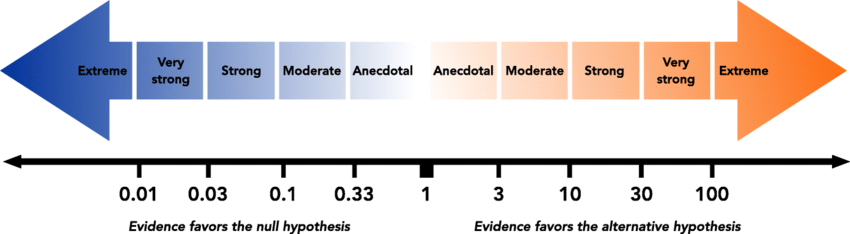
\includegraphics[width=\linewidth,height=2cm,keepaspectratio]{./figures/Lee-and-Wagenmakers-classification-scheme-for-interpreting-Bayes-factors.png}
\end{center}

\normalsize
\end{frame}

\begin{frame}[fragile]{Tests --- example of comparison of 2 nested
models}
\protect\phantomsection\label{tests-example-of-comparison-of-2-nested-models-3}
\textcolor{red}{Is our model better than intercept-only model (i.e. null model)?}

Posterior inclusion probability comparing 2 LM using \{nimble\}

\scriptsize

\begin{Shaded}
\begin{Highlighting}[]
\NormalTok{code\_pip }\OtherTok{\textless{}{-}} \FunctionTok{nimbleCode}\NormalTok{(\{}
\NormalTok{  incl }\SpecialCharTok{\textasciitilde{}} \FunctionTok{dbin}\NormalTok{(p\_incl, }\DecValTok{1}\NormalTok{) }\CommentTok{\# we add a switch}
  \ControlFlowTok{for}\NormalTok{ (i }\ControlFlowTok{in} \FunctionTok{seq\_len}\NormalTok{(N)) \{}
\NormalTok{    size[i] }\SpecialCharTok{\textasciitilde{}} \FunctionTok{dnorm}\NormalTok{(}
  \AttributeTok{mean =}\NormalTok{ intercept }\SpecialCharTok{+}\NormalTok{ incl}\SpecialCharTok{*}\NormalTok{slope}\SpecialCharTok{*}\NormalTok{humans\_eaten[i], }\AttributeTok{sd =}\NormalTok{ sigma)}
\NormalTok{  \}}
  \CommentTok{\# priors}
\NormalTok{  intercept }\SpecialCharTok{\textasciitilde{}} \FunctionTok{dnorm}\NormalTok{(}\AttributeTok{mean =} \DecValTok{50}\NormalTok{, }\AttributeTok{sd =} \DecValTok{5}\NormalTok{)}
\NormalTok{  slope }\SpecialCharTok{\textasciitilde{}} \FunctionTok{dnorm}\NormalTok{(}\AttributeTok{mean =} \DecValTok{0}\NormalTok{, }\AttributeTok{sd =} \DecValTok{5}\NormalTok{)}
\NormalTok{  sigma }\SpecialCharTok{\textasciitilde{}} \FunctionTok{dunif}\NormalTok{(}\AttributeTok{min =} \DecValTok{0}\NormalTok{, }\AttributeTok{max =} \DecValTok{5}\NormalTok{)}
\NormalTok{\})}

\NormalTok{constants\_pip }\OtherTok{\textless{}{-}} \FunctionTok{list}\NormalTok{(}\AttributeTok{p\_incl =} \FloatTok{0.5}\NormalTok{, }\AttributeTok{N =} \FunctionTok{nrow}\NormalTok{(Alien), }\AttributeTok{humans\_eaten =}\NormalTok{ Alien}\SpecialCharTok{$}\NormalTok{humans\_eaten)}

\NormalTok{inits\_pip }\OtherTok{\textless{}{-}} \FunctionTok{list}\NormalTok{(}\AttributeTok{intercept =} \FunctionTok{mean}\NormalTok{(Alien}\SpecialCharTok{$}\NormalTok{size), }\AttributeTok{slope =} \DecValTok{0}\NormalTok{, }\AttributeTok{sigma =} \DecValTok{1}\NormalTok{)}
\end{Highlighting}
\end{Shaded}

\normalsize

\footnotesize

\textbf{NB:}

\begin{itemize}
\tightlist
\item
  \texttt{p\_incl} is fixed at 0.5, which reflects a neutral prior
  belief
\item
  if several predictors were present, \texttt{incl} would have to be
  multiplied to all corresponding regression coefficients
\end{itemize}
\end{frame}

\begin{frame}[fragile]{Tests --- example of comparison of 2 nested
models}
\protect\phantomsection\label{tests-example-of-comparison-of-2-nested-models-4}
\textcolor{red}{Is our model better than intercept-only model (i.e. null model)?}

Posterior inclusion probability comparing 2 LM using \{nimble\}

\scriptsize

\begin{Shaded}
\begin{Highlighting}[]
\NormalTok{fit\_alien\_lm\_nimb\_pip }\OtherTok{\textless{}{-}} \FunctionTok{nimbleMCMC}\NormalTok{(}\AttributeTok{code =}\NormalTok{ code\_pip,}
                                    \AttributeTok{constants =}\NormalTok{ constants\_pip,}
                                    \AttributeTok{data =} \FunctionTok{list}\NormalTok{(}\AttributeTok{size =}\NormalTok{ Alien}\SpecialCharTok{$}\NormalTok{size),}
                                    \AttributeTok{inits =}\NormalTok{ inits\_pip,}
                                    \AttributeTok{nchains =} \DecValTok{4}\NormalTok{, }\AttributeTok{setSeed =} \DecValTok{1}\SpecialCharTok{:}\DecValTok{4}\NormalTok{,}
                                    \AttributeTok{nburnin =} \DecValTok{4000}\NormalTok{,}
                                    \AttributeTok{progressBar =} \ConstantTok{FALSE}\NormalTok{)}

\NormalTok{proba\_incl }\OtherTok{\textless{}{-}} \FunctionTok{mean}\NormalTok{(}\FunctionTok{sapply}\NormalTok{(fit\_alien\_lm\_nimb\_pip, \textbackslash{}(chain) }\FunctionTok{mean}\NormalTok{(chain[, }\StringTok{"incl"}\NormalTok{]))) }\CommentTok{\# avg across chains}
\NormalTok{proba\_incl}
\end{Highlighting}
\end{Shaded}

\begin{verbatim}
[1] 0.950375
\end{verbatim}

\normalsize

\pause

\bluebold{Interpretation}

\scriptsize

\begin{enumerate}
\tightlist
\item
  there is a 95\% posterior probability that the effect of the number of
  humans eaten on the size of aliens is present, versus a 5\% posterior
  probability that the data are equally consistent with the null model
\item
  since \texttt{p\_incl} is fixed at 0.5, \texttt{proba\_incl} directly
  determines BF which reduces to
  \(\dfrac{\text{proba\_incl}}{(1-\text{proba\_incl})}=\) 19.2 (note,
  this is a bit different from \{brms\} BF because the latter internally
  centres the regressors which are multiplied to priors draws)
\end{enumerate}
\end{frame}

\begin{frame}[fragile]{Tests --- example of test on parameters}
\protect\phantomsection\label{tests-example-of-test-on-parameters}
\textcolor{red}{Are parameter estimates likely to be null?}

t-tests testing \(H_0\) that the parameter estimates are 0

\footnotesize

\begin{Shaded}
\begin{Highlighting}[]
\FunctionTok{summary}\NormalTok{(fit\_alien\_lm)}\SpecialCharTok{$}\NormalTok{coefficients }\CommentTok{\# or just summary(fit\_alien\_lm)}
\end{Highlighting}
\end{Shaded}

\begin{verbatim}
              Estimate Std. Error   t value     Pr(>|t|)
(Intercept)  48.835310  1.3454140 36.297608 5.987821e-12
humans_eaten  2.374922  0.6228057  3.813263 3.410945e-03
\end{verbatim}

\normalsize

\bluebold{Interpretation:} both parameters are significantly different
from 0

\textbf{NB:}

\begin{itemize}
\tightlist
\item
  this is directly provided by the summary tables seen earlier
\end{itemize}
\end{frame}

\begin{frame}[fragile]{Tests --- example of test on parameters}
\protect\phantomsection\label{tests-example-of-test-on-parameters-1}
\textcolor{red}{Are parameter estimates likely to be null?}

using credibility intervals for testing \(H_0\) that the parameter
estimates are 0

\footnotesize

\begin{Shaded}
\begin{Highlighting}[]
\FunctionTok{fixef}\NormalTok{(fit\_alien\_lm\_brms) }\CommentTok{\# or just summary(fit\_alien\_lm\_brms)}
\end{Highlighting}
\end{Shaded}

\begin{verbatim}
             Estimate Est.Error       Q2.5     Q97.5
Intercept    48.82913 1.5129858 45.8069388 51.849559
humans_eaten  2.37829 0.6995441  0.9932649  3.758505
\end{verbatim}

\normalsize

\bluebold{Interpretation:} 0 is not among the values considered
plausible at the 95\% credible level

\textbf{NB:}

\begin{itemize}
\tightlist
\item
  this is again provided by the summary tables seen earlier
\end{itemize}
\end{frame}

\begin{frame}{Tests --- conclusions}
\protect\phantomsection\label{tests-conclusions}
\begin{itemize}
\tightlist
\item
  testing parameters directly is much easier but it increases the risk
  of false positives when null hypothesis significance testing (NHST) is
  applied (this is why I recommended earlier the testing order going
  from overall to specific)
\end{itemize}

\vspace{1em}

\begin{itemize}
\tightlist
\item
  in Bayesian statistics, the ordering isn't needed for formal
  error-rate control (unlike NHST), but the same order remains good
  scientific practice: conclusions about a coefficient are only
  meaningful if the broader model/variable is itself supported by the
  data
\end{itemize}

\vspace{1em}

\begin{itemize}
\tightlist
\item
  in Bayesian statistics, the Bayes factor is appealing as it can
  potentially be applied to all testing situations, however it is very
  dependent on priors and thus on internal scaling of variables by
  software, which makes it a measure difficult to compare across
  studies, casting doubt on the usual ``scale'' of strength of evidence
  it is associated with
\end{itemize}

\vspace{1em}

\begin{itemize}
\tightlist
\item
  in Bayesian statistics, under any continuous prior, a genuinely
  continuous slope is never exactly zero \(\rightarrow\) \(H_0\) has no
  special status but is considered as just one hypothesis among many
\end{itemize}
\end{frame}

\section{Model construction}\label{model-construction}

\begin{frame}[c]{Model construction --- core principles}
\protect\phantomsection\label{model-construction-core-principles}
\begin{itemize}
\item
  take time to imagine/research the data generating process
\item
  build your model using your knowledge \& not by trials and errors
\item
  straight lines are not your only options\\
  (e.g.~polynomial, discretisation, general additive models)
\item
  keep in mind that your ambition should be kept in check by the amount
  of data you have
\end{itemize}

\(\rightarrow\) rule of thumb: you should not estimate more than
\textasciitilde{} N/10 parameters\\
(if you want to estimate more parameters than that, collect more data)
\end{frame}

\begin{frame}{Model construction --- model simplification}
\protect\phantomsection\label{model-construction-model-simplification}
There are pros and cons of adding an additional parameter to a model:

Pros:

\begin{itemize}
\tightlist
\item
  it increases power (if it explains something)
\item
  it increases understanding
\end{itemize}

\pause

Cons:

\begin{itemize}
\tightlist
\item
  it reduces power (if it explains nothing)
\item
  it can lead to
  \blueit{overfitting}\footnote{describing patterns that are only true in the sample on hand but not in the population}
\item
  it impedes the reliability of the estimation of other parameters
  (e.g.~due to \blueit{multicollinearity})
\end{itemize}

\pause

\(\rightarrow\) this simple observation suggests a very controversial
practice in Ecology: \blueit{model simplification}, i.e.~the activity of
starting from a full model (the one with all the covariates of
interest), and then proceeding to reduce the number of variables (and
thus of parameters) by discarding the ``unimportant'' ones
\end{frame}

\begin{frame}{Model construction --- model simplification}
\protect\phantomsection\label{model-construction-model-simplification-1}
Is model simplification OK?

\pause

\bluebold{No!}

\begin{itemize}
\tightlist
\item
  it increases the rate of false positives tremendously
\item
  it increases the risk of overfitting the data
\item
  the tests, credible intervals and confidence intervals fail to capture
  and propagate the uncertainty of the model selection procedure itself
\item
  the noise alone can influence which variable is kept and which is not
\end{itemize}

\(\rightarrow\) just don't do it!
\end{frame}

\begin{frame}{Model construction --- model simplification}
\protect\phantomsection\label{model-construction-model-simplification-2}
Is model simplification OK?

\bluebold{No!}

Instead,

\begin{itemize}
\tightlist
\item
  \bluenorm{simple recommendation:} stick to a single
  \blueit{full model} that is not too complex
\item
  \bluenorm{acceptable leeway:} drop very weak interactions\\
  (the statistical drawbacks are compensated by the large gain in the
  simplicity of interpretations)
\item
  \bluenorm{alternatives:} perform \blueit{model averaging} (a weighted
  combination of estimates across alternative models) or rely on
  techniques of
  \blueit{penalisation}\footnote{a single model with many parameters is used but \blueit{shrinkage} is applied on estimates (frequentist) or on prior distributions (Bayesian) to prevent overfit}
\end{itemize}
\end{frame}

\section{Assumptions}\label{assumptions}

\begin{frame}[fragile]{Assumptions --- LM}
\protect\phantomsection\label{assumptions-lm}
\small

\bluebold{Linearity}

\begin{itemize}
\tightlist
\item
  if not, transformation of the dependent or independent variables,
  inclusion of other independent variables, interactions, or the use of
  non-linear models (e.g.~additive models) can help
\end{itemize}

\pause

\bluebold{Predictor variables are error-free}

\begin{itemize}
\tightlist
\item
  if not, adding latent variables is straightforward with a Bayesian
  approach
\end{itemize}

\pause

\bluebold{Errors are independently, identically, and normally distributed}

\begin{itemize}
\item
  there are many reasons that could cause a departure from these
  assumptions, and the appropriate remedy depends on the cause:

  \begin{itemize}
  \tightlist
  \item
    outliers \(\rightarrow\) \blueit{robust regressions}
    (e.g.~\texttt{MASS::rlm()})
  \item
    heteroscedasticity caused by predictor \(\rightarrow\)
    \blueit{heteroscedastic} LM (e.g.~\texttt{spaMM::fitme()} with
    \texttt{resid.model})
  \item
    heteroscedasticity caused by a mean-variance relationship
    \(\rightarrow\) GLM
  \item
    dependence caused by spatial or temporal proximity \(\rightarrow\)
    \blueit{autoregressive model} (e.g.~\texttt{AR1()},
    \texttt{Matern()} in \{spaMM\})
  \item
    dependence caused by shared origin \(\rightarrow\)
    \blueit{linear mixed-effect models} (LMM)
  \end{itemize}
\end{itemize}
\end{frame}

\begin{frame}[fragile]{Assumptions --- LM}
\protect\phantomsection\label{assumptions-lm-1}
You can test all the assumptions about the errors by eye:

\footnotesize

\begin{Shaded}
\begin{Highlighting}[]
\FunctionTok{par}\NormalTok{(}\AttributeTok{mfrow =} \FunctionTok{c}\NormalTok{(}\DecValTok{2}\NormalTok{, }\DecValTok{3}\NormalTok{))}
\FunctionTok{plot}\NormalTok{(fit\_flipper\_3var, }\AttributeTok{which =} \DecValTok{1}\SpecialCharTok{:}\DecValTok{6}\NormalTok{)}
\end{Highlighting}
\end{Shaded}

\begin{center}
\includegraphics[width=\linewidth,height=6cm,keepaspectratio]{modelling_intro_files/figure-beamer/unnamed-chunk-35-1.pdf}
\end{center}

\normalsize
\end{frame}

\begin{frame}[fragile]{Assumptions --- LM}
\protect\phantomsection\label{assumptions-lm-2}
You can check the
leverage\footnote{how unusual one row of the design matrix is} and
influence\footnote{how strongly an observation impacts the predicted value}
of each point easily:

\footnotesize

\begin{Shaded}
\begin{Highlighting}[]
\FunctionTok{as\_tibble}\NormalTok{(}\FunctionTok{influence.measures}\NormalTok{(fit\_flipper\_3var)}\SpecialCharTok{$}\NormalTok{infmat)}
\end{Highlighting}
\end{Shaded}

\begin{verbatim}
# A tibble: 333 x 9
    dfb.1_ dfb.flp_ dfb.sxml  dfb.spcC dfb.spcG   dffit cov.r    cook.d     hat
     <dbl>    <dbl>    <dbl>     <dbl>    <dbl>   <dbl> <dbl>     <dbl>   <dbl>
1 -0.0166   0.0163   -0.0148  0.000177 -0.0115  -0.0211 1.04  0.0000896 0.0244 
2  0.0181  -0.00986  -0.0659 -0.0625   -0.0266   0.150  0.991 0.00450   0.00990
3  0.0741  -0.0797    0.0877  0.0714    0.0953  -0.127  1.02  0.00322   0.0163 
4  0.00928 -0.0102    0.0131  0.0109    0.0132  -0.0195 1.03  0.0000766 0.0136 
5 -0.0394   0.0371   -0.0704  0.0347   -0.00728 -0.115  1.01  0.00263   0.0110 
# i 328 more rows
\end{verbatim}

\normalsize
\end{frame}

\begin{frame}[fragile]{Assumptions --- GLM}
\protect\phantomsection\label{assumptions-glm}
\bluebold{Model structure}

\begin{itemize}
\tightlist
\item
  linearity (for the linear predictor)
\item
  lack of perfect multicollinearity
\item
  predictor variables have fixed values
\end{itemize}

\bluebold{Errors}

\begin{itemize}
\tightlist
\item
  independence (no serial autocorrelation)
\item
  lack of \blueit{overdispersion} and \blueit{underdispersion} (see next
  slide)
\end{itemize}

\texttt{plot(fit)} is not helpful in this case since expectations are
not like those of a LM; instead, the package \{DHARMa\} can help you
test some of these assumptions (eventhough the approach it uses is not
flawless)
\end{frame}

\begin{frame}[fragile]{Assumptions --- GLM}
\protect\phantomsection\label{assumptions-glm-1}
A GLM assumes a particular relationship between mu and var(mu):

\footnotesize

\begin{Shaded}
\begin{Highlighting}[]
\NormalTok{p }\OtherTok{\textless{}{-}} \FunctionTok{seq}\NormalTok{(}\DecValTok{0}\NormalTok{, }\DecValTok{1}\NormalTok{, }\FloatTok{0.1}\NormalTok{); lambda }\OtherTok{\textless{}{-}} \DecValTok{0}\SpecialCharTok{:}\DecValTok{10}\NormalTok{; theta }\OtherTok{\textless{}{-}} \DecValTok{0}\SpecialCharTok{:}\DecValTok{10}
\NormalTok{v\_b }\OtherTok{\textless{}{-}} \FunctionTok{binomial}\NormalTok{()}\SpecialCharTok{$}\FunctionTok{variance}\NormalTok{(p)}
\NormalTok{v\_p }\OtherTok{\textless{}{-}} \FunctionTok{poisson}\NormalTok{()}\SpecialCharTok{$}\FunctionTok{variance}\NormalTok{(lambda)}
\NormalTok{v\_G }\OtherTok{\textless{}{-}} \FunctionTok{Gamma}\NormalTok{()}\SpecialCharTok{$}\FunctionTok{variance}\NormalTok{(theta)}
\FunctionTok{par}\NormalTok{(}\AttributeTok{mfrow =} \FunctionTok{c}\NormalTok{(}\DecValTok{1}\NormalTok{, }\DecValTok{3}\NormalTok{), }\AttributeTok{las =} \DecValTok{1}\NormalTok{, }\AttributeTok{cex =} \FloatTok{1.5}\NormalTok{)}
\FunctionTok{plot}\NormalTok{(v\_b }\SpecialCharTok{\textasciitilde{}}\NormalTok{ p, }\AttributeTok{type =} \StringTok{"o"}\NormalTok{)}
\FunctionTok{plot}\NormalTok{(v\_p }\SpecialCharTok{\textasciitilde{}}\NormalTok{ lambda, }\AttributeTok{type =} \StringTok{"o"}\NormalTok{)}
\FunctionTok{plot}\NormalTok{(v\_G }\SpecialCharTok{\textasciitilde{}}\NormalTok{ theta, }\AttributeTok{type =} \StringTok{"o"}\NormalTok{)}
\end{Highlighting}
\end{Shaded}

\begin{center}
\includegraphics[width=\linewidth,height=4cm,keepaspectratio]{modelling_intro_files/figure-beamer/unnamed-chunk-37-1.pdf}
\end{center}

\normalsize
\end{frame}

\begin{frame}{Assumptions --- GLM}
\protect\phantomsection\label{assumptions-glm-2}
A GLM assumes a particular relationship between mu and var(mu)

\begin{itemize}
\item
  if the variance increases faster than assumed, there is
  \blueit{overdispersion} (frequent)
\item
  if the variance increases more slowly than assumed, there is
  \blueit{underdispersion} (rare)
\end{itemize}

\pause

\vspace{1em}

Typical situation: count data are overdispersed compared to Poisson
expectation

\(\rightarrow\) \blueit{negative binomial model} (e.g.~\{spaMM\},
\{glmmTMB\}, \{brms\}, \{nimble\}) and/or \blueit{zero-augmented models}
(e.g.~\{glmmTMB\}, \{brms\}, \{nimble\})
\end{frame}

\section{Habitat occupancy model}\label{habitat-occupancy-model}

\begin{frame}{Habitat occupancy model --- recall the situation}
\protect\phantomsection\label{habitat-occupancy-model-recall-the-situation}
\begin{center}
\resizebox{0.5\linewidth}{!}{%
\begin{forest}
for tree={
  align=center,
  parent anchor=south,
  child anchor=north,
  edge={-latex, thick},
  l sep=10mm,
  s sep=2mm,
  font=\small,
}
[{population}
  [{presence}, edge label={node[midway, anchor=east, xshift=-10pt, font=\small]{$P(\mathrm{occupancy}) = \psi$}}
    [{detected\\(true positive)}, draw, rounded corners, fill=gray!10,
      edge label={node[midway, anchor=east, yshift=-5pt, xshift=-10pt, font=\scriptsize, align=center]{$P(\mathrm{detection}) = p_{11}$}}]
    [{not detected\\ (false negative)}, draw, rounded corners, fill=gray!10,
      edge label={node[midway, anchor=west, yshift=-5pt, xshift=10pt,  font=\scriptsize, align=center]{$1 - p_{11}$}}]
  ]
  [{absence}, edge label={node[midway, anchor=west, xshift=10pt, font=\small]{$1 - \psi$}}
    [{not detected\\ (true negative)}, draw, rounded corners, fill=gray!10,
      edge label={node[midway, anchor=west, font=\scriptsize]{$1$}}]
  ]
]
\end{forest}
}
\end{center}

We thus have a state space model (SSM):

\begin{itemize}
\tightlist
\item
  a non-observable layer with a state variable describing whether the
  habitat is occupied or not
\item
  an observable outcome describing whether a particular species has been
  observed or not
\item
  each of these levels can be modelled by a logistic GLM
\item
  the 2 GLMs are not independent, it is a hierarchical model
\end{itemize}
\end{frame}

\begin{frame}[fragile]{Habitat occupancy model --- fitting a no
covariate model}
\protect\phantomsection\label{habitat-occupancy-model-fitting-a-no-covariate-model}
We first simulate data and define the model

\scriptsize

\begin{Shaded}
\begin{Highlighting}[]
\NormalTok{n\_sites }\OtherTok{\textless{}{-}} \DecValTok{100}
\NormalTok{n\_visits }\OtherTok{\textless{}{-}} \DecValTok{50}

\FunctionTok{set.seed}\NormalTok{(}\DecValTok{123}\NormalTok{)}
\NormalTok{prob\_occu }\OtherTok{\textless{}{-}} \FloatTok{0.3}\NormalTok{; cond\_prob\_obs }\OtherTok{\textless{}{-}} \FloatTok{0.1}  \CommentTok{\# simulated truth}

\NormalTok{occu\_truth }\OtherTok{\textless{}{-}} \FunctionTok{rbinom}\NormalTok{(}\AttributeTok{n =}\NormalTok{ n\_sites, }\AttributeTok{size =} \DecValTok{1}\NormalTok{, }\AttributeTok{prob =}\NormalTok{ prob\_occu)}

\NormalTok{obs\_mat }\OtherTok{\textless{}{-}} \FunctionTok{matrix}\NormalTok{(}\ConstantTok{NA}\NormalTok{, }\AttributeTok{nrow =}\NormalTok{ n\_sites, }\AttributeTok{ncol =}\NormalTok{ n\_visits)}

\ControlFlowTok{for}\NormalTok{ (site }\ControlFlowTok{in} \FunctionTok{seq\_len}\NormalTok{(n\_sites)) \{}
\NormalTok{  obs\_mat[site, ] }\OtherTok{\textless{}{-}}\NormalTok{ occu\_truth[site] }\SpecialCharTok{*} \FunctionTok{rbinom}\NormalTok{(n\_visits, }\AttributeTok{size =} \DecValTok{1}\NormalTok{, }\AttributeTok{prob =}\NormalTok{ cond\_prob\_obs)}
\NormalTok{\}}

\NormalTok{code\_occu }\OtherTok{\textless{}{-}} \FunctionTok{nimbleCode}\NormalTok{(\{}
  \ControlFlowTok{for}\NormalTok{ (site }\ControlFlowTok{in} \FunctionTok{seq\_len}\NormalTok{(n\_sites)) \{}
\NormalTok{    z[site] }\SpecialCharTok{\textasciitilde{}} \FunctionTok{dbern}\NormalTok{(}\AttributeTok{prob =}\NormalTok{ psi) }\CommentTok{\# occupancy status}
\NormalTok{    p[site] }\OtherTok{\textless{}{-}}\NormalTok{ z[site] }\SpecialCharTok{*}\NormalTok{ p\_cond  }\CommentTok{\# detection prob}
    \ControlFlowTok{for}\NormalTok{ (visit }\ControlFlowTok{in} \FunctionTok{seq\_len}\NormalTok{(n\_visits)) \{}
\NormalTok{      y[site, visit] }\SpecialCharTok{\textasciitilde{}} \FunctionTok{dbern}\NormalTok{(p[site]) }\CommentTok{\# observation outcome}
\NormalTok{    \}}
\NormalTok{  \}}
\NormalTok{  psi }\SpecialCharTok{\textasciitilde{}} \FunctionTok{dunif}\NormalTok{(}\DecValTok{0}\NormalTok{, }\DecValTok{1}\NormalTok{); p\_cond }\SpecialCharTok{\textasciitilde{}} \FunctionTok{dunif}\NormalTok{(}\DecValTok{0}\NormalTok{, }\DecValTok{1}\NormalTok{)}
\NormalTok{\})}
\end{Highlighting}
\end{Shaded}

\normalsize
\end{frame}

\begin{frame}[fragile]{Habitat occupancy model --- fitting a no
covariate model}
\protect\phantomsection\label{habitat-occupancy-model-fitting-a-no-covariate-model-1}
We can now fit the model

\scriptsize

\begin{Shaded}
\begin{Highlighting}[]
\NormalTok{constants\_occu }\OtherTok{\textless{}{-}} \FunctionTok{list}\NormalTok{(}\AttributeTok{n\_sites =}\NormalTok{ n\_sites, }\AttributeTok{n\_visits =}\NormalTok{ n\_visits)}

\NormalTok{z\_init }\OtherTok{\textless{}{-}} \FunctionTok{as.numeric}\NormalTok{(}\FunctionTok{rowSums}\NormalTok{(obs\_mat) }\SpecialCharTok{\textgreater{}} \DecValTok{0}\NormalTok{) }\CommentTok{\# initialise z: any detection {-}\textgreater{} known occupied}
\NormalTok{inits\_occu }\OtherTok{\textless{}{-}} \FunctionTok{list}\NormalTok{(}\AttributeTok{p\_cond =} \FloatTok{0.5}\NormalTok{, }\AttributeTok{psi =} \FloatTok{0.1}\NormalTok{, }\AttributeTok{z =}\NormalTok{ z\_init)}

\NormalTok{fit\_occu }\OtherTok{\textless{}{-}} \FunctionTok{nimbleMCMC}\NormalTok{(}\AttributeTok{code =}\NormalTok{ code\_occu,}
                       \AttributeTok{constants =}\NormalTok{ constants\_occu,}
                       \AttributeTok{data =} \FunctionTok{list}\NormalTok{(}\AttributeTok{y =}\NormalTok{ obs\_mat),}
                       \AttributeTok{inits =}\NormalTok{ inits\_occu,}
                       \AttributeTok{nchains =} \DecValTok{4}\NormalTok{, }\AttributeTok{setSeed =} \DecValTok{1}\SpecialCharTok{:}\DecValTok{4}\NormalTok{,}
                       \AttributeTok{niter =} \DecValTok{10000}\NormalTok{, }\AttributeTok{nburnin =} \DecValTok{4000}\NormalTok{,}
                       \AttributeTok{progressBar =} \ConstantTok{FALSE}\NormalTok{)}

\FunctionTok{summary}\NormalTok{(}\FunctionTok{as\_draws}\NormalTok{(fit\_occu))}
\end{Highlighting}
\end{Shaded}

\begin{verbatim}
# A tibble: 2 x 10
  variable   mean median      sd     mad     q5    q95  rhat ess_bulk ess_tail
  <chr>     <dbl>  <dbl>   <dbl>   <dbl>  <dbl>  <dbl> <dbl>    <dbl>    <dbl>
1 p_cond   0.0821 0.0820 0.00728 0.00728 0.0704 0.0942  1.00    5465.    5864.
2 psi      0.299  0.298  0.0459  0.0474  0.227  0.377   1.00    5211.    5583.
\end{verbatim}

\normalsize
\end{frame}

\begin{frame}[fragile]{Habitat occupancy model --- fitting a model with
covariates}
\protect\phantomsection\label{habitat-occupancy-model-fitting-a-model-with-covariates}
We first simulate data

\scriptsize

\begin{Shaded}
\begin{Highlighting}[]
\NormalTok{n\_sites }\OtherTok{\textless{}{-}} \DecValTok{100}
\NormalTok{n\_visits }\OtherTok{\textless{}{-}} \DecValTok{50}

\FunctionTok{set.seed}\NormalTok{(}\DecValTok{123}\NormalTok{)}
\NormalTok{prob\_occu }\OtherTok{\textless{}{-}} \FloatTok{0.3}  \CommentTok{\# simulated truth}
\NormalTok{occu\_truth }\OtherTok{\textless{}{-}} \FunctionTok{rbinom}\NormalTok{(}\AttributeTok{n =}\NormalTok{ n\_sites, }\AttributeTok{size =} \DecValTok{1}\NormalTok{, }\AttributeTok{prob =}\NormalTok{ prob\_occu)}

\NormalTok{covar\_detect\_site }\OtherTok{\textless{}{-}} \FunctionTok{rnorm}\NormalTok{(}\AttributeTok{n =}\NormalTok{ n\_sites) }\CommentTok{\# site{-}level covariate}

\CommentTok{\# visit{-}level covariate, varies per site AND visit}
\NormalTok{covar\_detect\_visit }\OtherTok{\textless{}{-}} \FunctionTok{matrix}\NormalTok{(}\FunctionTok{rnorm}\NormalTok{(}\AttributeTok{n =}\NormalTok{ n\_sites }\SpecialCharTok{*}\NormalTok{ n\_visits), }\AttributeTok{nrow =}\NormalTok{ n\_sites, }\AttributeTok{ncol =}\NormalTok{ n\_visits)}

\CommentTok{\# simulated truth for effect of covariates}
\NormalTok{beta0\_true }\OtherTok{\textless{}{-}} \SpecialCharTok{{-}}\DecValTok{2}   \CommentTok{\# intercept}
\NormalTok{beta1\_true }\OtherTok{\textless{}{-}} \DecValTok{1}    \CommentTok{\# site{-}level covariate slope}
\NormalTok{beta2\_true }\OtherTok{\textless{}{-}} \FloatTok{0.5}  \CommentTok{\# visit{-}level covariate slope}

\NormalTok{p\_true }\OtherTok{\textless{}{-}} \FunctionTok{plogis}\NormalTok{(beta0\_true }\SpecialCharTok{+}
\NormalTok{                 beta1\_true }\SpecialCharTok{*}\NormalTok{ covar\_detect\_site }\SpecialCharTok{+} \CommentTok{\# recycled across visits}
\NormalTok{                 beta2\_true }\SpecialCharTok{*}\NormalTok{ covar\_detect\_visit) }\CommentTok{\# site x visit matrix}

\NormalTok{obs\_mat }\OtherTok{\textless{}{-}} \FunctionTok{matrix}\NormalTok{(}\ConstantTok{NA\_real\_}\NormalTok{, }\AttributeTok{nrow =}\NormalTok{ n\_sites, }\AttributeTok{ncol =}\NormalTok{ n\_visits)}

\ControlFlowTok{for}\NormalTok{ (site }\ControlFlowTok{in} \FunctionTok{seq\_len}\NormalTok{(n\_sites))}
\NormalTok{  obs\_mat[site, ] }\OtherTok{\textless{}{-}}\NormalTok{ occu\_truth[site] }\SpecialCharTok{*} \FunctionTok{rbinom}\NormalTok{(n\_visits, }\AttributeTok{size =} \DecValTok{1}\NormalTok{, }\AttributeTok{prob =}\NormalTok{ p\_true[site, ])}
\end{Highlighting}
\end{Shaded}

\normalsize
\end{frame}

\begin{frame}[fragile]{Habitat occupancy model --- fitting a model with
covariates}
\protect\phantomsection\label{habitat-occupancy-model-fitting-a-model-with-covariates-1}
We then define the model

\scriptsize

\begin{Shaded}
\begin{Highlighting}[]
\NormalTok{code\_occu }\OtherTok{\textless{}{-}} \FunctionTok{nimbleCode}\NormalTok{(\{}
  \ControlFlowTok{for}\NormalTok{ (site }\ControlFlowTok{in} \FunctionTok{seq\_len}\NormalTok{(n\_sites)) \{}
    
\NormalTok{    z[site] }\SpecialCharTok{\textasciitilde{}} \FunctionTok{dbern}\NormalTok{(}\AttributeTok{prob =}\NormalTok{ psi)}
    
    \ControlFlowTok{for}\NormalTok{ (visit }\ControlFlowTok{in} \FunctionTok{seq\_len}\NormalTok{(n\_visits)) \{}
      
      \FunctionTok{logit}\NormalTok{(p\_cond[site, visit]) }\OtherTok{\textless{}{-}}\NormalTok{ beta0 }\SpecialCharTok{+}
\NormalTok{        beta1 }\SpecialCharTok{*}\NormalTok{ covar\_detect\_site[site] }\SpecialCharTok{+}
\NormalTok{        beta2 }\SpecialCharTok{*}\NormalTok{ covar\_detect\_visit[site, visit]}
      
\NormalTok{      p[site, visit] }\OtherTok{\textless{}{-}}\NormalTok{ z[site] }\SpecialCharTok{*}\NormalTok{ p\_cond[site, visit]}
      
\NormalTok{      y[site, visit] }\SpecialCharTok{\textasciitilde{}} \FunctionTok{dbern}\NormalTok{(p[site, visit])}
\NormalTok{    \}}
\NormalTok{  \}}
  
\NormalTok{  psi }\SpecialCharTok{\textasciitilde{}} \FunctionTok{dunif}\NormalTok{(}\DecValTok{0}\NormalTok{, }\DecValTok{1}\NormalTok{)}
\NormalTok{  beta0 }\SpecialCharTok{\textasciitilde{}} \FunctionTok{dnorm}\NormalTok{(}\DecValTok{0}\NormalTok{, }\AttributeTok{sd =} \DecValTok{10}\NormalTok{)}
\NormalTok{  beta1 }\SpecialCharTok{\textasciitilde{}} \FunctionTok{dnorm}\NormalTok{(}\DecValTok{0}\NormalTok{, }\AttributeTok{sd =} \DecValTok{10}\NormalTok{)}
\NormalTok{  beta2 }\SpecialCharTok{\textasciitilde{}} \FunctionTok{dnorm}\NormalTok{(}\DecValTok{0}\NormalTok{, }\AttributeTok{sd =} \DecValTok{10}\NormalTok{)}
\NormalTok{\})}
\end{Highlighting}
\end{Shaded}

\normalsize
\end{frame}

\begin{frame}[fragile]{Habitat occupancy model --- fitting a model with
covariates}
\protect\phantomsection\label{habitat-occupancy-model-fitting-a-model-with-covariates-2}
We then set the constant and initialise the model

\footnotesize

\begin{Shaded}
\begin{Highlighting}[]
\NormalTok{constants\_occu }\OtherTok{\textless{}{-}} \FunctionTok{list}\NormalTok{(}\AttributeTok{n\_sites =}\NormalTok{ n\_sites,}
                       \AttributeTok{n\_visits =}\NormalTok{ n\_visits,}
                       \AttributeTok{covar\_detect\_site =}\NormalTok{ covar\_detect\_site,}
                       \AttributeTok{covar\_detect\_visit =}\NormalTok{ covar\_detect\_visit)}

\NormalTok{z\_init }\OtherTok{\textless{}{-}} \FunctionTok{as.numeric}\NormalTok{(}\FunctionTok{rowSums}\NormalTok{(obs\_mat) }\SpecialCharTok{\textgreater{}} \DecValTok{0}\NormalTok{) }\CommentTok{\# initialise z: any detection {-}\textgreater{} known occupied}

\NormalTok{inits\_occu }\OtherTok{\textless{}{-}} \ControlFlowTok{function}\NormalTok{() \{}
  \FunctionTok{list}\NormalTok{(}\AttributeTok{psi =} \FunctionTok{runif}\NormalTok{(}\DecValTok{1}\NormalTok{, }\FloatTok{0.1}\NormalTok{, }\FloatTok{0.9}\NormalTok{),}
       \AttributeTok{beta0 =} \FunctionTok{rnorm}\NormalTok{(}\DecValTok{1}\NormalTok{, }\DecValTok{0}\NormalTok{, }\DecValTok{1}\NormalTok{),}
       \AttributeTok{beta1 =} \FunctionTok{rnorm}\NormalTok{(}\DecValTok{1}\NormalTok{, }\DecValTok{0}\NormalTok{, }\DecValTok{1}\NormalTok{),}
       \AttributeTok{beta2 =} \FunctionTok{rnorm}\NormalTok{(}\DecValTok{1}\NormalTok{, }\DecValTok{0}\NormalTok{, }\DecValTok{1}\NormalTok{),}
       \AttributeTok{z =}\NormalTok{ z\_init)}
\NormalTok{\}}
\end{Highlighting}
\end{Shaded}

\normalsize
\end{frame}

\begin{frame}[fragile]{Habitat occupancy model --- fitting a model with
covariates}
\protect\phantomsection\label{habitat-occupancy-model-fitting-a-model-with-covariates-3}
Finally, we fit the model

\scriptsize

\begin{Shaded}
\begin{Highlighting}[]
\NormalTok{fit\_occu }\OtherTok{\textless{}{-}} \FunctionTok{nimbleMCMC}\NormalTok{(}\AttributeTok{code =}\NormalTok{ code\_occu,}
                       \AttributeTok{constants =}\NormalTok{ constants\_occu,}
                       \AttributeTok{data =} \FunctionTok{list}\NormalTok{(}\AttributeTok{y =}\NormalTok{ obs\_mat),}
                       \AttributeTok{inits =}\NormalTok{ inits\_occu,}
                       \AttributeTok{nchains =} \DecValTok{4}\NormalTok{, }\AttributeTok{setSeed =} \DecValTok{1}\SpecialCharTok{:}\DecValTok{4}\NormalTok{,}
                       \AttributeTok{niter =} \DecValTok{10000}\NormalTok{, }\AttributeTok{nburnin =} \DecValTok{4000}\NormalTok{,}
                       \AttributeTok{progressBar =} \ConstantTok{FALSE}\NormalTok{)}

\FunctionTok{summary}\NormalTok{(}\FunctionTok{as\_draws}\NormalTok{(fit\_occu))}
\end{Highlighting}
\end{Shaded}

\begin{verbatim}
# A tibble: 4 x 10
  variable   mean median     sd    mad     q5    q95  rhat ess_bulk ess_tail
  <chr>     <dbl>  <dbl>  <dbl>  <dbl>  <dbl>  <dbl> <dbl>    <dbl>    <dbl>
1 beta0    -2.15  -2.15  0.102  0.101  -2.32  -1.98   1.00    2309.    3468.
2 beta1     1.04   1.04  0.0951 0.0956  0.886  1.20   1.00    2552.    4260.
3 beta2     0.586  0.584 0.0833 0.0831  0.451  0.724  1.00    3917.    5680.
4 psi       0.299  0.299 0.0460 0.0458  0.224  0.376  1.00    5068.    6133.
\end{verbatim}

\normalsize

\textbf{NB:} the agreement between the true parameters and their
estimates is very good!
\end{frame}

\begin{frame}{Habitat occupancy model --- towards more realistic models}
\protect\phantomsection\label{habitat-occupancy-model-towards-more-realistic-models}
Even our complex model made some particularly crude assumptions:

\begin{itemize}
\tightlist
\item
  we considered that the true probability of occupancy was fixed
  (\(\psi=0.3\) in our example) and thus did not vary in time or space
\item
  we only look at one species in isolation
\end{itemize}

Relaxing these assumptions makes models much more complicated, but
fortunately, packages such as \{nimbleEcology\} or \{unmarked\} (a
non-Bayesian alternative) have pre-built models to help you relax these
assumptions with very little coding

Rahel will show you how to do that!
\end{frame}

\section{Conclusions}\label{conclusions}

\begin{frame}[c]{Conclusions}
\protect\phantomsection\label{conclusions-1}
\begin{itemize}
\item
  modelling can be tricky, especially when relying on MCMC
\item
  comparing the results from alternative packages relying on a different
  set of assumptions can be useful to identify issues (default settings
  are not always best)
\item
  simulating data is critical to make sure you do estimate what you
  think
\item
  \{nimble\} is very flexible and can do much more than I showed you
\end{itemize}
\end{frame}

\section*{Questions?}\label{questions}
\addcontentsline{toc}{section}{Questions?}

\begin{frame}[c]{}
\protect\phantomsection\label{section}
\centering

\Large Questions?
\end{frame}

\section*{Developer corner}\label{developer-corner}
\addcontentsline{toc}{section}{Developer corner}

\begin{frame}[c]{}
\protect\phantomsection\label{section-1}
\centering

\Large Developer corner
\end{frame}

\begin{frame}[fragile]{Ignore this slide --- (technical info for Alex)}
\protect\phantomsection\label{ignore-this-slide-technical-info-for-alex}
\tiny

\begin{verbatim}
[1] "0.3 min of R running time"
\end{verbatim}

\begin{verbatim}
R version 4.6.1 (2026-06-24)
Platform: x86_64-redhat-linux-gnu
Running under: Fedora Linux 44 (KDE Plasma Desktop Edition)

Matrix products: default
BLAS/LAPACK: FlexiBLAS OPENBLAS-OPENMP;  LAPACK version 3.12.1

attached base packages:
[1] stats     graphics  grDevices datasets  utils     methods   base     

other attached packages:
 [1] modelbased_0.16.0 bayesplot_1.15.0  posterior_1.7.0   nimble_1.4.3      brms_2.23.0       Rcpp_1.1.2        lubridate_1.9.5  
 [8] forcats_1.0.1     stringr_1.6.0     dplyr_1.2.1       purrr_1.2.2       readr_2.2.0       tidyr_1.3.2       tibble_3.3.1     
[15] ggplot2_4.0.3     tidyverse_2.0.0  

loaded via a namespace (and not attached):
 [1] Rdpack_2.6.6           gridExtra_2.3.1        inline_0.3.21          sandwich_3.1-3         rlang_1.3.0           
 [6] magrittr_2.0.5         multcomp_1.4-32        otel_0.2.0             matrixStats_1.5.0      compiler_4.6.1        
[11] loo_2.10.1             vctrs_0.7.3            reshape2_1.4.5         pkgconfig_2.0.3        crayon_1.5.3          
[16] fastmap_1.2.0          backports_1.5.1        labeling_0.4.3         utf8_1.2.6             CoprManager_0.5.8     
[21] rmarkdown_2.31         tzdb_0.5.0             pracma_2.4.6           nloptr_2.2.1           tinytex_0.60          
[26] bit_4.6.0              xfun_0.60              jsonlite_2.0.0         parallel_4.6.1         R6_2.6.1              
[31] stringi_1.8.9          RColorBrewer_1.1-3     StanHeaders_2.32.10    boot_1.3-32            numDeriv_2016.8-1.1   
[36] estimability_2.0.0     rstan_2.32.7           knitr_1.51             zoo_1.9-0              parameters_0.29.2     
[41] Matrix_1.7-6           splines_4.6.1          igraph_2.3.3           timechange_0.4.0       tidyselect_1.2.1      
[46] rstudioapi_0.19.0      abind_1.4-8            yaml_2.3.12            codetools_0.2-20       curl_7.1.0            
[51] pkgbuild_1.4.8         lattice_0.23-1         plyr_1.8.9             withr_3.0.3            bridgesampling_1.2-1  
[56] bayestestR_0.18.1      S7_0.2.2               coda_0.19-4.1          evaluate_1.0.5         marginaleffects_0.32.0
[61] survival_3.8-11        RcppParallel_6.2.0     pillar_1.11.1          tensorA_0.36.2.1       checkmate_2.3.4       
[66] stats4_4.6.1           reformulas_0.4.4       insight_1.5.2          distributional_0.8.1   generics_0.1.4        
[71] vroom_1.7.1            hms_1.1.4              rstantools_2.7.0       scales_1.4.0           minqa_1.2.8           
[76] xtable_1.8-8           glue_1.8.1             emmeans_2.0.4          tools_4.6.1            see_0.14.1            
[81] data.table_1.18.6.1    lme4_2.0-6             mvtnorm_1.4-2          grid_4.6.1             rbibutils_2.4.1       
[86] QuickJSR_1.11.0        datawizard_1.3.1       nlme_3.1-170           cli_3.6.6              Brobdingnag_1.2-9     
[91] V8_8.2.0               gtable_0.3.6           digest_0.6.39          TH.data_1.1-5          farver_2.1.2          
[96] htmltools_0.5.9        lifecycle_1.0.5        bit64_4.8.4            MASS_7.3-66           
\end{verbatim}

\normalsize
\end{frame}




\end{document}
